%%% LaTeX-Vorlage Version 1.8 %%%

% Grundlegende Dokumenteneigenschaften gemäß DHBW-Vorgaben
\documentclass[a4paper,fontsize=11pt,oneside,parskip=half,headings=normal]{scrreprt} 
% \usepackage{showframe} % nur für Kontrolle der Ränder 

%%% Präambel einbinden (mit Festlegungen gemäß DHBW-Vorgaben) %%%
%%% Präambel %%%
% hier sollten keine Änderungen erforderlich sein
%
\usepackage[utf8]{inputenc}   % Zeichencodierung UTF-8 für Eingabe-Dateien
\usepackage[T1]{fontenc}      % Darstellung von Umlauten im PDF

\usepackage{listings}         % für Einbindung von Code-Listings
\lstset{numbers=left,numberstyle=\tiny,numbersep=5pt,texcl=true}
\lstset{literate=             % erlaubt Sonderzeichen in Code-Listings 
{Ö}{{\"O}}1
{Ä}{{\"A}}1
{Ü}{{\"U}}1
{ß}{{\ss}}2
{ü}{{\"u}}1
{ä}{{\"a}}1
{ö}{{\"o}}1
{€}{{\euro}}1
}

\usepackage[
  inner=35mm,outer=15mm,top=25mm,
  bottom=20mm,foot=12mm,includefoot
]{geometry}                 % Einstellungen für Ränder

\usepackage[english]{babel} % Spracheinstellungen Englisch
\usepackage[babel,english=british]{csquotes} % englische Anf.zeichen
\usepackage{enumerate}      % anpassbare Nummerier./Aufz.
\usepackage{graphicx}       % Einbinden von Grafiken
\usepackage[onehalfspacing]{setspace} % anderthalbzeilig

\usepackage{blindtext}      % Textgenerierung für Testzwecke
\usepackage{color}          % Verwendung von Farbe 

\usepackage{acronym}        % für ein Abkürzungsverzeichnis

\usepackage[                % Biblatex
  backend=biber,
  bibstyle=_dhbw_authoryear,maxbibnames=99,
  citestyle=authoryear,     
  uniquename=true, useprefix=true,
  bibencoding=utf8]{biblatex}
%kein Punkt am Ende bei \footcite
%http://www.golatex.de/footcite-ohne-punkt-am-schluss-t4865.html
\renewcommand{\bibfootnotewrapper}[1]{\bibsentence#1}


%Reihenfolge der Autorennamen
%   
% http://golatex.de/viewtopic,p,80448.html#80448
% Argumente: siehe http://texwelt.de/blog/modifizieren-eines-biblatex-stils/
\DeclareNameFormat{sortname}{% Bibliographie
  \ifnum\value{uniquename}=0 % Normalfall
    \ifuseprefix%
      {%
         \usebibmacro{name:family-given}
           {\namepartfamily}
           {\namepartgiveni}
           {\namepartprefix}
           {\namepartsuffixi}%
       }
      {%
         \usebibmacro{name:family-given}
           {\namepartfamily}
           {\namepartgiveni}
           {\namepartprefixi}
           {\namepartsuffixi}%
       }%
  \fi
  \ifnum\value{uniquename}=1% falls nicht eindeutig, abgek. Vorname 
      {%
         \usebibmacro{name:family-given}
           {\namepartfamily}
           {\namepartgiveni}
           {\namepartprefix}
           {\namepartsuffix}%
       }%
  \fi
  \ifnum\value{uniquename}=2% falls nicht eindeutig, ganzer Vorname 
      {%
         \usebibmacro{name:family-given}
           {\namepartfamily}
           {\namepartgiven}
           {\namepartprefix}
           {\namepartsuffix}%
       }%
  \fi   
  \usebibmacro{name:andothers}}

\DeclareNameFormat{labelname}{% für Zitate
  \ifnum\value{uniquename}=0 % Normalfall
    \ifuseprefix%
      {%
         \usebibmacro{name:family-given}
           {\namepartfamily}
           {\empty}
           {\namepartprefix}
           {\namepartsuffixi}%
       }
      {%
         \usebibmacro{name:family-given}
           {\namepartfamily}
           {\empty}
           {\namepartprefixi}
           {\namepartsuffixi}%
       }%
  \fi
  \ifnum\value{uniquename}=1% falls nicht eindeutig, abgek. Vorname 
      {%
         \usebibmacro{name:family-given}
           {\namepartfamily}
           {\namepartgiveni}
           {\namepartprefix}
           {\namepartsuffix}%
       }%
  \fi
  \ifnum\value{uniquename}=2% falls nicht eindeutig, ganzer Vorname 
      {%
         \usebibmacro{name:family-given}
           {\namepartfamily}
           {\namepartgiven}
           {\namepartprefix}
           {\namepartsuffix}%
       }%
  \fi   
  \usebibmacro{name:andothers}}
      
  
\DeclareFieldFormat{extrayear}{% = the 'a' in 'Jones 1995a'
  \iffieldnums{labelyear}
    {\mknumalph{#1}}
    {\mknumalph{#1}}}        

\renewcommand*{\multinamedelim}{\addslash}
\renewcommand*{\finalnamedelim}{\addslash}
\renewcommand*{\multilistdelim}{\addslash}
\renewcommand*{\finallistdelim}{\addslash}

\renewcommand{\nameyeardelim}{~}

% Literaturverzeichnis: Doppelpunkt zwischen Name (Jahr): Rest 
% http://de.comp.text.tex.narkive.com/Tn1HUIXB/biblatex-authoryear-und-doppelpunkt
\renewcommand{\labelnamepunct}{\addcolon\addspace}

% damit die Darstellung für Vollzitate von Primärquellen in 
% Fußnoten später auf "nicht fett" geändert werden kann 
% (nur für Zitate von Sekundärliteratur relevant)
\newcommand{\textfett}[1]{\textbf{#1}}

% für Zitate von Sekundärliteratur:
\newcommand{\footcitePrimaerSekundaer}[4]{%
  \renewcommand{\textfett}[1]{##1}%
  \footnote{\fullcite[#2]{#1}, zitiert nach \cite[#4]{#3}}%  
  \renewcommand{\textfett}[1]{\textbf{##1}}%
}

% Im Literaturverzeichnis: Autor (Jahr) fett
\renewbibmacro*{author}{%
  \ifboolexpr{%
    test \ifuseauthor%
    and
    not test {\ifnameundef{author}}
  }
    {\usebibmacro{bbx:dashcheck}
       {\bibnamedash}
       {\usebibmacro{bbx:savehash}%
        \textfett{\printnames{author}}%
        \iffieldundef{authortype}
          {\setunit{\addspace}}
          {\setunit{\addcomma\space}}}%
     \iffieldundef{authortype}
       {}
       {\usebibmacro{authorstrg}%
        \setunit{\addspace}}}%
    {\global\undef\bbx@lasthash
     \usebibmacro{labeltitle}%
     \setunit*{\addspace}}%
  \textfett{\usebibmacro{date+extrayear}}}

% Sonderfall: Quelle ohne Autor, aber mit Herausgeber
% Name des Herausgebers wird fett gedruckt
\renewbibmacro*{bbx:editor}[1]{%
  \ifboolexpr{%
    test \ifuseeditor%
    and
    not test {\ifnameundef{editor}}
  }
    {\usebibmacro{bbx:dashcheck}
       {\bibnamedash}
       {\textfett{\printnames{editor}}%
        \setunit{\addcomma\space}%
        \usebibmacro{bbx:savehash}}%
     \usebibmacro{#1}%
     \clearname{editor}%
     \setunit{\addspace}}%
    {\global\undef\bbx@lasthash
     \usebibmacro{labeltitle}%
     \setunit*{\addspace}}%
  \textfett{\usebibmacro{date+extrayear}}}

% Anpassungen für deutsche Sprache
\DefineBibliographyStrings{ngerman}{%
	nodate = {{o.J.}},
	urlseen = {{Abruf:}},
	ibidem = {{ebenda}}
}

% keine Anführungszeichen beim Titel im Literaturverzeichnis
\DeclareFieldFormat[article,book,inbook,inproceedings,manual,misc,phdthesis,thesis,online,report]{title}{#1\isdot}

\newcommand{\literaturverzeichnis}{%
% nur Literaturverzeichnis
% (als eigenes Kapitel)
\phantomsection
\addcontentsline{toc}{chapter}{Literaturverzeichnis}
\spezialkopfzeile{Literaturverzeichnis}
\defbibheading{lit}{\chapter*{Literaturverzeichnis}}
\label{chapter:quellen}
\printbibliography[heading=lit,notkeyword=ausblenden]
} % mit DHBW-spezifischen Einstellungen

\usepackage{hyperref}       % URL-Formatierung, klickbare Verweise

\usepackage{tocloft}        % für Verzeichnis der Anhänge

\newcounter{anhcnt}
\setcounter{anhcnt}{0}
\newlistof{anhang}{app}{}

\newcommand{\anhang}[1]{%
  \refstepcounter{anhcnt}
  \setcounter{anhteilcnt}{0}
  \section*{Appendix \theanhcnt: #1}
  \addcontentsline{app}{section}{\protect\numberline{Anhang \theanhcnt}#1}\par
}

\newcounter{anhteilcnt}
\setcounter{anhteilcnt}{0}

\newcommand{\anhangteil}[1]{%
	\refstepcounter{anhteilcnt}
	\subsection*{Anhang~\arabic{anhcnt}/\arabic{anhteilcnt}: #1}
	\addcontentsline{app}{subsection}{\protect\numberline{Anhang \theanhcnt/\arabic{anhteilcnt}}#1}\par
}

\renewcommand{\theanhteilcnt}{Anhang \theanhcnt/\arabic{anhteilcnt}}

% vgl. S. 4 Paket-Beschreibung tocloft 	
% Einrückungen für Anhangverzeichnis
\makeatletter
\newcommand{\abstaendeanhangverzeichnis}{
\renewcommand*{\l@section}{\@dottedtocline{1}{0em}{5.5em}}
\renewcommand*{\l@subsection}{\@dottedtocline{2}{2.3em}{6.5em}}
}
\makeatother

% Abbildungs- und Tabellenverzeichnis
% Bezeichnungen
\renewcaptionname{english}{\figurename}{Abb.}
\renewcaptionname{english}{\tablename}{Tab.}
% Einrückungen
\makeatletter
\renewcommand*{\l@figure}{\@dottedtocline{1}{0em}{2.3em}}
\renewcommand*{\l@table}{\@dottedtocline{1}{0em}{2.3em}}
\makeatother


\usepackage{chngcntr}                % fortlaufende Zähler für Fußnoten, Abbildungen und Tabellen
\counterwithout{figure}{chapter}
\counterwithout{table}{chapter}
\counterwithout{footnote}{chapter}

\usepackage[automark]{scrlayer-scrpage} 
%% Definitionen für Kopf- und Fußzeile auf normalen Seiten
\defpagestyle{kopfzeile}
{% Kopfdefinition
  (\textwidth,0pt)    % Länge der oberen Linie,Dicke der oberen Linie       
  {} % Definition für linke Seiten im doppelseitigen Layout
  {} % Definition für rechte Seiten im doppelseitigen Layout      
  {  % Definition für Seiten im einseitigen Layout
	\makebox[0pt][l]{\rightmark}% 
	\makebox[\linewidth]{}% 
  }        
  (\textwidth, 0.4pt) % Untere Linienlänge, Untere Liniendicke
}
{% Fußdefinition
  (\textwidth,0pt)    % Obere Linienlänge, Obere Liniendicke
  {} % Definition für linke Seiten im doppelseitigen Layout
  {} % Definition für rechte Seiten im doppelseitigen Layout
  {  % Definition für Seiten im einseitigen Layout
    \makebox[\linewidth]{}%
    \makebox[0pt][r]{\pagemark}%
  }
  (\textwidth, 0pt)   % Länge der unteren Linie,Dicke der unteren Linie
}

%% Definitionen für Kopf- und Fußzeile auf ersten Seiten eines Kapitels
\defpagestyle{kapitelkopfzeile}
{% Kopfdefinition
  (\textwidth,0pt)    % Länge der oberen Linie,Dicke der oberen Linie       
  {} % Definition für linke Seiten im doppelseitigen Layout
  {} % Definition für rechte Seiten im doppelseitigen Layout      
  {}  % Definition für Seiten im einseitigen Layout
  (\textwidth, 0pt) % Untere Linienlänge, Untere Liniendicke
}
{% Fußdefinition
  (\textwidth,0pt)    % Obere Linienlänge, Obere Liniendicke
  {} % Definition für linke Seiten im doppelseitigen Layout
  {} % Definition für rechte Seiten im doppelseitigen Layout
  {  % Definition für Seiten im einseitigen Layout
    \makebox[\linewidth]{}%
    \makebox[0pt][r]{\pagemark}%
  }
  (\textwidth, 0pt)   % Länge der unteren Linie,Dicke der unteren Linie
}

%% Definitionen für Kopf- und Fußzeile im Anhang und bei Quellenverzeichnisse
\newcommand{\spezialkopfzeileBezeichnung}{}
\defpagestyle{spezialkopfzeile}
{% Kopfdefinition
  (\textwidth,0pt)    % Länge der oberen Linie,Dicke der oberen Linie       
  {} % Definition für linke Seiten im doppelseitigen Layout
  {} % Definition für rechte Seiten im doppelseitigen Layout      
  {  % Definition für Seiten im einseitigen Layout
	\makebox[0pt][l]{\spezialkopfzeileBezeichnung}% 
	\makebox[\linewidth]{}% 
  }        
  (\textwidth, 0.4pt) % Untere Linienlänge, Untere Liniendicke
}
{% Fußdefinition
  (\textwidth,0pt)    % Obere Linienlänge, Obere Liniendicke
  {} % Definition für linke Seiten im doppelseitigen Layout
  {} % Definition für rechte Seiten im doppelseitigen Layout
  {  % Definition für Seiten im einseitigen Layout
    \makebox[\linewidth]{}%
    \makebox[0pt][r]{\pagemark}%
  }
  (\textwidth, 0pt)   % Länge der unteren Linie,Dicke der unteren Linie
}
            
\newcommand\spezialkopfzeile[1]{%
  \renewcommand\spezialkopfzeileBezeichnung{#1}
  \pagestyle{spezialkopfzeile}
}
                
% Standard-Pagestyle auswählen
\pagestyle{kopfzeile}

% keine Kopfzeile anzeigen auf Seiten, auf denen ein 
% Kapitel beginnt oder das Inhalts-/Abbildungs-/Tabellenverzeichnis steht 
\renewcommand{\chapterpagestyle}{kapitelkopfzeile}
\tocloftpagestyle{kapitelkopfzeile}

		 % für schöne Kopfzeilen 

\usepackage{textcomp}            % erlaubt EUR-Zeichen in Eingabedatei
\usepackage{eurosym}             % offizielles EUR-Symbol in Ausgabe
\renewcommand{\texteuro}{\euro}  % ACHTUNG: nach hyperref aufrufen!

\usepackage{scrhack}             % stellt Kompatibilität zw. KOMA-Script
                                 % (scrreprt) und anderen Paketen her

                                 
\usepackage{float}
\usepackage{amsmath}
\usepackage{amsfonts}
% or
\usepackage{amssymb}
\usepackage{adjustbox}





% Anpassung der Abstände bei Kapitelüberschriften
% (betrifft auch Inhalts-, Abbildungs- und Tabellenverzeichnis)
\renewcommand*\chapterheadstartvskip{\vspace*{-\topskip}}
\newcommand{\myBeforeTitleSkip}{1mm}
\newcommand{\myAfterTitleSkip}{10mm}
\setlength\cftbeforetoctitleskip{\myBeforeTitleSkip}
\setlength\cftbeforeloftitleskip{\myBeforeTitleSkip}
\setlength\cftbeforelottitleskip{\myBeforeTitleSkip}

\setlength\cftaftertoctitleskip{\myAfterTitleSkip}
\setlength\cftafterloftitleskip{\myAfterTitleSkip}
\setlength\cftafterlottitleskip{\myAfterTitleSkip}                                                            
%%% Ende der Präambel %%%





%%% Name der eigenen Literatur-Datenbank (ggf. anpassen) %%%
\bibliography{includes/literatur.bib}

\begin{document}
%%% Deckblatt einbinden %%% 
% Anpassungen nötig (Name, Titel etc.)
% HIER EDITIEREN: 
% Typ der Arbeit (für Deckblatt und Metadaten)
% - bitte Zutreffendes auswählen
%\newcommand{\typMeinerArbeit}{1. Projektarbeit} 
%\newcommand{\typMeinerArbeit}{2. Projektarbeit} 
%\newcommand{\typMeinerArbeit}{Seminararbeit} 
\newcommand{\typMeinerArbeit}{Bachelor Thesis} 

% Thema der Arbeit (für ehrenwörtliche Erklärung, ohne Umbrüche)
% HIER EDITIEREN: 
\newcommand{\themaMeinerArbeit}{Mein Titel}

% Vorname, Name der Autorin/des Autors (für Titelseite und Metadaten)
% HIER EDITIEREN:
\newcommand{\meinName}{Simon Spitzer}

\thispagestyle{empty}

\begin{spacing}{1}
\begin{center}	
~\vspace{0mm}

% HIER EDITIEREN: Titel der Arbeit
{\sffamily
\LARGE  
% \Large  % bei sehr langen Titeln ggf. etwas kleinere Schriftart wählen
\textbf{Hardware accelerators for more sustainable AI: Evaluation of a physics-based accelerator for Boltzmann machines}

\bigskip
\textbf{}
}


\vspace{15mm}

% Typ wird automatisch eingefügt (oben festlegen)
{\Large \typMeinerArbeit}

\vspace{1cm}

% HIER ggf. EDITIEREN
submitted on \today 

\vspace{15mm}

Faculty of Business and Health
\medskip

Business Informatics - Data Science
\medskip

% HIER EDITIEREN: Kurs eintragen
Course WWI2021F

\vspace{10mm}

by

\vspace{10mm}

% Vorname und Name wird automatisch eingefügt (oben festlegen) 
{\large\textsc{\meinName}}

\vspace{10mm}
\end{center}

\vfill

% HIER EDITIEREN: Name des Unternehmens, Name der Betreuerin/des Betreuers
\begin{tabular}{ll}
Supervisor at the training center: & DHBW Stuttgart \\
\hspace{0.4\linewidth} & \\
$\langle$ Hewlett Packard GmbH $\rangle$ & $\langle$ Prof. Dr., Kai Holzweißig $\rangle$ \\
$\langle$ Dr. Fabian Böhm $\rangle$ 
& $\langle$ the scientific advisor/examiner $\rangle$ \\
$\langle$ Research Scientist at Hewlett Packard Labs$\rangle$ \\
\\
Signature of the supervisor \\
\end{tabular}


\vspace{1cm}
%(etwas Platz für die Unterschrift der Betreuerin/des Betreuers aus der Ausbildungsstätte)
\end{spacing}

% falls ein Vertraulichkeitsvermerk erforderlich ist,
% die Kommentarzeichen in den nachfolgenden Zeilen entfernen:
 
%\begin{center}
%\small
%\textbf{Vertraulichkeitsvermerk}:
%Der Inhalt dieser Arbeit darf weder als Ganzes noch in Auszügen \\
%Personen außerhalb des Prüfungs- und Evaluationsverfahrens zugänglich gemacht werden, sofern keine anders lautende Genehmigung des Dualen Partners vorliegt. 
%\end{center}

% Meta-Daten für PDF-Datei basierend auf obigen Angaben
\hypersetup{pdftitle={\themaMeinerArbeit}}
\hypersetup{pdfauthor={\meinName}}
\hypersetup{pdfsubject={\typMeinerArbeit\ DHBW Stuttgart \the\year}}

%%% Umstellung der Seiten-Nummerierung auf i, ii, iii ... %%%
\pagenumbering{Roman} 

%%% Inhalts-, Abbildungs-, Tabellenverzeichnisse %%%
% sollen einzeilig gesetzt werden, um Platz zu sparen 
\begin{spacing}{1}
\tableofcontents
\clearpage
\chapter*{List of abbreviations}
\addcontentsline{toc}{chapter}{List of abbreviations}


\begin{acronym}[mem-HNN] 
% Argument definiert die Breite der ersten Spalte anhand des längsten vorkommenden Eintrags
\acro{BM}{Boltzmann Maschine}
\acro{RBM}{Restriced Boltzmann Maschine}
\acro{DNN}{Deep Neural Network}
\acro{EBM}{Energy Based Model}
\acro{MCMC}{Markov chain Monte Carlo}
\acro{DNN}{Deep Neural Networks}
\acro{CPU}{Central Processing Unit}
\acro{GPU}{Graphics Processing Unit}
\acro{ASIC}{Application Specific Integrated Circuit}
\acro{FPGA}{Field Programmable Gate Array}
\acro{TPU}{Tensor Processing Unit}
\acro{mem-HNN}{memristor-Hopfield Neural Network}
\acro{TIA}{Transimpedance Amplifier}
\acro{DAC}{Digital Analog Converter}


\end{acronym}



\clearpage
\thispagestyle{kapitelkopfzeile}
\listoffigures
\phantomsection
\addcontentsline{toc}{chapter}{List of figures} % Abb.verz. ins Inh.verz. aufnehmen

\clearpage
\listoftables
\phantomsection
\addcontentsline{toc}{chapter}{List of tables}   % Tab.verz. ins Inh.verz. aufnehmen
\end{spacing}

%%% Umstellung der Seiten-Nummerierung auf 1, 2, 3 ... %%%
\cleardoublepage
\pagenumbering{arabic}

%%% Ihr eigentlicher Inhalt %%%
% Empfehlung: strukturieren Sie Ihren Text in einzelnen Dateien 
% und binden Sie diese hier mit \input{includes/dateiname.tex} ein

\chapter{Introduction}


\section{Motivation}

In the research and development of generative AI-models, the computing speed and energy efficiency
are increasingly becoming the center of attention.\footcite[cf.][1]{luccioniPowerHungryProcessing2023}
The authors of Open AI confirm, that the growth rate of machine learning models 
surpassed the growth of computing power within computerchips.
The required computing power of the models double each 3-4 months but the power of computerchips, after Moore’s Law 
the amount of transistorson a computerchip double only every 2 years.\footcite[cf.][1]{darioamodeiAICompute}
Focussing on current problems like rising energy consumption of datacenters and the associated
greenhouse gas emissions due to implemented AI-systems, the search for more efficient solutions is essential for the future.
Worldwide energy consumption of data centers increases annually by approximately 20-40\%.\footcite[cf.][1]{hintemannDataCenters20212022} 
The International Energy Agency anticipates that by 2026, global energy consumption of data centers will double to 6\%, driven by factors such as AI, cryptocurrencies, and digitization.\footnote{cf.\cite{anon.Electricity2024Analysis2024}, p. 31-37; cf.\cite{jacksonAIBoomWill2024}, p. 1}

\section{Problem statement}

A well-known, more energy-efficient approach for AI workloads involves the use of AI accelerators based on \ac{ASIC}s.
These circuits are designed specifically for computationally demanding tasks, such as linear algebra operation. A common example for such an accelerator is Google's \ac{TPU}.\footcite[cf.][39]{wittpahlKuenstlicheIntelligenzTechnologie2019} 
This is useful because the usage of multimodels for discirminating tasks compared to
task specific models are more energy intense.\footcite[cf.][5]{luccioniPowerHungryProcessing2023}
One promissing accelerator concept in research is the usage on physics-inspired hardware accelerators.
Physics-based accelerators exploit natural phenomena to perform highly efficient computation.
Examples of this are the use of slime models to design train networks and search for shortest travel routes with self-assembling DNA strings.\footnote{cf.\cite{adlemanMolecularComputationSolutions1994}, p.1021; cf.\cite{teroRulesBiologicallyInspired2010}, p. 439}
These accelerators work completely different from conventional digital computing systems and have demonstrated that they can considerbaly accelerate computation at greatly reduced energy consumption.\footcite[cf.][1]{mohseniIsingMachinesHardware2022}
For example, for solving difficult optimizaiton problems, so called Ising machines can be up to 100x more energy than \ac{GPU}s.\footcite[cf.][409-418]{caiPowerefficientCombinatorialOptimization2020}
This is achieved by mimicking the behavior of networks of magnets, whose behavior minimize their overall energy and thereby find solutions to optimization problems.
Hence, a scalable physics-inspired hardware accelerator (also called Ising-machine),
that surpasses the power of existing standard digital computers, could have a large influence
on practical applications for a variety of optimization problems.\footcite[cf.][1]{mohseniIsingMachinesHardware2022}

Such physics-inspired hardware accelerators offer, due to their special calculation method,
potential for efficient processing of computationally intensive tasks. 
Specifically, the acceleration in contrast to digital computers is achieved by calculating
the computationally intense tasks with analog signals.
On top of that, the implementation on dedicated hardware offers the possibility to exlpoit the parallelization
of digitwal hardware accelerators and analog computation.\footcite[cf.][4]{mohseniIsingMachinesHardware2022}

Interesting enough, despite their different applications, the energy function of the hardware accelerator that is used
in Ising-machines is analogous to ceraitn AI-models, such as \ac{BM}s and could therefore be used to accelerate the computation in AI-workloads.\footcite[cf.][10]{caiHarnessingIntrinsicNoise2019}
\ac{BM}s are energy-based neuronal networks that are used for classification tasks by 
acllocating a skalar energy for each configuration of variables.
During training, the energy associated with the training data is minimized and therefore equal with the solution of a optimization problem.\footcite[cf.][2]{nazmbojnordiMemristiveBoltzmannMachine2016} 
\ac{BM}s have shown to be performant AI models in a variety of AI workloads, however, their training is known to be computationally demanding.\footcite[cf.][1]{nazmbojnordiMemristiveBoltzmannMachine2016} 
For large-scale \ac{BM}s, the convergence to energy minima can become prohibitively slow.
These challenges complicate the training and the usage of \ac{BM}s, especially for large data volumes and complex optimization tasks.\footcite[cf.][2]{nazmbojnordiMemristiveBoltzmannMachine2016} 
Nevertheless the similarities of both models implicate, that Ising-machines could be able to execute this 
specific AI-model with higher energy efficiency and with higher computing speed.
Currently there are a few concepts that demonstrate how to achieve a implementation of a \ac{BM} on a Ising-machine.
However, these concepts remain primarily theoretical, with only limited analysis available that quantifies model performance, computing speed, and energy efficiency of a practical Ising machine when implementing a \ac{BM}.
It has not yet been demonstrated how an implementation on a real accelerator chip could function.

With the given background, the following central research question and two sub-questions arise for this thesis:
\begin{enumerate}
    \item Can Boltzmann Machines be efficiently implemented on a physics-inspired Hardware accelerator by analog noise injection?
        \begin{itemize}
            \item What is the accuracy of the AI-model on the hardware accelerator compared to conventional methods in terms of efficiency and accuracy?
                \begin{itemize}
                    \item Metrics: Prediction accuracy and negative Likelihood
                \end{itemize}
            \item How is the accelerators performance in terms of computing speed and energy efficiency compared with other hardware accelerators in literature?
                \begin{itemize}
                    \item Metrics: Throughput (Samples/Sec), Energy consumption (Energy/Operation)
                \end{itemize}
        \end{itemize}  
\end{enumerate}

It is therefore necessary to test whether this generative AI model is compatible with Ising machines
machines and whether the solution is efficient or not.


\section{Objective}

The primary objective of this bachelor thesis is is to
enable and perform a detailed study that quantifies the potential performance gains when implementing \ac{BM}s with Ising machines
Therefore, the extension of a existing physics-inspired
hardware accelerator is executed with the aim of evaluating the performance of \ac{BM}s as an energy based 
AI-model and therefore to answer the posed research question. 
In addition to that, it would be beneficial if rules for the influence of hyperparameters could be established
since there is no data available for this new method.

To initially accomplish this objective a Simulator Pipeline needs to be developed that models an Ising machine device in connection with a machine learning library running on a digital computer.
Such a simulator pipeline is needed, as Ising machines are still under development and meassurements on physical devices is often not possible yet.
Hence, the Simulator Pipeline consists of an existing machine learning library and an existing hardware accelerator
that need to be connected to each other.
First the Simulator Pipeline needs to verify that it is possible for the hardware accelerator
to realize \ac{BM}s. 
Within the Simulator Pipeline, the activation probabilities of individual neurons are measured on the simulated hardware.
If this process proves successful, it is then expanded to simulate a complete neuronal network.
The final step is that the hardware accelerator can be compared against training methods running on digital computers.
The Simultor includes hardware modelling results based on circuit designs that were recently developed by Hewlett Packard Labs and Forschungszentrum Jülich.
This phase includes a carefully adjustment and possibly extension of the existing accelerator to be compliant 
with the specific requirements of \ac{BM}s.

If the Simulator Pipeline is validated, performance should be evaluated using a well-known AI workload: the recognition of handwritten digits.
The prediction accuracy and negative likelihood are investigated to answer the first research question.
In a next step, the throughput (samples/sec) and energy consumption (energy/operation) of the \ac{BM} on the Ising hardware accelerator is to be collected.
These metrics aim to address the second part of the research questions posed.

\section{Research method}

The applied research methodology in this thesis is \ac{DSR} by Österle et al..\footnote{cf.\cite{oesterleMemorandumZurGestaltungsorientierten2010}, p.1-6; cf.\cite{oesterleKonsortialforschung2010}, p. 273-274}
\ac{DSR} is chosen because it supports the generation of new knowledge and ensures that research results are both theoretically and practically
applicable, while they also are in line with the objectives of the project.
Furthermore, this allows to find a solution for practical problems through the iterative approach adding more functionalities over time but also leaving room for fixing errors and general improvements.
In the initial design phase, an overall solution architecture is modeled, from which the requirements and functionalities for implementation are derived.
Within the iterative design and evaluation phases of the \ac{DSR} framework prototyping is used to exploratively as a fast and explorative way to implement the simulator pipeline according to G. Arthur Mihram's prototyping model.\footcite[cf.][71-72]{mihramSimulationMethodology1976}
Despite, in the last general evaluation phase, the method of simulation is used, since at this time the prototype includes all required functionalities.
The aim of the simulation is to meassure the performance of the solution and to make the hardware accelerator comparable. 

\section{Structure of the thesis}
The thesis has six chapters that are primarly structured by the guidelines given by Holzweißig.\footcite[cf.][32-40]{holzweissigWissenschaftlichesArbeiten2017}
The first chapter is the ``introduction'' focussing on the relevance and motivation for the new application of more sustainable AI-models
with the novel solution of the physics-inspired hardware accelerator and what research questions should be answered.
In the second chapter, the ``current state of research and practice'' is discussed with 
existing concepts but moreover all the required concepts that the hardware accelerator utilizes are explained 
and set into perspective to lay the foundation for the ongoing practical implementation part of this thesis.
Next, the third chapter explains the applied research methodologies utilized in this thesis and why the decision is to use them.
The fourth chapter covers the implementation of the Simulator pipeline and is strucuted after the \ac{DSR} phases.
It ends with a finished prototype, which the performance is meassured and therefore chapter five focusses on the 
diffusion and discussion of the results. 
Lastly, chapter six aims to give an overall critical reflexion and outlook on the thesis's applied methodology and achieved results.










\chapter{Aktueller Stand der Forschung und Praxis}

\section{Ressourcenverbrauch bei KI-Modellen}
\subsection{Ressourcenverbrauch bei KI-Modellen}

substantial challenges in high consumption of computational, memory, energy, and financial resources, especially in environments with limited resource capabilities\footcite[cf.][1-2]{baiEfficiencySystematicSurvey2024}

\subsubsection{Nachhaltigkeit}
\subsubsection{Stromverbrauch}
\subsubsection{Rechenleistung begrenzt, KI-Modelle wachsen schneller als verfügbare Leistung}

\section{Neural Networks - Boltzmann Machines}

Over the past few years, the emergence of artificial neural networks has transformed
the field of computer vision and extended its influence to other areas. These include natural language processing,
game strategy development and execution (with examples in playing Atari and Go),
and optimization of navigation tasks, such as determining the most efficient routes on maps.\footcite[cf.][305]{cichyDeepNeuralNetworks2019}
Therefore, it is fair to say that neural networks are part of various important applications.\footcite[cf.][1513]{gawlikowskiSurveyUncertaintyDeep2023}
Particularly in the last two years, artificial intelligence has also garnered widespread interest from the public, especially regarding chatbots like ChatGPT and Google Bard.\footcite[cf.][1-2]{singhChatGPTGoogle2023}  
An important feature of a neural network-based system that are inspired by our brain, is that they can learn and adapt to data.\footcite[cf.][305]{cichyDeepNeuralNetworks2019}

Internally, neural networks are computational models that consist of many simple processing units, called neurons that work together in parallel often structured within interconnected layers.\footcite[cf.][305]{cichyDeepNeuralNetworks2019}
They consist out of a network architecture, which describes the layout and how the neurons are wired. Secondly, they have a optimization function which specifies the goals persued in the learning process.\footcite[cf.][1583]{durstewitzDeepNeuralNetworks2019}
Lastly, there is a training algorithm that varies all of the hyperparameters, like connection strengths between neurons, training iterations, the learning rate, etc..\footcite[cf.][1583]{durstewitzDeepNeuralNetworks2019}
The following figure 1 shows a typical neural network that consists out of a input layer, a hidden layer and an output layer with dots representig the neurons wirthin the network.
\begin{figure}[H]
    \centering
    \fbox{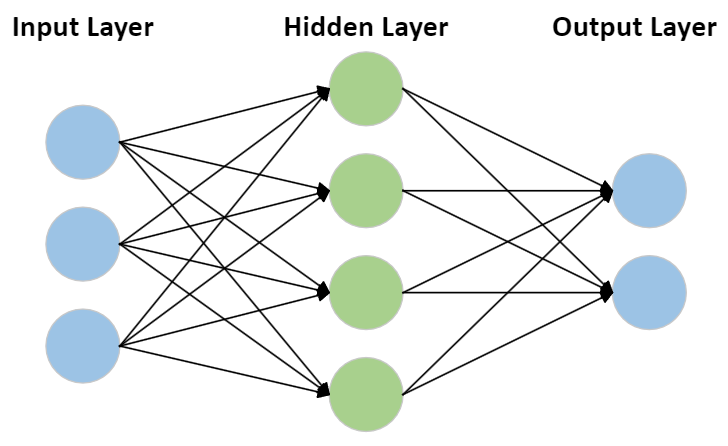
\includegraphics[width=0.55\linewidth]{graphics/Neural_Network.png}}
    \caption{figure of a neural network}
\end{figure}
Although, when these interconnected layers are stacked on top of each other, so multiple hidden layers are stacked on top of each other, the network is called deep.\footcite[cf.][305]{cichyDeepNeuralNetworks2019}
In general, deep learning methods can be seen as subset of machine learning methods and are today's fundament of artificial intelligence allowing to solve more complex tasks.\footcite[cf.][1583]{durstewitzDeepNeuralNetworks2019}
\ac{DNN}s are constantly growing and currently have around 1200 interconnected layers that equal to more than 16 million neurons inside a network .\footcite[cf.][2]{mallComprehensiveReviewDeep2023}
An example of a deep neural network is presented in figure 2 which shows the stacked layers in the middle of the network.
\begin{figure}[H]
    \centering
    \fbox{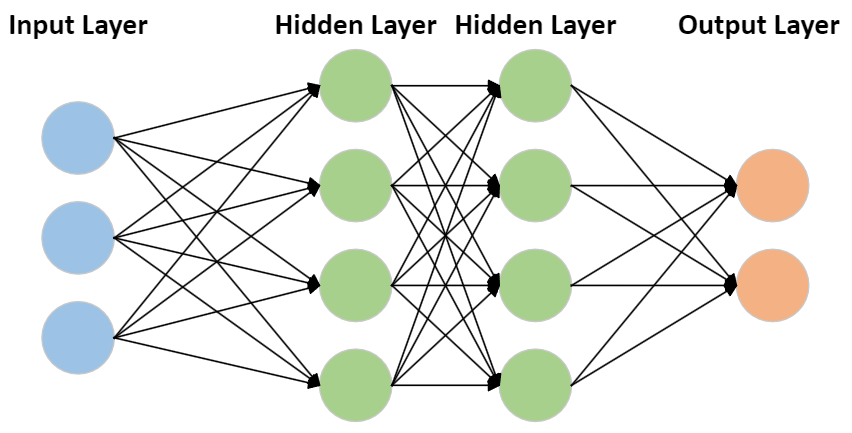
\includegraphics[width=0.6\linewidth]{graphics/Deep_Neural_Network_2.png}}
    \caption{figure of a neural network}
\end{figure}

Some examples for regression tasks within a \ac{DNN} in the field of acomputer vision include object detection, medical image registration, head- and body-pose estimation, age estimation and visual tracking.\footcite[cf.][325-326]{gustafssonEnergyBasedModelsDeep2020}
Nowadays, verly large neural networks with millions of parameters can be created due to the research achievements made in the field of neural networks and deep learning leading to highly performing models.\footcite[cf.][152]{marinoDeepNeuralNetworks2023}
Nonetheless, such models often have a negative effect on the environment in terms of unnecessary energy consumption and a limitation to their deployment on low-resource devices because they are excessively oversized and redundant.\footcite[cf.][152]{marinoDeepNeuralNetworks2023}


\subsection{Energy-based models}

An \ac{EBM} is a type of neural network that has special characteristics. 
One characteristic is that an \ac{EBM} is a statistical model.\footcite[cf.][2]{huembeliPhysicsEnergybasedModels2022}
This probabilistic approach willingly uses uncertainty into the model calculations to draw the models inputs randomly from its underlying distribution.\footcite[cf.][25-27]{uusitaloOverviewMethodsEvaluate2015}
This is done because the conventional deterministic method of backpropagation is known to potentially convert to local minimas, and requires long computation time.\footcite[cf.][109]{spechtProbabilisticNeuralNetworks1990}
As a result with conventional backpropagation more frequently incorrect classification would take place.
The second characteristic is that an \ac{EBM} is determined by an energy function that needs to be minimized in order to find the solution of the optimization problem.\footnote{cf.\cite{huembeliPhysicsEnergybasedModels2022}, p. 2; cf.\cite{ranzatoEfficientLearningSparse2006}, p. 1}
Since 1982, those statistical neural network models have been continuously emerging in the machine learning field when J.J. Hopfield introduced the Hopfield Network.\footcite[cf.][]{hopfieldNeuralNetworksPhysical1982}
Current developments include their use in reinforcement learning, potential replacements for discriminators in generative adversarial networks and for quantum \ac{EBM}s.\footnote{cf.\cite{verdonQuantumHamiltonianBasedModels2019}, p. 1; cf.\cite{duModelBasedPlanning2021}, p. 1}
In addition to that, Open AI showed that \ac{EBM}s are useful models across a wide variety of tasks like achieving state-of-the-art out-of-distribution classification and continual online class learning to name a few.\footcite[cf.][1-2]{duImplicitGenerationGeneralization2020}
The underlying idea behind \ac{EBM}s is to establish a probabilistic physical system that is able to learn and memorize patterns but most importantly generalize it.\footcite[cf.][2]{huembeliPhysicsEnergybasedModels2022} 
Especially, it involes learning an energy function \(E_{\theta}(x) \in \mathbb{R}\), with \( x \) representing the configuration of the network, and assigning the low energy to observed data \(x_i\) and high energy to other values \(x\).\footcite[cf.][330]{gustafssonEnergyBasedModelsDeep2020}
\begin{figure}[H]
    \centering
    \fbox{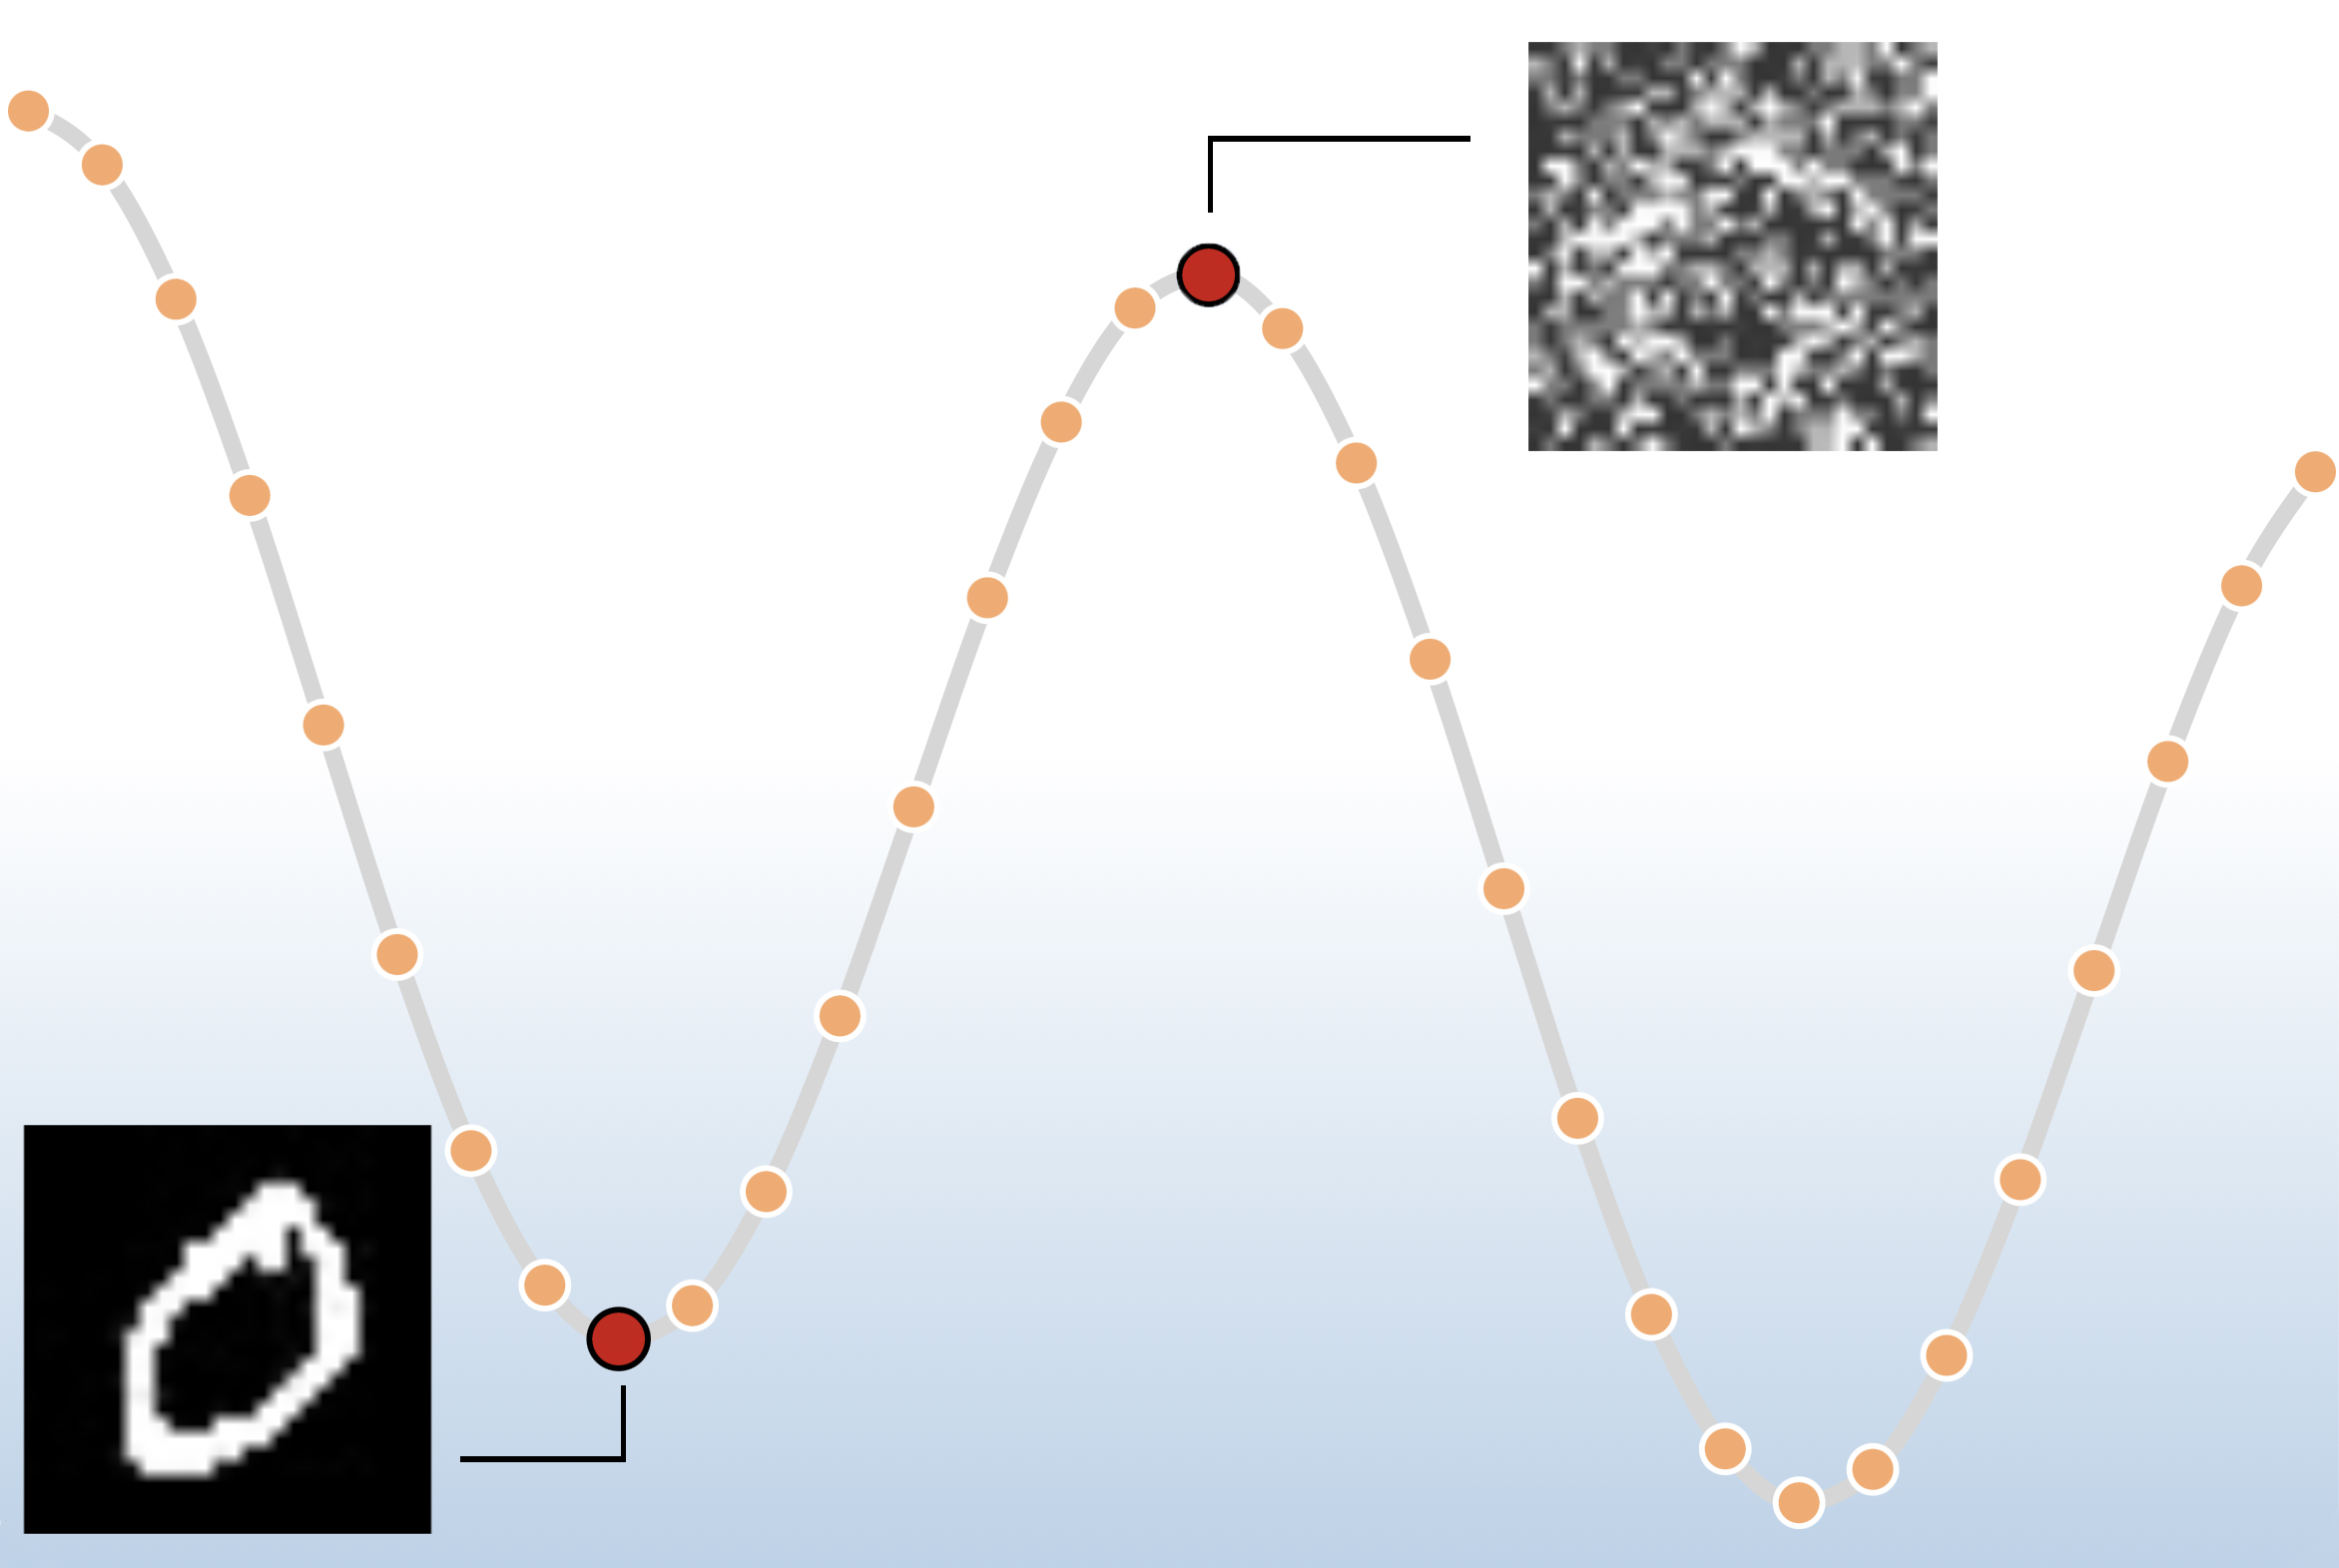
\includegraphics[width=0.4\linewidth]{graphics/energielandschaft.jpg}}
    \caption{Figure of a simplified energy landscape}
\end{figure}
In this figure 1 a simplified energy landscape is shown where the local minima corresponds to states that encode an MNIST digit.\footcite[cf.][6]{huembeliPhysicsEnergybasedModels2022} It is visible that observed data settles in the local minimum of the energy landscape, in this case a clear 0. On the other hand close to the local maxima of the energy landscape the 0 is only barely recognizable and therefore got a higher energy value assigned to it.
The assumption of the underlying distribution function \( P(x) \) represents the probability distribution over the input data x,
indicating how likely different configurations of x are under the models learned patterns:
\begin{equation}
    P(x) = \frac{1}{Z} \exp\left(-\frac{E(x)}{T}\right),
\end{equation}
where \( Z \) is the partition function to ensure
that the density function normalizes to a total probability of 1 and \( T \) is interpreted as the temperature.\footcite[cf.][2-3]{huembeliPhysicsEnergybasedModels2022}
The partition function \( Z \) used in 2.1 is given by summing over all possible pairs of visible and hidden vectors\footcite[cf.][4]{hintonPracticalGuideTraining2012}:
\begin{equation}
    Z = \sum_x \exp\left(-\frac{E(x)}{T}\right)
\end{equation}
The aim of the training in an \ac{EBM} is to match the true probability distribution \( P_{\text{data}} \) as closely as possible with the internal probability distribution \( P_{\text{model}} \) learned by the model.
What this means is that the specific aim is to adjust its parameters such that \( P_{\text{model}} \)
becomes as close to \( P_{\text{data}} \) as possible, which shows the model has learned the distribution of the real world data.
A practical method to achieve this goal is to use the KL divergence. KL divergence is a mathematical meassure that helps to meassure how close the predictions are by comparing the model's learned distribution to the true distribution of the data:
\begin{equation}
    G = \sum_x P_{\text{data}}(x) \ln \left( \frac{P_{\text{data}}(x)}{P_{\text{model}}(x)} \right)
\end{equation}
Here, \( P_{\text{data}} \) is the probability distribution when the network receives a speicific data input from the environmnet, while \( P_{\text{model}} \) represents the internal network running freely, also referred to as ``dreaming''.\footcite[cf.][154-155]{ackleyLearningAlgorithmBoltzmann1985}
In the training process the asymmetric divergence \( G \) needs to be miminized and therefore the probabiliies of the model converge close to the ones in reality.
To optimise the KL divergence the energy is adjusted, whereby data is assigned to low energy states (according to 2.1) and the training data receives high energy and therefore low probabiliies.\footcite[cf.][2-3]{zhaiDeepStructuredEnergy2016}

NACH UNTEN
As a side note it is worth mentioning that using the maximum likelihood estimator for \( Z \) is intractable due to the requirement of summing over all possible states, which leads to an exponential increase in the number of states for larger systems.\footcite[cf.][2-3]{zhaiDeepStructuredEnergy2016}

\subsection{concept of Boltzmann Maschines}

A \ac{BM} is a type of symmetrical \ac{EBM} consisting of binary neurons \{0, 1\}.\footcite[cf.][260]{amariInformationGeometryBoltzmann1992}
The neurons of the network can be split into two functional groups, a set of visible neurons and a set of hidden neurons.\footcite[cf.][154]{ackleyLearningAlgorithmBoltzmann1985}
Therefore, the \ac{BM} is a two-layer model with a visible layer (``v'') and a hidden layer (``h'').\footcite[cf.][448]{salakhutdinovDeepBoltzmannMachines2009}
The visible layer is the interface between the network and the environment. It receives data inputs during training and sets the state of a neuron to either \{0, 1\} which represents activated or not activated.
On the other hand, the hidden units are not connected to the environment and can be used to explain underlying constraints in the internal model of input vectors and they cannot be represented by pairwise constraints.\footcite[cf.][154]{ackleyLearningAlgorithmBoltzmann1985}
The connection between the individual neurons is referred to as bidirectional, as each neuron communicates with each other in both directions.\footcite[cf.][149]{ackleyLearningAlgorithmBoltzmann1985}
As early as 1985, one of the founding fathers of artificial intelligence, Geoffrey Hinton, was aware that an \ac{BM} is able to learn its underlying features by looking at data from a domain and developing a generative internal model.\footcite[cf.][148]{ackleyLearningAlgorithmBoltzmann1985}

Most machine learning models can be categorized in either generative or discriminative models. Both are strategies to estimate a probability that an specific object can be assigned to a category.\footcite[cf.][1]{hsuEffectsGenerativeDiscriminative2010}
Discrimivative models estimate the probability distribution based on category labels that are given to specific objects.\footcite[cf.][2]{gmComprehensiveSurveyAnalysis2020}
On the other hand, a generative model differ as follows. 
They generate a probabilistic model of the underyling probability distribution for each category, which is assumed as the basis of the data, and in a following step they use Baye's rule to identify which category is very likely to have establihed the object.\footcite[cf.][1]{hsuEffectsGenerativeDiscriminative2010}
An real world example would be the following: to predict if a movie will be a hit, you could analyze past box office successes to model characteristics shared by hits (generative approach), or assess immediate audience reactions to movie trailers and reviews to predict success without modeling historical data (discriminative approach).
Therefore it can be said that \ac{BM}s and \ac{EBM}s are generative models. In the following figure \ref{fig1}, a general \ac{BM} is depicted, where the upper layer embodies a vector of stochastic binary 'hidden' features, while the lower layer embodies a vector of stochastic binary 'visible' variables.\footcite[cf.][449]{salakhutdinovDeepBoltzmannMachines2009}

\begin{figure}[H]
    \centering
    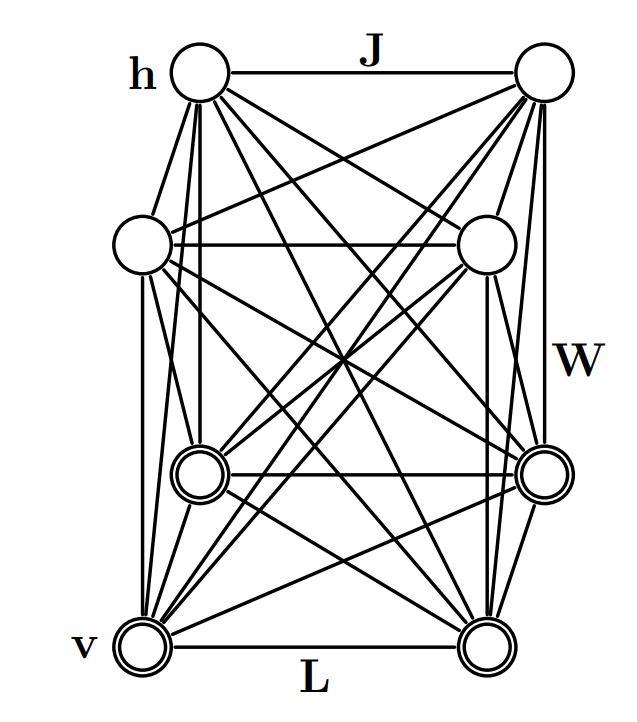
\includegraphics[width=0.25\linewidth]{graphics/General_BM.png}
    \caption{figure of a general Boltzmann Machine}
    \label{fig1}
\end{figure}
The model contains a set of visible units \( v \in \{0, 1\} \), and a set of hidden units \( h \in \{0, 1\} \) (see Fig. 1). The energy function of the \ac{BM} with the states \( \{v, h\} \) is defined as:
\begin{equation}
E(v, h; \theta) = -\frac{1}{2} v^T L v - \frac{1}{2} h^T J h - v^T W h,
\end{equation}

where \( \theta = \{W, L, J\} \) are the model parameters.\footcite[cf.][448]{salakhutdinovDeepBoltzmannMachines2009}
\( W, L, J \) represent visible-to-hidden, visible-to-visible and hidden-to-hidden weights.
In \ac{BM} each neurons works towards minimizing the global energy by 
entering a particular neuron configuration representing a input to the machine and the system will find the minimum energy configuration that is compatible with the given input.\footcite[cf.][150]{ackleyLearningAlgorithmBoltzmann1985}
A simple method to find a local energy minimum involes to switch into wichever of the two states (on or off) of a neuron result in a lower energy given the current state of the other neurons.\footcite[cf.][110]{fahlmanMassivelyParallelArchitectures1983}    
Integrating the function 2.4 into the earlier introduced KL-divergence 2.2 and doing gradient descend a learning rule to update the weights and biases appers.\footcite[cf.][5]{hintonPracticalGuideTraining2012}
The gradient descent algorithm is commonly used in machine learning and is an iterative technique that adjusts the model parameters (weights and biases).\footcite[cf.][11]{wangResearchApplicationGradient2021}
It progressively acquires the gradient of the energy function, methodically advancing towards the optimal solution and ultimately achieves the minimum loss function along with adjusted parameters.\footcite[cf.][11]{wangResearchApplicationGradient2021}
Consequently, this leads to the specific learning rule\footcite[cf.][5]{hintonPracticalGuideTraining2012}:
\begin{equation}
    \Delta w_{ij} = \epsilon ( \langle v_i h_j \rangle_{\text{data}} - \langle v_i h_j \rangle_{\text{model}} )
\end{equation}

The network can now update the weights ``W'' that exist between the neurons through the training rule based on the observations that served as input. \footcite[cf.][1-2]{barraEquivalenceHopfieldNetworks2012}
In this case, the square brackets represent expected values, as the training is based on the activation probability.
In addition to that, the step sizes of updates to the weights are influenced by the learning rate \(\epsilon\) within the iterative training process.

Performing exact training in this model is intractable because exact computation of the data predictions and the model predictions takes a time that is exponential in the number of hidden units.\footcite[cf.][449]{salakhutdinovDeepBoltzmannMachines2009}
When the number of hidden units is large compared to the number of visible units it is impossible to achieve a perfect model because of the totally connected network and the resulting \( 2^n \) possbilities.\footcite[cf.][154]{ackleyLearningAlgorithmBoltzmann1985}
Hereby, \( n\) represents the number of neurons in the network with each neuron being in one of the two states, the total sum of possibilities are \( 2^n \).
This leads back to the briefly mentioned constraint of equation 2.3, that is needed to calculate an activation probability of a neuron, which is required to update a weight in the training process shown in 2.5.

A specific example to demonstrate why it is intractable to calculate an activiation of a \ac{BM} is the following. A fictional \ac{BM} has 80 visible nodes and 120 hidden nodes and therefore the possbilities of states of neurons are \( 2^{200} \), which is \( 1.61 \times 10^{60}\). 
To put this into perspective, the total atoms that exist on earth are only estimated to be around \( 1.33 \times 10^{50}\).\footnote{cf.\cite{helmenstineHowManyAtoms2022}, p. 478-480; cf.\cite{schlammingerCoolWayMeasure2014}, p. 1}
That means even if it would be possible to store one information per atom it would just not be enough. 

As a result, instead of directly trying to train the model sampling methods are used that are able to estimate these activation probabiliies.
This enables the training of \ac{BM}s and \ac{RBM}s.
\subsection{Restriced Boltzmann Machines}

As a simplification of the training problem Hinton and Sejnowski proposed Gibbs sampling as an algorithm to aporoximate both expectations.\footcite[cf.][158-165]{ackleyLearningAlgorithmBoltzmann1985}
Furthermore, the intralayer connections of the model got removed and the result is the so called \ac{RBM}.
To transform an \ac{BM} into a \ac{RBM} the diagonal elements \( L \) and \( J \)  introduced earlier, are set to 0 and as a result the well-known model of a \ac{RBM} establishes shown in fig.5.\footcite[cf.][449]{salakhutdinovDeepBoltzmannMachines2009}

\begin{figure}[H]
    \centering
    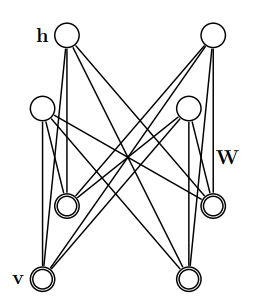
\includegraphics[width=0.25\linewidth]{graphics/RBM_Modell.png}
    \caption{Figure of a \ac{RBM}}
\end{figure}
What can be recognized that no more visible-to-visible and hidden-to-hidden connections can be found in the model.
The configuration of the visible and hidden units \( (v, h) \) therefore has also an updated energy function (Hopfield, 1982) given by:
\begin{equation}
E(v, h) = - \sum_{i \in \text{visible}} a_i v_i - \sum_{j \in \text{hidden}} b_j h_j - \sum_{i,j} v_i h_j w_{ij},
\end{equation}
where \( v_i, h_j \) are the binary states of a visible unit \( i \) and hidden unit \( j \), \( a_i \) and  \(  b_j \) are their biases and \( w_{ij} \) is the weight between them.\footcite[cf.][3-4]{hintonPracticalGuideTraining2012a}
Despite, compared to the fully connected \ac{BM}, the \ac{RBM} is less complex but the advantages of training surpasses the loss in expressivity possibilities.\footcite[cf.][4]{huembeliPhysicsEnergybasedModels2022}
The \ac{RBM} has recently been drawing attention in the machine learning community beceause of its adaption and extention for various tasks such as representational learning, document modeling, image recognition and for
serving as foundational components for deep networks including Deep Boltzmann Machines, Deep Belief Networks and hybrid models with CNNs.\footcite[cf.][1186]{zhangOverviewRestrictedBoltzmann2018}

\subsubsection{Training of \ac{RBM}s}

The training of \ac{RBM}s can be established with the use of sampling methods that estimate the activation probabilities, which are needed to update the weights.
There are currently two methods that can be chosen from: contrastive divergence and the Metropolis-Hastings algorithm. 
The goal of the techniques is to create a sequence of correlated steps from a random walk that, after enough iterations, makes it possible to sample a desired target probability distribution.\footcite[cf.][1]{patronOptimalRelaxationRate2024}
In the following part both methods will be explained in depth.
Especially, they are interesting since they serve as baselines to compare against the new sampling method of a hopfield network that is to be achieved in the practical part of the thesis.

\textbf{Contrastive Divergence:} Contrastive divergence is a special Gibbs Sampling training method
developed by Geoffrey Hinton for the efficient training of \ac{RBM}s.\footcite[cf.][4-5]{hintonPracticalGuideTraining2012}
In traditional, Gibbs sampling would have to generate a long chain of samples, until
independent samples are obtained from the observed data distribution of the model.\footcite[cf.][5-6]{huembeliPhysicsEnergybasedModels2022}
The samples are needed for each iteration of the gradient ascent on the log-likelihood
resulting in large computational costs.\footcite[cf.][7-8]{upadhyaOverviewRestrictedBoltzmann2019}
To solve this issue contrastive divergence minimizes an approximation of the Kullback-Leibler divergence between the empirical distribution of the training data and the distribution generated by the model.\footcite[cf.][246]{mocanuTopologicalInsightRestricted2016}
They way to achieve this is by initializing the Markov chain with the samples from the data distributon.\footcite[cf.][7-8]{upadhyaOverviewRestrictedBoltzmann2019}
The outcome has been shown to heavily decrease the training time while only adding a small bias.\footcite[cf.][537]{larochelleClassificationUsingDiscriminative2008}
This allows to calculate the probabilities of equation 2.5. 
This entails initializing the visible units using an actual data input, such as an MNIST sample, and then commencing the subsequent steps with the hidden states.
Often the process can be stopped after only sampling a very small number of steps.\footcite[cf.][646]{larochelleLearningAlgorithmsClassification2012}


\textbf{1. Forward Pass (positive phase)}

During the forward pass using the Gibbs Sampling method, the visible units are set to a completely random state. Next up the hidden units are computed.
The computation of the hidden units involves calculating their activation probabilities and performing an actual sampling with their calculated activation probabilities.
With the \ac{RBM} it is now easy to get an analytical calculated sample of $(\textbf{v}_i\textbf{h}_j)_{data}$.\footcite[cf.][5]{hintonPracticalGuideTraining2012}
Given an input data out of the training images, \( v \), the binary state, \( j \), of each hidden unit,  \( h_j \), is set to 1 with following probability:

\begin{equation}
p(h_j = 1 | \textbf{v}) = \sigma(b_j + \sum_i v_i w_{ij}),
\end{equation}
where $\sigma(x)$ is the logistic sigmoid function with an unbiased sample. The sigmoid function is defined as $\sigma(x) = \frac{1}{1 + \exp(-x)}$ and is needed because it is the underlying activation function of each neuron.
A visual representation is shown in figure 6:
\begin{figure}[H]
    \centering
    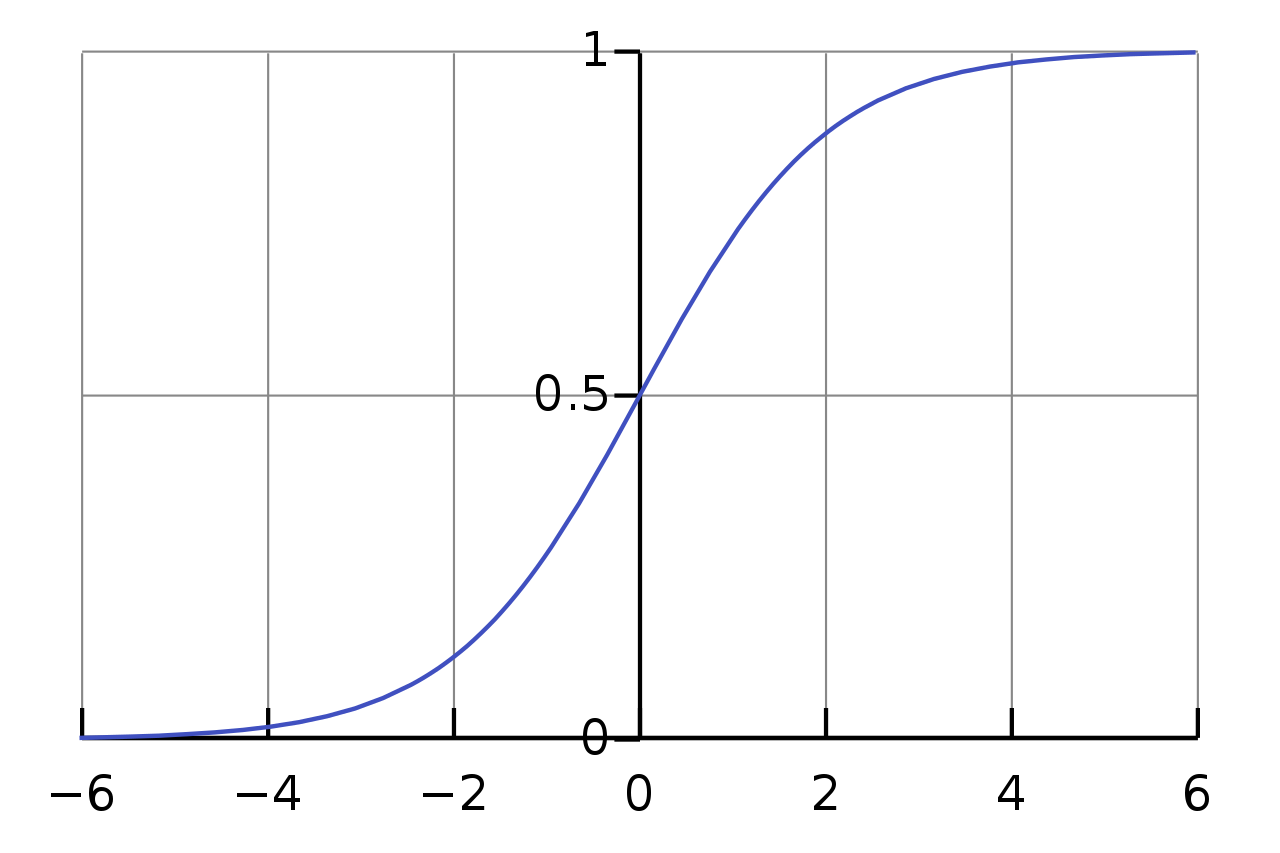
\includegraphics[width=0.5\linewidth]{graphics/logistic_sigmoid.png}
    \caption{Figure of a logistic sigmoid function \ac{RBM}}
\end{figure}
The result is a set of probabilities that reflect how likely it is for each hidden unit to be on, wich stands for \( 1 \), or, which stands for \( 0 \), given the input data.\footcite[cf.][6]{huembeliPhysicsEnergybasedModels2022}
The sampling part of the positive phase uses the just calculated activation probabiliy of each hidden unit and performs a random experiment with it.
That random experiment generates a uniform random number between 1 and 0 and if the random number is greater than the just calculated activiation probability the hidden unit is set to activated.
Afterwards, the hidden unit is either activated or not activated and the training process continues with the new state of the hidden units.

\textbf{2. Reconstruction (negative phase)}

In this phase, the sampled hidden states are used to reconstruct the visible units. 
This is essentially a prediction of the input, which is how the model sees the input based on the just updated hidden units and is calulated with following probability:\footcite[cf.][6]{hintonPracticalGuideTraining2012}
\begin{equation}
    p(v_i = 1 | \mathbf{h}) = \sigma(a_i + \sum_j h_j w_{ij})
\end{equation}
The sampling part of the negative phase uses the just calculated activation probabiliy
of each visible unit and performs a random experiment, like in the positive phase.
Now, the result is a prediction of the input in the visible nodes.
Afterwards, a half forward pass is made to calculate the activation probability of a hidden unit again based on the activated or not activated visible units.

\textbf{3. Updating the weights}

Now, all the requirements to update the weights are satisfied and can be used within the equation 2.5. 
The delta that results is summed to the current weight and the internal model gets closer to prediciting the observed data.
In total, one training iteration consists out of 1 Forward Pass, 1 Reconstruction and 0.5 Forward Pass again is accomplished.
Repeating this training steps \( N \) times for a suitable chosen \( N \) the model learns better, since more steps of alternating Gibbs sampling were performed.\footcite[cf.][6]{huembeliPhysicsEnergybasedModels2022}


\textbf{Metropolis-Hastings:} The Metropolis-Hastings algorithm, often only called Metropolis algorithm, is a technique out of \ac{MCMC} class techniques.\footcite[cf.][1]{patronOptimalRelaxationRate2024}
The Metropolis-Hastings method was invented by Metropolis et al. in 1953 when they noticed, that for an intractable distribution with too many states it can be seen as a limiting distribution of Markov chains.\footcite[cf.][1087-1092]{metropolisEquationStateCalculations1953} 
The intractable distribution to handle with the Metropolis-Hastings technique in the case of \ac{RBM}s is equation 2.3.
An Interpretation of the method can be expressed as: "A visitor to a museum that is forced by a general blackout to watch
a painting with a small torch.
Due to the narrow beam of the torch, the person cannot get a global view of the painting but can proceed along this painting until all parts have been seen."\footcite[cf.][2]{robertMetropolisHastingsAlgorithm2016}
The version already adjusted for \ac{RBM}s incorporates the following functionality of the Metropolis technique:

First, select a random or given configuarion $x_{\text{old}}$ of a \ac{RBM} that holds the states of all visible and hidden neurons.\footcite[cf.][65]{beichlMetropolisAlgorithm2000}
Secondly, the energy of the configuration, noted as  $E_{\text{old}}$, must be calculated using Equation 2.6, as previously introduced. Subsequently, this energy value is stored.
Thirdly, the configuration gets updated by picking one random neuron and changing the state of it from 0 to 1 or vice versa.\footcite[cf.][1]{rosenthalOptimalProposalDistributions2009}
This new configuration is stored as $x_{\text{new}}$. Following that the energy of the new configuration $E_{\text{new}}$ is calculated and stored.
Now the two energy values are compared and if $E_{\text{new}}$ <= $E_{\text{old}}$ the new configuration will be accepted and $x_{\text{old}}$ = $x_{\text{new}}$.\footcite[cf.][1-2]{patronOptimalRelaxationRate2024}
If $E_{\text{new}}$ > $E_{\text{old}}$ then there are some extra steps to be followed: 

The flip probability is calculated as $p=\exp\left(-\frac{E_{\text{new}}-E_{\text{old}}}{kT}\right)$.
\( KT \) is interpreted as the temperature in the network and with higher temperature it increases
the activation probability leading to an faster exploration through the landscape but with less details.\footcite[cf.][1-9]{liTemperatureBasedRestricted2016}
For \ac{RBM}s \( KT \) is assumed to be 1.\footcite[cf.][3]{hintonBoltzmannMachines2014} In the following figure 7 the resulting probability function is shown.

\begin{figure}[H]
    \centering
    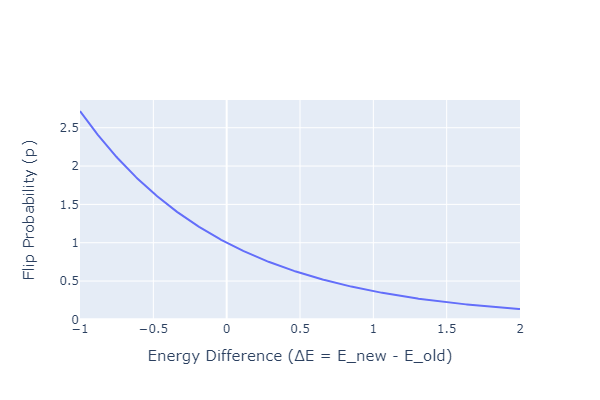
\includegraphics[width=0.7\linewidth]{graphics/Flip Probability Function in Metropolis-Hastings Algorithm2.png}
    \caption{Flip Probability Function in Metropolis-Hastings Algorithm}
\end{figure}

In the next step a uniform random number $r$ between 0 and 1 is generated.
After generating $r$ the configuration will be accepted if $r \leq p$ (i.e., $x_{\text{old}}=x_{\text{new}}$).\footcite[cf.][2-3]{patronOptimalRelaxationRate2024}
Otherwise, a rejection takes place if $r > P$ (i.e., $x_{\text{old}}=x_{\text{old}}$).

Finally, the configuration $x_{\text{old}}$ can be stored and the process repeats beginning from step 2 on.\footcite[cf.][17]{patronOptimalRelaxationRate2024}
After repeating enough times the activation probability for each neuron can be calculated by summing over all samples $(x_1+x_2+x_3+\ldots)$ and the result is divided by the total number of samples.

\subsection{Current Problems witht BMs and RBMs}

One general problem that occurs in the learning process of a \ac{BM} is that it is both time-consuming and difficult.\footcite[cf.][1-2]{fischerIntroductionRestrictedBoltzmann2012}
This is because sampling from an undirected graphical model is not straightforward and therefore \ac{RBM}s make use
of \ac{MCMC} proposed methods like Contrastive Divergence and Metropolis Hastings.\footcite[cf.][2]{fischerIntroductionRestrictedBoltzmann2012}
In addition to that, the selection of hyperparameters can be difficult since for the training of a practical model a large hyper-parameter space needs to be explored.\footcite[cf.][536]{larochelleClassificationUsingDiscriminative2008}
Hyperparmeters are: the learning rate, size of the hidden layer, number of training iterations iteration count per bias (sampling step size), initializing the weight sizes in the beginning but also the method for calculating activation probabilities (Contrastive Divergence, Metropolis Hastings, etc.).
As a result, establishing a \ac{RBM} with perfect hyperparameters is time consuming and can be seen as art.
Furthermore, training can become unstable and predictions become inaccurate due to an incompatible selected temperature.\footcite[cf.][3-4]{huembeliPhysicsEnergybasedModels2022}
A lower temperature reduces the system's possbility to explore the energy landscape thoroughly, leading to the false selection of local minima instead of finding the global minimum.
Vice versa a too high temperature can cause that the energy landscape is not explored enough and has gaps between it missing some minima or skipping the global maxima. 
Luckily, the temperature for \ac{RBM}s is expected to be \( 1 \) and only for specific use cases it makes sense to adjust internal temperature.

To accelerate the training process of a \ac{RBM}, it is crucial to address the most computationally demanding aspect: the matrix-vector multiplication involved in the sampling process.
A possbilty of achieving this is using dedicated hardware, so called hardware accelerators for this problem. 
They are designed to tackle a specific task very efficiently, like matrix vector multiplications, which are widely used within most of the neural networks.\footcite[cf.][3881-3882]{lehnertMostResourceEfficient2023}
That is the reason why they are significant for the acceleration of this thesis and an interesting technology to look at.  


\section{Hardware accelerators}
\subsection{Current approaches in the field of AI and other solutions}
Since Neural Networks and \ac{DNN}s are growing their parameters at rapid rates they constantly achieve better and better resutls and are able to solv even more complex tasks.\footcite[cf.][1]{baischerLearningHardwareTutorial2021}
This upcoming trend of growing network sizes exponentially also brings a dark side with it: An excessive increase in computational effort and memory size.\footcite[cf.][1-2]{baischerLearningHardwareTutorial2021}
As a result \ac{CPU}s can barely satisfy the required performance and specialized hardware accelerators are used to increase the performance of these Neural Networks.\footnote{cf.\cite{zhouPhotonicMatrixMultiplication2022}, p. 1-2; cf.\cite{baischerLearningHardwareTutorial2021}, p. 2}
In addition to that for many use cases, like autonomous driving, there are high energy, latency, and runtime predictability constraints \ac{CPU}s are not able to meet.\footcite[cf.][2692]{ahmadOptimizingHardwareAccelerated2020}

The concept of developing hardware accelerators is not new.
However, their limited adoption and the fast obsolescence of even the most outstanding accelerators have made the investment in them uneconomical compared to general-purpose processors that surpassed them.\footcite[cf.][2]{peccerilloSurveyHardwareAccelerators2022}
At present, however they are seen as promising driving force of computer architecture since they are the optimal solution to satisfy the growing computation-hungry demands of businesses, especially within machine learning workloads.\footcite[cf.][2-3]{peccerilloSurveyHardwareAccelerators2022}
An hardware accelerator can be defined as "a separate architectural substructure that is architected using a different set of objectives than the base processor, where these objectives are derived from the needs of a special class of applications".\footcite[cf.][2]{peccerilloSurveyHardwareAccelerators2022}
Broken down, they are specialized hardware, expertly optimized for the unique demands of certain application categories, freeing them from the restrictions usually placed on general-purpose processors.
Moreover, a hardware accelerator doesn't replace the conventional processor, which is still used for the operating system, it rather enables specific workloads to be executed on it very efficiently.\footcite[cf.][2-3]{peccerilloSurveyHardwareAccelerators2022}
There are different approches such as \ac{GPU}s, \ac{ASIC}s, \ac{FPGA}s, but also new approaches like Quantum Computations or Photonic matrix multiplication are researched.\footnote{\cite{zhouPhotonicMatrixMultiplication2022}, p. 1-2; cf.\cite{baischerLearningHardwareTutorial2021}, p. 2}
All of these methods have different use cases and get more and more application specific. The list of the sequence, sorted by application-unspecific to specific for established approches looks the following:
\[
\text{CPU} \xrightarrow{\text{less flexible}} \text{GPU} \xrightarrow{\text{specialized}} \text{FPGA} \xrightarrow{\text{more customized}} \text{ASIC}
\]
Currently the approaches can be segmented into three categories:
\textbf{Firstly}, the design of data-driven digital circuits.
It consists the shift from general-purpose GPUs to specialized dataflow architectures like systolic arrays, which are used in Google’s Tensor Processing Units (TPUs).
These architectures are noted for their efficiency in performing deep learning operations by reducing control hardware and keeping data movement local.\footcite[cf.][3883]{lehnertMostResourceEfficient2023}
\textbf{Secondly}, network structure optimizations. 
Hereby modifications to the neural networks themselves are made to improve hardware efficiency.
One method is quantization, which simplifies arithmetic operations and reduces memory needs by using fixed-point representations of data and weights instad of using for example 32-bit floating points.
The other one is pruning, which involves setting certain weights to zero to reduce the complexity of operations.\footcite[cf.][3883]{lehnertMostResourceEfficient2023}
\textbf{Thirdly}, technology-driven designs.
Current research into using novel circuitry and memory cells include memristive memory cells and silicon photonics, to further enhance performance and energy efficiency.
They work by storing the network weights and calculating the vector multiplications with analaog signals with technologies like crossbar arrays.
While these technologies promise significant advantages, their practical application is still being explored.\footcite[cf.][3883]{lehnertMostResourceEfficient2023}
The following three accelerator approaches can be categorized into the first category:

\subsection{GPU}
The \ac{GPU}, is by far the most common accelerator in the market with a focus at computational-complex workloads.
Also \ac{GPU}s enabled great achievements in \ac{DNN}s due to their massive parallelization potential of computations and their high troughputs compared to \ac{FPGA}s and \ac{ASIC}s.\footcite[cf.][16]{baischerLearningHardwareTutorial2021}
A \ac{GPU} is a manycore unit that features up to hundreds of multi-processors that consist of in-order cores which are able to exploit massive threadlevel parallelism.\footcite[cf.][2]{peccerilloSurveyHardwareAccelerators2022}
They excel at performing numerous floating-point arithmetic operations for vector processing on large datasets with high degrees of data-parallelism.
In practice this works by breaking down workloads into small tasks that can be processed by the enormous amount of cores in parallel.\footcite[cf.][101]{huSurveyConvolutionalNeural2022} 
With development of real-time graphics \ac{GPU}s became programmable too. The combination of programmability and floating-point performance
make them very attractice for machine learning workloads and is the reson for their dominance in the market.\footcite[cf.][42]{dallyEvolutionGraphicsProcessing2021}
On top of that, the widespread adoption of \ac{GPU}s has led to extensive support across numerous frameworks and high-level APIs commonly used in Machine Learning.\footcite[cf.][16]{baischerLearningHardwareTutorial2021}
Well-known frameworks would be PyTorch or TensorFlow.
However, compared to the other two accelerator apporaches the \ac{GPU} is not as flexible and has higher latency and energy consumption.\footcite[cf.][100]{huSurveyConvolutionalNeural2022}

\subsection{Field programmable gate arrays}
In contrast, \ac{FPGA}s have also demonstrated enormous parallelization capabilities due to their fast digital signal processors and on-chip
memory which result in lower energy cost than GPUs.\footcite[cf.][2693]{ahmadOptimizingHardwareAccelerated2020}
They work by using reconfigurable logic blocks that can be interconnected using routing tracks with configurable switches at the intersections.\footcite[cf.][144]{babuReconfigurableFPGAArchitectures2021}
This combined with the use of many digital signal processors and local storage of data in the hardware enables the development of the exact hardware needed for a workload.\footcite[cf.][19]{baischerLearningHardwareTutorial2021}
As a side note it is worth mentioning that the most energy-consuming task of a workload is the data transfer and not the computation iself.
In the context of \ac{FPGA}s, they use their on-chip memory to reduce the data transfer significantly and therefore achieve a sweet spot between computation speed and energy efficiency.\footcite[cf.][101-102]{huSurveyConvolutionalNeural2022}
Hence, they are utilized to design a specialized processor tailored for executing specific workloads, like machine learning, effectively.\footcite[cf.][322]{sipolaArtificialIntelligenceIoT2022}
Furthermore, due to their reprogrammable nature they have a lower engineering cost and faster time-to-market compared to \ac{ASIC}s.\footcite[cf.][4]{boutrosFPGAArchitecturePrinciples2021}
With \ac{FPGA}s the implementation time could only be a matter of weeks and also allows to support continious upgrades and bug fixes even after the deployment which is not possible within \ac{ASIC}s\footcite[cf.][4]{boutrosFPGAArchitecturePrinciples2021}
Even though the \ac{FPGA} possesses all these advantages with their high flexibility, latency and low energy consumption, they are sometimes inferior in throughput compared to a \ac{GPU}.\footcite[cf.][100]{huSurveyConvolutionalNeural2022}

\subsection{Application specific integrated circuit}
\ac{ASIC}s can be distinguished from \ac{FPGA}s because they are not programmable. 
In addition to that, they offer the highest degree of customization and are designed to execute a specific application with the utmost efficiency.\footcite[cf.][17]{baischerLearningHardwareTutorial2021}
So the attributes of \ac{ASIC}s are the focus on specific tasks and the strong design freedom.
Nowadays, the most common type of \ac{ASIC}s are \ac{TPU}s because of their matrix vector multiplications abilities that are needed within machine learning. But conventional \ac{ASIC}s work by mapping neurons directly to the hardware.\footcite[cf.][104]{huSurveyConvolutionalNeural2022}
Their design architecture enables them to outperform \ac{GPU}s and \ac{FPGA}s in terms of their small size, greater computation speed and high power efficiency.\footcite[cf.][17]{baischerLearningHardwareTutorial2021}
Specifically when compared to corresponding \ac{FPGA} circuits  \ac{ASIC}s are 35x smaller and 4x faster. 
A more current study could show that this gap is reduced but they still are 9x smaller and also faster.\footcite[cf.][5]{boutrosFPGAArchitecturePrinciples2021}

Nonetheless, developing an \ac{ASIC} requires expert knowledge in chip design but also within neural networks and takes a lot of time.\footcite[cf.][17]{baischerLearningHardwareTutorial2021}
Out of the three approaches, they provide the most efficient solution, yet it comes at the expense of lacking reconfigurability, no programmability, and incurring high engineering costs.\footnote{cf. \cite{peccerilloSurveyHardwareAccelerators2022}, p. 4; cf.\cite{huSurveyConvolutionalNeural2022}, p. 100}
With a sustainability and climate-change aspect in mind, they are the by far the best option since they represent the most power efficient approach with also the best computation speed.


\section{Memristor Hopfield Neural Network}

The so called \ac{mem-HNN} is a a hardware accelerator that uses an emerging approach of combining analog signals and electronical signals to solve complex optimization problems.\footcite[cf.][410]{caiPowerefficientCombinatorialOptimization2020}
It can be categorized into the \ac{ASIC} family of hardware accelerators and its specific purpose is to solve Ising problems. 
In 1925 Ernst Ising, a german physicist, invented the Ising model which explained the interaction between ferromagnets.\footcite[cf.][253-258]{isingBeitragZurTheorie1925}
This statistical model focuses on the state of a spin \( s_{i} \) (up and down; \( +1 \) and \( -1 \)) representing their mangetical behaviour. 
The Ising model calculates the total energy of a system though the following energy function: 
\begin{equation}
    E(\mathbf{s}) = \sum_{i } h_i s_i + \sum_{i,j} J_{ij}s_{i}s_{j}, \quad s_i = \pm 1,
\end{equation}
where \( i \) is the label of the spins \( s_{i} \), with \( h_{i} \) representing the external magetic field  interacting with each spin, and \( J_{ij} \) is the interaction strength between pairs of spins that are connected by an edge \( (ij) \).\footcite[cf.][2]{tanahashiApplicationIsingMachines2019}
Both values \( h_{i} \) and  \( J_{ij} \) are real-valued allowing for a wide range of possible magnetic field intensities and vary in interaction strength.\footcite[cf.][1-2]{wangOscillatorbasedIsingMachine2017}
Nowadays, the Ising modell is also attractive in other fields to describe the energy of a system and to transform them into an Ising problem.\footcite[cf.][2-3]{tanahashiApplicationIsingMachines2019}
Solving Ising problems is equal to finding the minimum energy state of a system.
Hence, in practice transforming optimzation probelms into Ising problems, the optimal solution is equal to the minima of the Ising energy function. 
This transformation works by mapping each variable of the problem to Ising spins and designing an Ising model whose ground state represents the solution.\footcite[cf.][2-3]{lucasIsingFormulationsMany2014}

Equivalence between the energy function of a \ac{mem-HNN} and the energy function of a \ac{RBM} can be shown here.
The energy function of the \ac{mem-HNN} works by using the binary states of \( +1 \) and \( -1 \) while the \ac{RBM} uses \( +1 \) and \( 0 \) but otherwise they are completely equal.
To transform the \ac{RBM} into the binary states of the \ac{mem-HNN}, its energy function from 2.6 needs to be modified with \(\frac{x + 1}{2}\) where \( x \) represents the energy function.
The fact, that both energy functions are equal implies that the neural network of a \ac{RBM} could possibly be trained on this Ising machine.
Moreover, other artificial intelligence models could be compatible but currently there are no apporaches on how to transform them.

Comming back to the Ising machine itself, the background for the development is the current slow down or failure of Moore's law which causes slow improving computation speed, energy efficiency and computation latency of conventional semiconductor electronical technology.\footcite[cf.][1]{caiHarnessingIntrinsicNoise2019}
Since the \ac{mem-HNN} is engineered to solve Ising problems, therefore also called Ising machine, it can tackle various problems that fall under the category of Ising problems.\footcite[cf.][363]{mohseniIsingMachinesHardware2022a}
Originally the mem-HNN was experimental tested by the team of researches to solve nondeterministic polynomial-time hard, or NP-hard for short, Ising problems directly on the hardware.\footcite[cf.][410]{caiPowerefficientCombinatorialOptimization2020}
NP-hard problems are amoung the toughest problems to solve and have an expontential- or even factioral time to solve (\( 2^{n} \), \( n{!} \)) with no efficient solution, slow to solve and to verify.\footcite[cf.][497-500]{izadkhahNPNPCompleteNPHard2022}
Well-known examples would be the salesman problem, the maximum clique problem or the calculation of the partition function of the \ac{BM} with \( 2^{n} \) possibilities.

In simple terms, this Ising machine is able to efficiently find the global minima of energy functions that are the underlying structure of an Ising problem. 
The name \ac{mem-HNN} already indicates that the Ising machine is based on the concept of a Hopfield Network.
All this is possible beause the update formula of the Hopfield Network is directly implemented on the hardware of the accelerator.
A photograph of the physical \ac{mem-HNN} accelerator (left side) and a microscopic view of it (right side) can be seen in following figure: 
\begin{figure}[H]
    \centering
    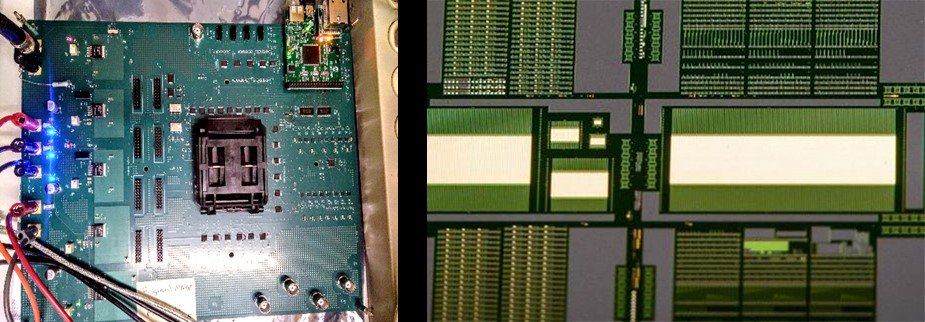
\includegraphics[width=0.65\linewidth]{graphics/Bilder_physische_beschleuniger.jpg}
    \caption{Physical and microscopic view of the mem-HNN}
\end{figure}
\subsection{Hopfield Network}

A Hopfield Network is an \ac{EBM} and belongs to the field of recurrent neural networks.\footcite[cf.][35]{dramschChapterOne702020}
Because the Hopfield Network is the underlying structure of the physical \ac{mem-HNN} accelerator this model is explained first.
The structure of the network consists of only one single layer with binary valued neurons inside.\footcite[cf.][7]{ahadNeuralNetworksWireless2016}
Therefore, the neurons state can either be \{1, 0\} or \{1, -1\}.
The connections between the neurons are symmetrical, which means that the weights of the connections are the same in either direction.\footcite[cf.][7]{ahadNeuralNetworksWireless2016}
Initially, the primary applications of this type of network were to serve as storage for associative patterns and to facilitate pattern retrieval.\footcite[cf.][2]{ramsauerHopfieldNetworksAll2021}
In practive given a query pattern a Hopfield Network can retrive a pattern that is most similar or an is an average of similar patterns.\footcite[cf.][2]{ramsauerHopfieldNetworksAll2021}
In this paper the Hopfield Network's update function interests us because it possibly could be used to sample the intractable training of a \ac{RBM} mentioned earlier.
Surprisingly, since Hopfield networks were introduced by J.J Hopfield in 1982 the storage capacity got increased over time but the fundamentals stayed the same.\footnote{cf.\cite{hopfieldNeuralNetworksPhysical1982}, p. 2554-2558; cf.\cite{ramsauerHopfieldNetworksAll2021}, p. 2}
In following figure 6 an example of a Hopfield Network can be seen.\footcite[cf.][1-2]{yaoMassivelyParallelAssociative2013}

\begin{figure}[H]
    \centering
    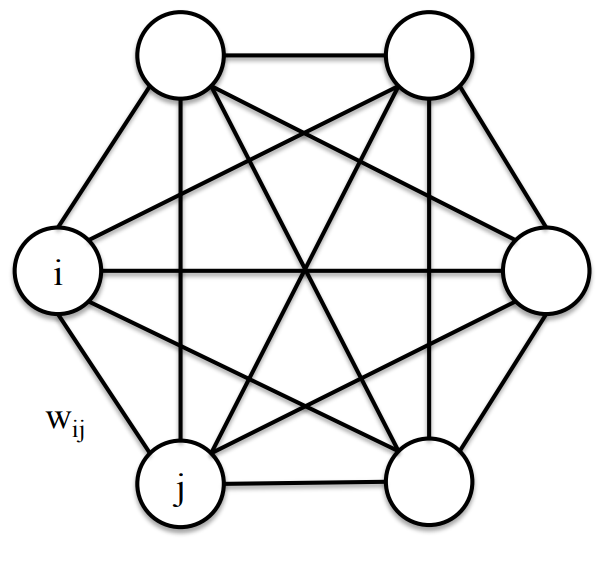
\includegraphics[width=0.3\linewidth]{graphics/Hopfield_Netzwerk.png}
    \caption{Figure of a hopfield network}
\end{figure}
The exemplary network has 6 neurons and bidirectional weigths \( W_{ij} \) between the neurons. 
In addition to that, a Hopfield network has no input or output layer.\footcite[cf.][3]{yaoMassivelyParallelAssociative2013}
The main goal is to find the values for each neuron in the network given a specific input that minimizes the total energy of the system.\footcite[cf.][7]{ahadNeuralNetworksWireless2016}
The minimum energy is then equal to the state where the network is able to perform as a memory item.\footcite[cf.][7]{ahadNeuralNetworksWireless2016}
This energy state can be calculated with the following energy equation\footcite[cf.][2556]{hopfieldNeuralNetworksPhysical1982}: 

\begin{equation}
    E = -\frac{1}{2} \sum_{i \neq j} T_{ij} V_i V_j .
\end{equation}
This energy function invented by Hopfield has big similarities with a \ac{BM} when comparing to the
equation 2.4. This is one of the reasons why the execution on the \ac{mem-HNN} could work out.
When comparing a Hopfield Network, they seek to achieve the effect of changing node activation on the overall energy of the network but \ac{BM}s replace this with the probability of a certain node being activated on the network energy.\footcite[cf.][7]{ahadNeuralNetworksWireless2016}
The second important reason to research the hopfield networks is for their updating process.
Approximately, the activation rule for each neuron is to update its state as if it were a single neuron with the threshold activation function.\footcite[cf.][506]{mackayInformationTheoryInference2003}
\[
s_i \leftarrow 
\begin{cases} 
+1 & \text{if } \sum_j w_{ij} s_j + b \geq \theta_i, \\
-1 & \text{otherwise}.
\end{cases}
\]

The state of the neuron will be updated to 1 if the sum over all weights multiplied with the states \{1, -1\} added to a bias \( b \)  is greater than the threshold \( \theta_i \).
In the case of our accelerator the threshold is set to 0 but in theory can be used as an hyperparameter.

Since every neuron's output is an input to all the other neurons the order of the updates need to be specified.\footcite[cf.][506]{mackayInformationTheoryInference2003}
There is the possbility to update all neurons synchronous or asynchronous. 
There is no study that shows what update method leads to better results.
Therefore, this paper follows the asynchronous option first and ensures to do enough iterations, so that every neuron has at least updated once before moving on. 
In addition to that, the idea of the updating method of the accelerator is slightly different. The idea behind this is to inject noise into the system so that the activation function could work together with the activation function that a \ac{RBM} needs to perform. 
In detail the idea is to add a normal gaussian distribution \( g(x) \) on top of the activation function.\footcite[cf.][4-5]{bohmNoiseinjectedAnalogIsing2022}
As a result the new statistical updating function looks like the following:
\[
s_i \leftarrow 
\begin{cases} 
+1 & \text{if } \sum_j w_{ij}  + b + g(x) \geq \theta_i, \\
-1 & \text{otherwise}.
\end{cases}
\]

Now the system could potentially be used to update the states of the neurons within a \ac{RBM}.
Since the success of this method is not guaranteed or tested in literature yet the practical part first needs to validate if this concept is feasible.

\subsection{Memristor Crossbar Array}

Having set the foundational knowledge about the function of a Hopfield Network the mode of operation can be tackled. 
Since the \ac{mem-HNN} saw the light of day in 2021, a number of improvements have been made to it and at the end of 2023 the individual components can be seen in following figure\footcite[cf.][2]{hizzaniMemristorbasedHardwareAlgorithms2023}:
\begin{figure}[H]
    \centering
    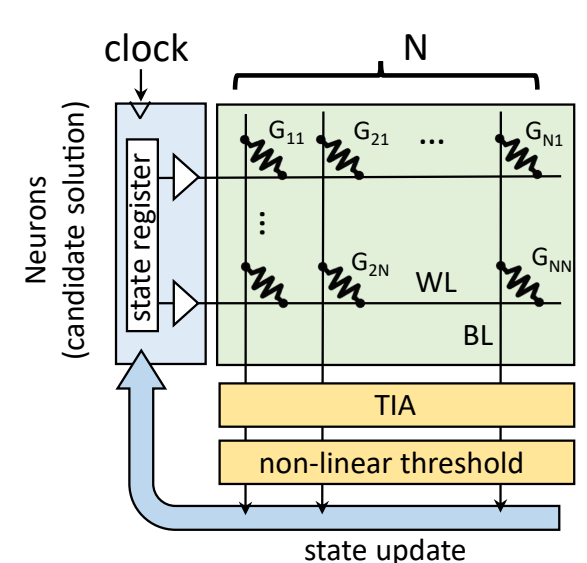
\includegraphics[width=0.3\linewidth]{graphics/Mem_HNN_Modell.png}
    \caption{Modell of the mem-HNN}
\end{figure}
The green square symbolizes the memristor crossbar array, which has the task of performing the in-memory-vector matrix multiplication. 
This is the core part of the architecture that is built around the update formula of the Hopfield Network. 
The memristor crossbar array gets his name because it consists of \textbf{memristors} that connect orthogonal \textbf{electric tracks} with each other.
The \( G_{ij} \) stands for conductance and represents the inverse of the resistance \( R \) of the memristors since \( G = \frac{1}{R}\). On the other hand, \( BL \) (Bitline) and \( WL \) (Wordline) represent the electical tracks.
All the other parts of the model are handled in subchapter 2.4.3, so for now the spotlight belongs to the memristor crossbar array (green square).
A better perspective of the memristor crossbar array gives following 3D model\footcite[cf.][410]{caiPowerefficientCombinatorialOptimization2020}:
\begin{figure}[H]
    \centering
    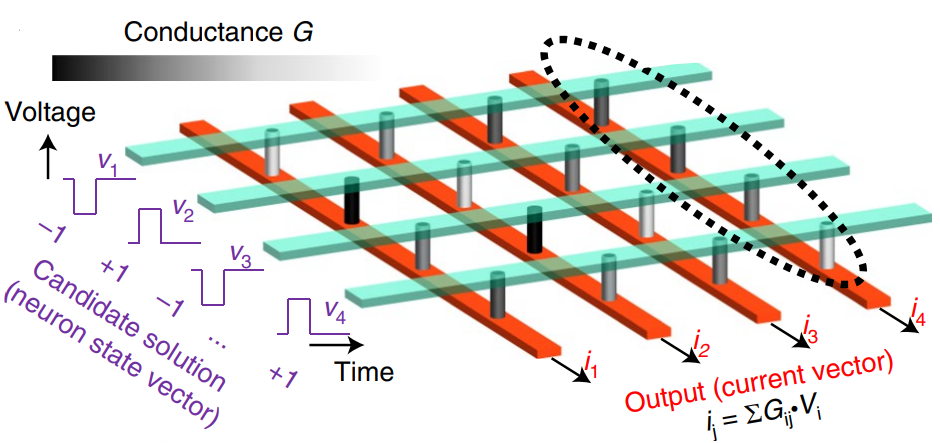
\includegraphics[width=0.65\linewidth]{graphics/memristor_crossbar_array.png}
    \caption{3D modell of the memristor crossbar array}
\end{figure}
To understand how this crossbar array implements the Hopfield network, it helps to have another look at the earlier introduced update formula.
\[
s_i \leftarrow 
\begin{cases} 
+1 & \text{if } \sum_j w_{ij} s_j + b \geq \theta_i, \\
-1 & \text{otherwise}.
\end{cases}
\]
First of all, on the green Wordline a voltage which either is \( +1 \) or \( -1 \) that represent the state of the neurons in the hopfield network is applied.
Then, the current is flowing towards the memristors, which is an electronic device that functions as a resistor, but with the ability to dynamically change its resistance while the device is being used.\footcite[cf][124]{sungPerspectiveReviewMemristive2018}
In this model the gray cylinders represent the memristors.
The memristors are suitable for matrix vector multiplication because they can use their dynamical resistance to act as weigths.\footcite[cf][124]{sungPerspectiveReviewMemristive2018}
In addition to that, this is the reason why this kind of memory has the potential of high switching speeds, high energy efficiency and high endurance.\footcite[cf.][3]{amirsoleimaniInMemoryVectorMatrixMultiplication2020}

In eletrical terminology, if the resistence of a memristor is higher, the conductance is low since the current can barely flow into the lower Bitlane.
For each of the intersections, when a Wordline meets the crossbar it represents the multiplication of \(w_{ij}\) and \(s_j\) within the update formula.
After the matrix vector multiplication the single currents flow in the same direction on the Bitline and are summed up together with their individual current strength.\footcite[cf.][3]{amirsoleimaniInMemoryVectorMatrixMultiplication2020}
The reason for this phenomenon is the 1. Kirchhoff'sche rule, which is not further explained here since it would be out of scope.
To make an example for each output current \(i_{1}\) has for intput voltages \(V_{1}, V_{2}, V_{3}, V_{4}\).
The current flowing into the lower Bitlane is now according to Ohm's rule \( i_{out} = \frac{1}{R_{memristor}} * V_{in}\).
Since \( G = \frac{1}{R}\) and Kirchhoff'sche rule sums up each current \(i\) is \( i_{1} = G_{11}*V_1 + G_{12}*V_2 + \cdots + G_{14}*V_4\)
As a result the first first part \(\sum_j w_{ij} s_j\) of the updating formula of the Hopfield Network is established.
Last but not least, adding the bias \(b\) to the sum is achieved by simply adding an intial current, which is worth the amount of the bias, to the the total Bitline current.
Each i is the output of the current vector and equal to a neuron within the Hopfield Network with all the memristors on this lane symbolizing the weights that all the other neurons connect to it.

Presently, the research on the application of memristor crossbar arrays in supervised learning is sparse, indicating a clear necessity for further investigative studies to understand their potential and usability.\footnote{cf.\cite{amirsoleimaniInMemoryVectorMatrixMultiplication2020}, p. 8; cf.\cite{sungPerspectiveReviewMemristive2018}, p. 124}
In the practical part the \ac{mem-HNN} model exactly this is put to the test and training data of the \ac{RBM} should be generated to give clearance about the feasibility of this idea.


Memristor-based learning
\begin{figure}[H]
    \centering
    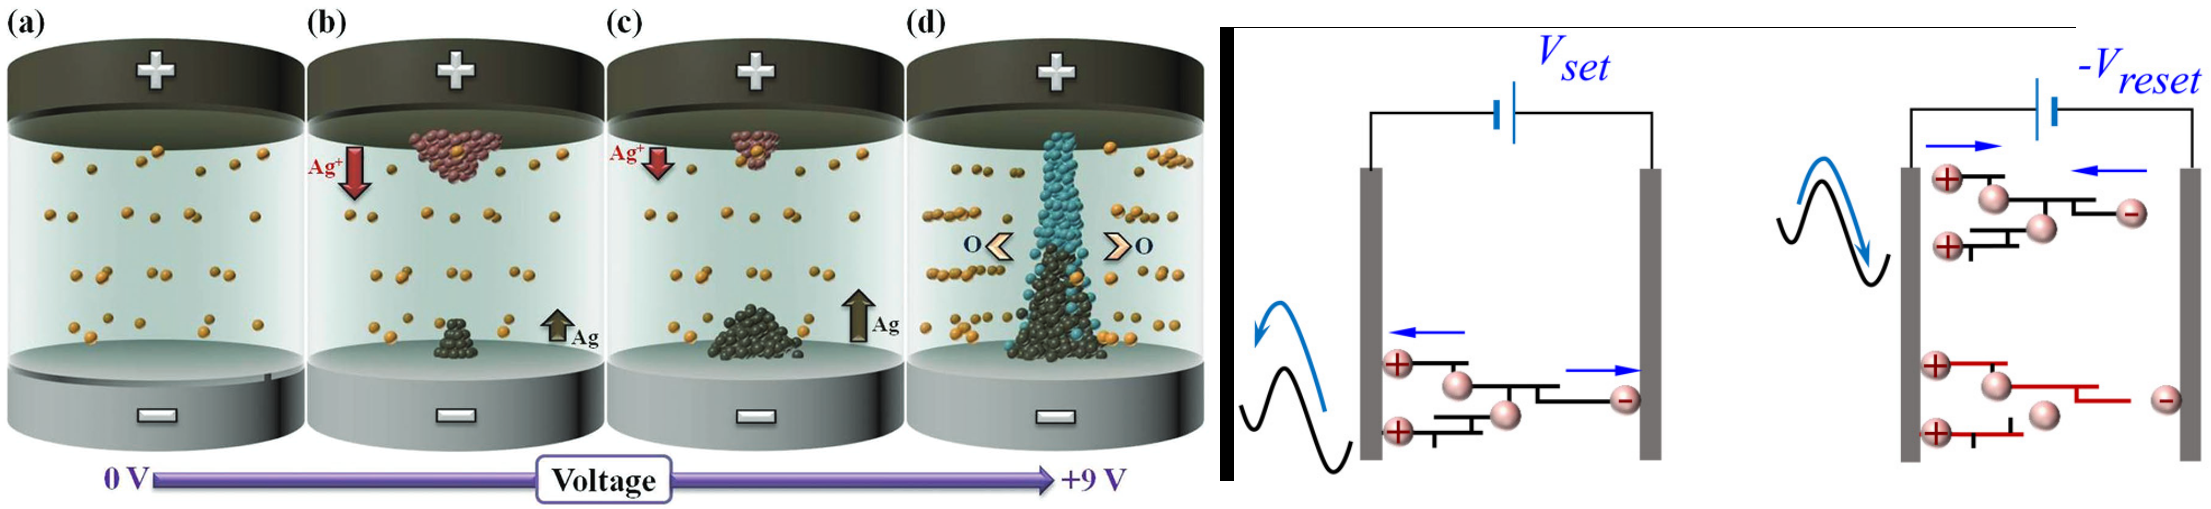
\includegraphics[width=0.8\linewidth]{graphics/Memristor_filoments.png}
    \caption{Memristor-based learning}
\end{figure}


Eher Synapsen interessant
-Wie programmiere ich den elektrischen Widerstand - dieses Konzept kurz erläutern
-Filoment Iformation, wie Plattenkondensator, Wasserleitung mit Ventil, dass man einstellen kann wie viel Wasser durchfließt
- Wie kann man schaffen, dass dieser Widerstand geändert wird?
- Bei hoher Spannung -V reset -> Wenn Hoch genug kann man anfangen Memristor zu verändern 
- 2 Operationsmodi, Programmierphase ermöglicht Wiederstandseinstellen, adere Phase -> Gewichtsmatrix, Strom durchschickeen, also 
geringe Spannung Inferenz. 
-Filament sind Ionen, geladen Teilchen die Srom leiten, bilden gemeinsam Filament (Equivalent wie ein Faden) 
-Spannung wird beim V reset umgedreht, dadurch bricht Verbindung ab. Keine Verbindung mehr da, denn Spannung umgedreht. 
Filament kann auch größer und kleiner werden (Mehr Ionen zusammen), Mehrere Verbindungen möglich,
-Lege Spannng für bestimmte Zeit an und dann lege ich eine Spannung ab und Filament ist gebildet
-Non volatile Memory - im Betrieb, permamenter Speicher, Trainingsschritt trainieren mit V Set, dann -v Reset und V Set für neue Trainingsiteration mit neuen Gewichten
Memristor ist ein nicht volatiler Speicher

---

Kleine Graue Widerstände sind Memristoren,
Das gannze ist das Crossbar Array

Alles zusammen ist das Memristor Hopfield Neural Network


\subsection{Output Hopfield Network}
Alle anderen Bauteile 

TIA, kein Multiplexer mehr = Strom in Spannung umwandeln 

non-linear threshold = Komperator, ist es größer oder kleiner gleich 

Erklärung der Restlichen Bauteile außerhalb des Crossbar arrays (Alles noch Analog)

Hysteretic threshold ist gleich Komperator 

Input/output buffer and driver = State register -> , Buffer = SPeicher und Driver = Sitzt am Anfang des Crossbar arrays als Verstärker 

---

Zusätzlicher Strom auf leiterbahn ist equivalent zum Bias. 

Größer gleich ist mit dem Komperator initialisiert. 

Anfangen mit der Update Funktion -> Dadurch wird Energiefunktion auch implementiert, mit jedem Update wird Energie gesenkt.
Ising Modell ist ne Energiefunktion. Update funktion sorgt dafür, dass lokale minimas der Energiefunktion gefunden werden. 
Für Optimierungsprobleme ist die Lösung dadurch gut genug. 

Ich benutze Sampling mit Rauschen, sodass ich auch mehere Minimas erkennen kann. Wir sind an mehreren Minimas interesiert. 
System starten, iterativ herunterlaufen, in nächstes Minima springen durch rauschen, dadurch Sampling möglcih 

Gewichte werden digital geupdated und ein Eingangssignal mitgegeben 

---


\subsection{Noisy HNN}

Zwischen Bitline(BL) und TIA wird zusätzlich das rauschen noch eingefügt. 


Picture is out of following paper.\footcite[cf.][3]{gmComprehensiveSurveyAnalysis2020}
\begin{figure}[H]
    \centering
    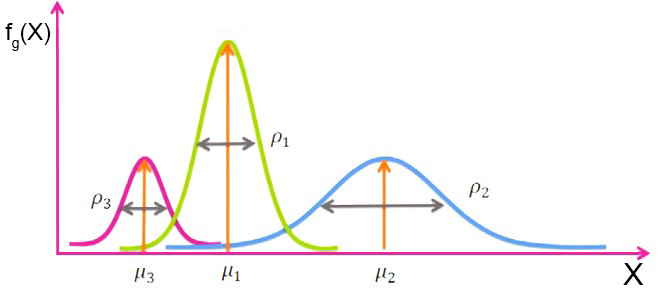
\includegraphics[width=0.7\linewidth]{graphics/Gaussian_Normal_Distribution_edited.jpg}
    \caption{figure of a general Boltzmann Machine}
    \label{fig2}
\end{figure}

\chapter{Objective specification and presentation of the research methodology}

Having laid the groundwork with essential concepts necessary for this thesis,
this chapter aims to outline the objectives of the practical segment as well as the research methodology employed to achieve them.
In the first part, the specific objectives are defined. 
Afterward, in the second part the used research framework \ac{DSR} and the two research methods Prototyping and Simulation are explained.

\section{Objective specification}
The objective of this thesis is to develop a Simulator Pipeline that facilitates the exploration of both the implementation and performance of \ac{BM}s on a \ac{mem-HNN}.
In the beginning, the \ac{IT}-artifact to be implemented is modeled and all components, transitions and processes of the overall solution are identified.
This tool is then used to obtain comparable values in terms of energy consumption and computing speed for a typical workload, relative to Metropolis-Hastings.
Previous research has already shown that Ising machines and \ac{mem-HNN}s are capable of implementing \ac{BM}s.
However, these were proof-of-concepts as mentioned in 2.4.4, where no complete accelerator system was used.
Therefore, no clear statements were possible regarding the actual speed and energy consumption of an accelerator that would allow a comparison with digital computers.
Hence, to answer the primary research questions of this thesis, an \ac{IT}-artifact in the form of a Simulator Pipeline is implemented.
This artifact allows to study of training and inference of \ac{BM}s, where the statistical sampling of activation probabilities is performed with a hardware simulator of the \ac{mem-HNN}.
This hardware simulation contains a behavioral model of the different hardware components of a \ac{mem-HNN} described in 2.4.
To provide insights, key performance metrics for the simulation are identified in the literature: throughput (samples/second) and energy consumption (energy/operation).\footnote{cf.\cite{caiPowerefficientCombinatorialOptimization2020}, p. 409-418; cf.\cite{ortega-zamoranoFPGAHardwareAcceleration2016}, p. 16-17; cf.\cite{aaditAcceleratingAdaptiveParallel2023}, p. 2; cf.\cite{bellettiJanusFPGABasedSystem2009}, p. 55}

Moreover, to allow an intrinsic verification and comparison against conventional sampling methods, the software artifact also includes Gibbs Sampling and Metropolis-Hastings sampling methods.
With the software artifact, an exemplary machine learning workload is analyzed and simulated performance metrics are derived.
This analysis includes the optimization of the \ac{mem-HNN}s hyperparameters as well the different update methods discussed in 2.4.
Then, the performance metrics are intrinsically compared against conventional sampling methods to understand the potential of \ac{mem-HNN}s for sampling and machine learning applications.
By benchmarking these aspects against the conventional methods, this thesis aims to underscore the potential of the \ac{mem-HNN} in practical training of \ac{RBM}s.
Building upon the foundational work, this research also explores the implementation of the N/2 synchronous update mechanism, which anticipates higher sampling speeds and efficiency.

\ac{DSR} is used as a research framework to iteratively create and employ the \ac{IT}-artifact to answer the thesis's research question. 
During the different design iterations, the software artifact is developed using rapid prototyping for the implementation of the \ac{RBM} on the simulated \ac{mem-HNN}.
The last iteration uses a simulation as a research method because the behavior and performance of the system are measured and the underlying model is already finished with the last prototyping iteration. 
Since the practical functionality still requires validation, the \ac{DSR} process,
combined with prototyping and followed by simulation if successful, introduces flexibility and a problem-oriented structure that are crucial for this new method.

\section{Design Science Research}

\ac{DSR} is a core research method within the field of business informatics that ``creates and evaluates \ac{IT}-artifacts intended to solve identified organizational problems''.\footcite[77]{hevnerDesignScienceInformation2004a}
A systematic \ac{DSR} process established by Henver et al. lays a solid groundwork for conducting the research with rigor, offering a degree of confidence that the endeavor will yield meaningful outcomes.\footnote{cf.\cite{baskervilleDesignScienceResearch2018}, p. 368; cf.\cite{hevnerDesignScienceInformation2004a}, p. 77}
Artifacts in \ac{DSR} can be constructs, models, methods or instantiations.\footcite[77]{hevnerDesignScienceInformation2004a}
In addition to that, Gregor and Hevner (2013) categorize the underlying \ac{IT}-artifact based on their abstraction level and maturities.
Hence, level 1 represents a specific, limited and less mature implementation of an artifact, level 2 is operational principles or architecture like constructs, methods or models, while level 3 represents a well-developed midrange design theory.\footcite[cf.][342]{gregorPositioningPresentingDesign2013}
The development of the artifact is performed incrementally with specific goals for each iteration, which is beneficial for \ac{IT}-artifacts that can be adjusted after every iteration.\footcite[cf.][343]{gregorPositioningPresentingDesign2013}

Henver et al. also introduced 7 guidelines that still today serve as a framework for different \ac{DSR} approaches.
Arguably, the most important two guidelines are, that the research must create a viable artifact that in the next step is able to solve the organizational problem. 
Another important guideline is that the artifact needs to be rigorously evaluated in utility, quality and efficiency.\footcite[83]{hevnerDesignScienceInformation2004a}
Thereupon Peffer et al. introduced a well-known \ac{DSR} Process Model, which has 6 different phases: Identify problem \& Motivate, Define Objectives of a solution, 
Design \& Development, Demonstration, Evaluation and Communication.\footcite[cf.][54]{peffersDesignScienceResearch2007a}
Another interesting approach by Österle et. al is called design-oriented business informatics. 
This \ac{DSR} method is used in this thesis for the following reasons.
His approach compresses the phases of Peffer et al. into a more compact model and also gives a more detailed explanation of each phase while still complying with the guidelines established by Henver et al..\footcite[cf.][1-6]{oesterleMemorandumZurGestaltungsorientierten2010}
On top of this promising framework, they created a \ac{DSR} model called consortial research.
It addresses problems for collaborative research in terms of access to practical knowledge, rapid change and practical orientation and a lack of support for knowledge transfer.\footcite[cf.][273-274]{oesterleKonsortialforschung2010}
Österle et al. aims to bridge the gap between the knowledge base of both science and practice, with a focus on evaluating and ensuring the reproducibility of research outcomes.\footcite[cf.][5]{oesterleMemorandumZurGestaltungsorientierten2010}
However, the individual phases of the research framework can also be implemented on their own and the best features 
of the research framework especially the contents of the phases should be combined with its older framework of design-oriented business informatics.
As shown in figure \ref{DSR_Modell} following model is used:
\begin{figure}[H]
    \centering
    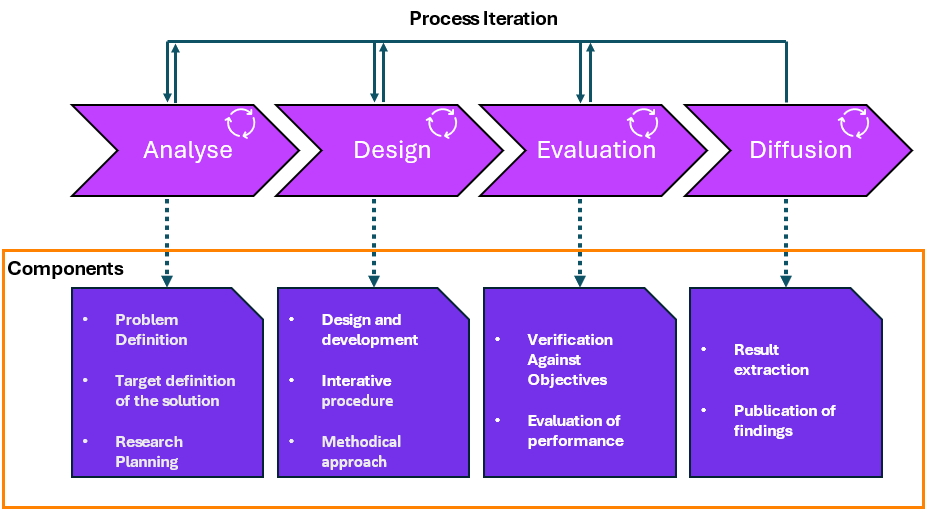
\includegraphics[width=0.9\linewidth]{graphics/DSR_Modell.png}
    \caption{DSR model by Österle et. al\protect\footnotemark}
    \label{DSR_Modell}
\end{figure}
\footnotetext{inspired from \cite[cf.][278]{oesterleKonsortialforschung2010}}
This model uses an iterative process for the phases that allow backward steps to redo an already completed phase if requirements were not satisfied to an appropriate level.
The four phases ideally contain the following contents:

\textbf{Analysis:} This phase identifies and describes the motivation in practice and formulates the desired research objectives.
In addition to that, a vague research plan is introduced which can hold the goals of the project but also underlying constraints. 
Components of the research plan could be external stakeholders, funding, a timetable and of course a concept of the solution.
If possible also a research method should be selected.\footcite[cf.][4]{oesterleMemorandumZurGestaltungsorientierten2010}

\textbf{Design:} The \ac{IT}-artifact is designed and developed with regard to the selected research methodology. 
Specific processes must be justified and comprehensible with consideration of the outcomes of the analysis phase.
The Design process can take multiple iterations on its own with the chance of making adjustments until the requirements are fulfilled.
The outcomes is a functional \ac{IT}-artifact that fulfills the set goals.\footcite[cf.][279]{oesterleKonsortialforschung2010}

\textbf{Evaluation:} Here the established \ac{IT}-artifact needs to be validated against the earlier specified goals. 
Furthermore, it can be validated against the chosen research method. 
This means they must be applicable and they must provide the expected benefit.
If the artifact can not be tested with, for example, a pilot application, it is possible to pursue expert interviews to validate the outcome.\footcite[cf.][279]{oesterleKonsortialforschung2010}

\textbf{Diffusion:} In this phase the results are generally made available to the public.
Therefore, the results need to be prepared for publication in individual communities.
Methods for publication could be teaching at universities and colleges and through their publication in books and specialist journals.
Diffusion in practice also includes the implementation in companies and public administration which the solution was initially developed for.\footcite[cf.][5]{oesterleMemorandumZurGestaltungsorientierten2010}

\section{Prototyping}

Given that the aim of the implementation is to create a new \ac{IT}-artifact with a focus on rapid development, prototyping has been selected as the methodology.
Generally, prototyping is a fundamental practice in designing tools, applications or user interfaces and defining requirements within the framework of agile software development.
It belongs to the agile requirements engineering practice and allows to gather feedback on requirements in a light-weight fashion.\footcite[cf.][1]{bjarnasonModelSoftwarePrototyping2021a}
Prototypes are created to assist in the analysis and design of proposed systems.
A prototype can be defined as ``a simplified model of a proposed system, that is built for a specific purpose'', which can apply to various kind of systems like software, hardware or even people.\footcite[][470]{luqiRapidSoftwarePrototyping1992}
It can be seen as an early increment, model, or release that implements some features of the desired product or model and therefore represents it. 

At the core of prototyping, it comes down to the exploration of the solution space through experimenting with ideas,
collecting feedback and
communicating product requirements in an iterative detailing process.
Hence, prototyping can deliver new requirements that are elicited through exploration and can later be validated 
by testing technical feasibility or business viability.\footcite[cf.][8]{bjarnasonModelSoftwarePrototyping2021a}
A few benefits of prototyping are early construction with low development costs and no large upfront investments of either time or money.
In addition to that, it can promote innovation due to early results that can be communicated and if viable researched further.\footcite[cf.][25]{nelsonSoftwarePrototyping2016}
The reason to choose prototyping can have various reasons. 
This thesis uses this method for the design phase within \ac{DSR} due to the just-named benefits and the possibility of fast results and testing feasibility of the model.

Specifically, G. Arthur Mihram's prototyping model is chosen because it suits well the \ac{DSR} framework and overlaps with it. 
There are five steps to Mihram's prototyping process.
The first step, setting the ``modelling goals'' is already completed with the analysis phase of the \ac{DSR}.\footcite[cf.][71]{mihramSimulationMethodology1976}
Within each iteration in the design phase, a subselection of the goals is chosen to be prototyped. 
Furthermore, the previously established prototype is used as the basis for the following iteration phase allowing to implement more and more features.
In a second step ``systemic analysis'', the prototype can be categorized to set the prototypes behavioural mechanisms.\footcite[cf.][71-72]{mihramSimulationMethodology1976}
As a guideline to categorize this behaviour, the thesis uses the House of Prototyping Guidelines by Ahmed and Demirel.
These guidelines shown in \ref{attachement:prototyping_dimensions} introduce five different dimensions used to categorize prototypes:
Type of Prototype(1), Fidelity Level(2), Complexity(3), Scale(4) and Number of Iterations(5).\footcite[cf.][6-7]{ahmedPrototypingFrameworkHumanCentered2021}

The third step ``model synthesis'' requires a description and a chronological sequences of the prcoesses.\footcite[cf.][71-72]{mihramSimulationMethodology1976}
Furthermore, this is the phase of exploration and ends when the complete set of entities and the environment have been developed in a computer-directed language and the data is provided in machine-readable formats.\footcite[cf.][75-76]{mihramSimulationMethodology1976}

The last steps of Mihram's model: ``model confirmation'' and ``scientific interference'' are not considered since they overlap with the \ac{DSR} phases of evaluation and diffusion. 
This simply prevents a duplication of work.
Therefore, the categorization of the prototype and afterwards the ``model synthesis'' is executed per iteration in the prototyping model used in this thesis. 

\section{Simulation}

Simulation has been chosen as the methodology for the evaluation phase of the \ac{DSR} framework to collect data.
This is necessary because the \ac{mem-HNN} is still under development and actual devices with the functionality required for the implementation for \ac{BM}s are not yet available.
In these development phases of hardware devices, it is therefore common to use simulation tools, that allow fast and accurate predictions of performance long before actual measurements on a device are possible.
A simulation model can be defined as a computerized representation of a given model capturing its dynamic behavior.
The primary motivation for establishing a simulation model or using any other modeling method like prototyping is that it is
a cheap and fast way to gain important insights without being exposed to the following constraints: costs, risks or logistics of manipulating the real system.\footcite[cf.][92]{kellnerSoftwareProcessSimulation1999}
A single \ac{ASIC} chip has a long development time due to the complex layout and fabrication process and can cost between 10.000 to 100.000 USD.
Furthermore, the gathered data helps with decision-making at strategic and operational levels.\footcite[cf.][93]{kellnerSoftwareProcessSimulation1999}
For example, with the results of a simulation, it can be decided if the new hardware works like expected and can be set up for production.
These are the reasons why the simulation methodology is chosen for the evaluation phase of the prototype. 

Computer simulation involves adjusting a computer-based model to better analyze how a system behaves and to evaluate approaches for their operation, either for descriptive or predictive purposes.\footcite[cf.][13-14]{abarAgentBasedModelling2017}
In the case of the \ac{mem-HNN}, there is a need for the evaluation of software performance in combination with the hardware to gather proper data.
The reason for this is that only using a functional software simulation without considering the hardware specifications results in a decreased price and time but with a significant precision loss.\footcite[cf.][470-471]{sarhadiStateArtHardware2015}
However, precision and efficiency are a key part of being able to answer the research question.

A general simulation model published by Kellner/Madachy/Raffo can be seen as an overview of the work in the simulation field.
It consists of the following entities: (0) model purpose, (1) model scope, (2) result variables, (3) process abstraction and (4) input parameters.  

\begin{figure}[H]
    \centering
    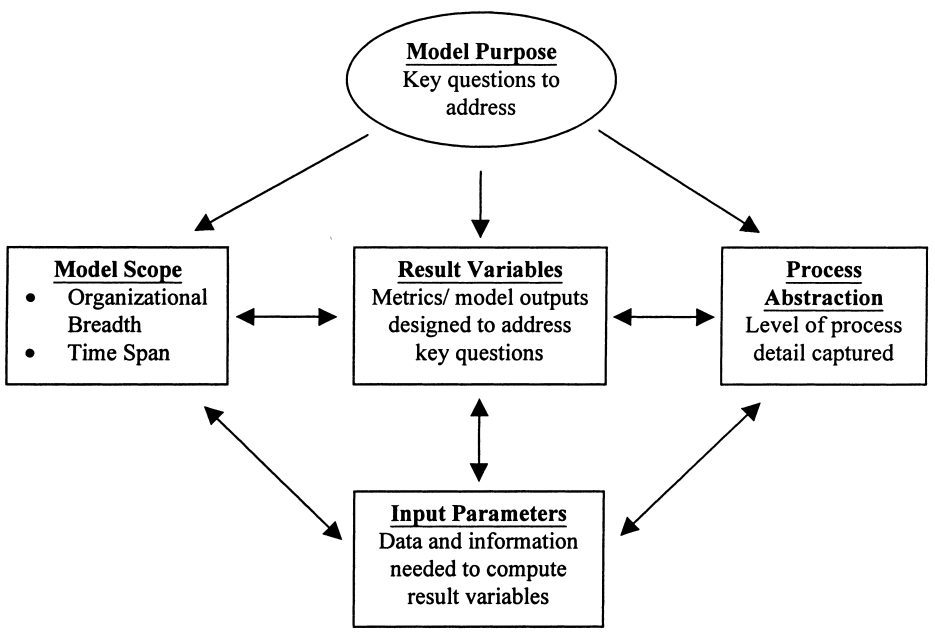
\includegraphics[width=0.7\linewidth]{graphics/Simulation_Modell.png}
    \caption{general simulation model\protect\footnotemark}
    \label{simulation_Modell}
\end{figure}
\footnotetext{\cite[][95]{kellnerSoftwareProcessSimulation1999}}

The general \textbf{model purpose} is based on the specific research question that needs to be answered.
It is crucial to thoroughly understand the effects based on this key question to ensure the correct selection of the \textbf{model scope}.\footcite[cf.][95]{kellnerSoftwareProcessSimulation1999}
This can be an iterative process that includes the selection of a scope, for example, a development project, long-term product evolution etc. and within 
this scope, an estimated timespan (short(less than 12 months), medium (12-24 months), long (more than 24 months)) needs to be selected. 
In addition to that, the organizational simulation width is set (less than one project team, one project team, multiple project teams).\footcite[cf.][96]{kellnerSoftwareProcessSimulation1999}

The \textbf{result variables} are information elements that are the central key entity of the simulation model. 
They change based on the main question being asked, representing the crucial signs of a successful simulation.
Typical metrics for software simulation could be: effort/cost, throughput/productivity, queue lengths in the backlog,
energy efficiency, return on investment.
Furthermore, with one simulation multiple result variables can be gathered simultanously.\footcite[cf.][96-97]{kellnerSoftwareProcessSimulation1999}

\textbf{Process abstraction} includes the inner structure of the simulation model.
Therefore, all the processes, vital resources, dependencies and iteration loops need to be considered to achieve the desired result variables and to answer the key quesions.\footcite[cf.][97]{kellnerSoftwareProcessSimulation1999}
Lastly, the \textbf{input parameters} consider all the parameters that are needed to produce viable outcomes. 
This can range up to hundreds of data parameters to achieve the desired results. 
In theory, these parameters can also be extended to human resources like software engineers who are needed for their skills in programming knowledge.\footcite[cf.][97-98]{kellnerSoftwareProcessSimulation1999}

This general usable simulation model is not only part of the \ac{DSR} evaluation phase but also part of the \ac{ASIC} design process. 
Therefore, the model is modified to match the needs for a performance simulation of the \ac{mem-HNN}.
The simulation model is part of the architecture and high-level design of the \ac{ASIC} design process.
It involves selecting key components like processors, memory blocks, and communication interfaces and carrying out a functional verification through a suitable simulation.\footnote{cf.\cite{raoUltimateGuideASIC}, p. 1; cf.\cite{ASICDesignFlow}, p. 1}
The modification to the model is expressed through the actual energy model of the \ac{mem-HNN}, which is added to the simulation model, that can compute energy usage per clock cycle. 
Hence, depending on a specific input it can calculate how much energy was required to do computations that are the output and used for the next cycle. 

\chapter{Implementation of the mem-HNN}

\section{Objectives and research methodology}
Upon establishing the precise research methodology, this chapter delves into the implementaiton of the simualtor pipeline.
First, the analysis phase of the \ac{DSR} process is executed with the goal to establish a model of the simulator pipeline,
which the requirements and conditions can be derived from. 
Next, a practical prototype is developed in iterative design cycles to fulfill the target requirements.
In the evaluation phase, the simulator pipeline is used to assess the performance of the \ac{mem-HNN} 
in the training of an examplary machine learning workload. 
This thesis utilizes performance metrics collected from the simulation to address the central research question, which explores potential speed and efficiency enhancements of the \ac{mem-HNN} compared to digital computers.


\section{Analysis phase}
\subsection{General conditions}

Following the first phase of the \ac{DSR}-cycle described in Chapter 3, the research outline is initially established from which the requirements for the simulator pipeline are derived.\footcite[cf.][278-279]{oesterleKonsortialforschung2010}
This analysis begins by describing the general conditions specified in Section 3.1.
Hereby, general conditions are permanent design decisions that are used as foundation for the implementation of the simulator pipleine.
The underlying motivation hereby is to research if the known proof of concepts are feasible on the complete \ac{mem-HNN}
and evaluate if that brings an actual acceleration, which is equivalent to answering the research question of this thesis. 

The implementaton is executed in the programming language Python since it offers a variety of third party libraries that are useful 
for machine learning that are state of the art, like pytorch, scikit learn etc..\footcite[cf.][306-307]{DiscreteContinuousModels}
Furthermore, Scikit Learn is chosen as machine learning library since it is one of the industry standards for classical machine learning, has a broad variety of features in terms of \ac{BM}s
and has a lower learning curve compared with e.g. Tensorflow.\footcite[cf.][5-6]{raschkaMachineLearningPython2020}
For simplicity and to save time, an \ac{RBM} is used as a test case with handwritten digit classification as workload.

The complete \ac{mem-HNN} is beeing simulated based on a design that has been developed by the Forschungszentrum Jülich and HPE.\footcite[cf.][3-4]{hizzaniMemristorbasedHardwareAlgorithms2023}  
This design describes an \ac{ASIC} design that realizes the noisy Hopfield Network shown in figure\ref{ModellHMM}.
It includes an energy model based on low-level circuit-simulations, which can derive the average energy consumption per clock cycle of the \ac{mem-HNN}.
In addition to that, the model includes latency estimations of the \ac{mem-HNN} to perform a full iteration. 
This simualtion approach is chosen as the device is still under development and hardware devices are not available yet.
Nonetheless, the complete hardware can be realized in software without compromising its functionality.
Such a simulation based performance evaluation is quite common in the \ac{ASIC} design flow.\footnote{cf.\cite{raoUltimateGuideASIC}, p. 1; cf.\cite{ASICDesignFlow}, p. 1}
A in-depth explanation of this model is out of scope for this thesis but core parameters are explained to understand the gathered energy values.
Lastly, the simulation is performed on a notebook.
Due to the limitations of the built in \ac{CPU}\footnote{\texttt{Intel i7-10610U, 1.80GHz, 2304 MHz, 4 Cores, 8 Logical Processors}}, efficient coding is required to ensure simulations are performed within an acceptable timeframe.

\subsection{Requirements}

To evaluate the performance of \ac{mem-HNN}s in training and inference of \ac{BM}s, a full simulator pipeline has to be modeled.
In Fig.\ref{Overall architecture} the envisioned model is shown, in which an \ac{mem-HNN} chip can be used to implement \ac{BM}s.
Here, a digital computer is used to implement and train machine learning models on vairous datasets.
The \ac{mem-HNN} chip is then used to perform the sampling during the \ac{BM} inference or training.
Training and inference on this system then involves the following five steps, which are handled by different components and desribe the iteraction between the digital computer and the analog \ac{mem-HNN} chip:
\begin{figure}[H]
    \centering
    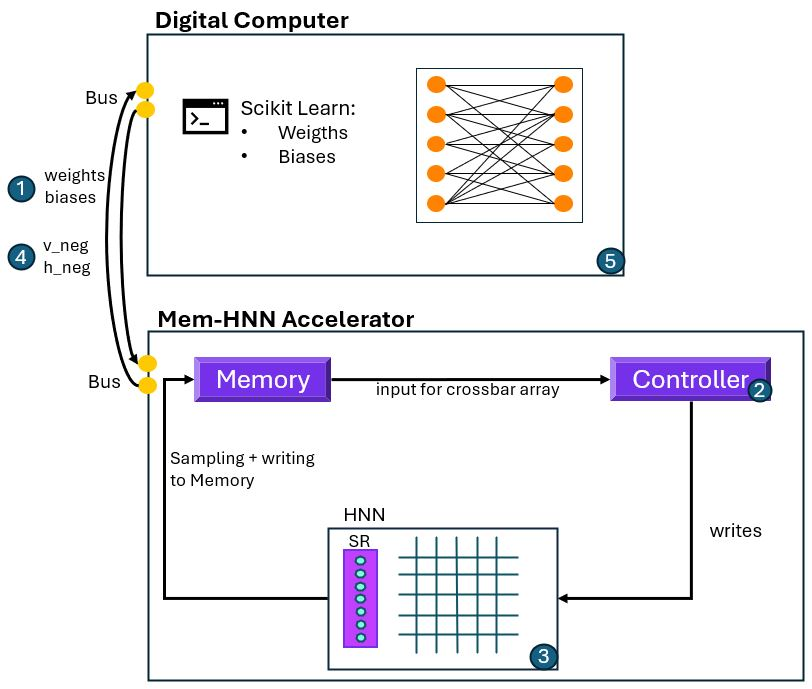
\includegraphics[width=0.80\linewidth]{graphics/Analysemodell.JPG}
    \caption{proposed solution architecture}
    \label{Overall architecture}
\end{figure}
\textbf{1.} initializes the machine larning model (neural network) including setting the weights and biases of the \ac{BM}. 

\textbf{2.} starts with the transfer of the weigths and biases to the \ac{mem-HNN} accelerator via a bus-system. 
The local memory saves the data and forwards them to the controller. 
The controller is able to programm the memristors in the crossbar array. 

\textbf{3.} is the Hopfield Neural Network (HNN), which contains the memristor crossbar array and the state register (SR).
Here, \ac{mem-HNN} performs a pre-defined amount of iterations, where a sample configuration is stored in the on-chip memory after each iteration.\footcite[cf.][18]{caiHarnessingIntrinsicNoise2019}
The state register includes the current neuron configuration and can lock und unlock specific neurons, so that it is possible to update neurons synchronously.\footcite[cf.][18]{caiHarnessingIntrinsicNoise2019}
This enables the possibility of the promissing N/2 update strategy.

\textbf{4.} After the \ac{mem-HNN} has performed all iterations, the stored sample configurations
of the visible \(v_{neg}\) and the hidden \(h_{neg}\) neurons are transferred back to the digital computer via the bus-system.

\textbf{5.} With the sample configurations, the digital computer calcualtes the activation probabilities and performs
the updates to the weights and biases according to the trainign rule in equation\ref{Update_weights}.
These training updates are repeatley performed starting again from step 2 until the model achieves sufficient performance.
Furthermore, the model can be evaluated in its performance in terms of chosen metrics like prediction accuracy or the negative likelihood etc..

In the simulator pipeline the behavior of the \ac{mem-HNN} in fig.\ref{Overall architecture} is mimicked, where the simulator acts as a drop-in replacement until hardware devices become availbale.
The simulator models the behavior of the chip, so that performance predictions are possible long before a hardware device can eventually be used.
Here, it is important to stress that the current hardware model described in the previous section currently does not contain modeling results for the on-chip memory, the controller and the bus system.
The simualtor is therefore solely focused on modeling the sampling step 3.
With more modeling results becoming available, accurate simualtions of step 2 and 4 can be added to the simualtor.
The next step is to derive the requirements and to establish the research outline.
The aim of generating requirements is to generate good quality, requirements that offers an acceptable level of risk to start the project.\footcite[cf.][11]{ebertSystematischesRequirementsEngineering2008}
These requirements need to cover the functions of the \ac{mem-HNN}, which then must be implemented by the respective software components.
Also, requirements may evolve over time and require adjustments when outcomes differ from initial expectations.
As a result, considering the research question and objectives, the following software requirements emerged:

\textbf{Digital Computer}
\begin{itemize}
    \item Initialize a \ac{BM}
    \item Utilization of any training data
    \item Initializing of other ML models that are used in conjucntion with the \ac{BM} for evaluation
    \item Training of the \ac{BM} with either Gibbs Sampling or Metropolis Hasting
    \item Setting individual parameters: sampling steps, training iterations, noise level, learning rate 
    \item Evaluation of the model's performance using prediction accuracy and negative likelihood
\end{itemize}
\textbf{Simulated Mem-HNN Accelerator}
\begin{itemize}
    \item Using any \ac{BM} as input
    \item Implementing the noisy Hopfield Neural Network update mechanism described in \ref{noisy_update_HNN_formula}
    \item Return sampled output of the neuron configurations 
    \item Selectively switching between the N/2 half updating method instead of single spin updates described in 2.4
    \item Simulation of computation speed (throughput) and energy consumption of the \ac{mem-HNN} chip
\end{itemize}
Furthermore, the python program should be split logically into the different modules and components to enable well structured code. 
With set requirements it is now possible to begin the iterative design and evaluation cycle with focusing on some requirements per iteration.

\section{First Design and Evaluation phase}

This \textbf{Design phase} has the goal of implementing the parts of the simulator pipeline that is executed 
on the digital compuer in fig.\ref{Overall architecture} requirements.
Accordingly the resulting prototyp of this iteration has to satisfy all requirements listed under digital computer in section 4.2.
The implementation is verfied with a test case based on classification of handwritten digits.
The first step in the described prototyping methodology within 3.3 is to perform the systemic analysis to categorize the prototype.
In the realm of prototyping, the following categorizations are made: the prototype type (1) is computational, and its fidelity level (2) is high, as it aims to model all functionalities closely to reality.
Furthermore, the complexity (3) is considered moderate because not all hardware components can be modeled in software.
Additionally, the scale (4) remains constant, and there are multiple iterations (5) executed sequentially to train and infer the \ac{RBM}.
This process of categorizing the protoype helps to make prototypes comporable as prototyping can be used very vague.
The second step, is to set up the Scikit Learn machine learning library as explained in 4.2.
Scikit Learn includes built-in models for \ac{BM}s that enable rapid development also includung popular datasets, delivering results that are comparable with those found in literature.
This is useful to answer the research question in a timely manner.
Especially, the test case used for the \ac{BM} is based on an example of the official scikit learn documentation.\footcite[cf.][1]{RestrictedBoltzmannMachine}

The following task is to set parameters like the learning rate, iterations, size of the hidden layer. 
With having a look in the literature and through testing a learning rate of \(0.2\), 10 training epochs with 72 iterations in one epoch, and an hidden layer of 100 neurons is chosen.\footnote{cf.\cite{hintonPracticalGuideTraining2012}, p. 11-12; cf.\cite{bohmNoiseinjectedAnalogIsing2022}, p. 1}
The size of the visible layer is automatically recognized by Scikit Learn, so for example to 64 to correspond with 8x8 images of a dataset.
Also, the dataset implementation can be customized as needed, such as for a breast cancer classification workload.

The training of the \ac{RBM} is performed in the \texttt{.fit} method and for the functionality to select the preferred sampling algorithm an additional sampling method need to be added.
This process includes modifying the \texttt{\_rbm.py} file in the basic scikit learn library.
The predefined sampling method is gibbs sampling and there is no option to access metropolis hasting within the basic library. 
Therefore, the metropolis hasting alhorithm, explained in 2.2.3 needs to be manually implemented.
The according adjustments are included from the code availability of a paper.\footcite[cf.][11-12]{bohmNoiseinjectedAnalogIsing2022}
This decision is made because the algorithm used there is the original metropolis algorithm by Metropolis et.al..\footcite[cf.][1087-1092]{metropolisEquationStateCalculations1953}
Furthermore, the implementation is performant with many numpy functions. 
To utilize this sampling method, some minor adjustments are made for the user friendliness. 
First, one function is fixed that has a small error, which produced an erroneous empty configuration as the first sampling iteration. 
The user friendliness is achieved by introducing a new parameter \texttt{sampling\_method} that dynamically allows to change the sampling method. 
Another change is the approach of evaluating the performance of the neural network after an x amount of iterations to meassure its performance on the test data while training.
A complete code overview of the metropolis hastings sampling algorithm can be found in the \texttt{mcmc2.py} file as part of the digital delivery with all
adjusted methods for the training of the \ac{RBM} in \texttt{\_rbm.py}, while the overall execution takes place in the \texttt{playground.py}.

To evaluate the results and functionalities the \textbf{Evaluation phase} in this iteration validates the functionalities through a training of the \ac{RBM}. with each sampling method and extract their prediction accuracy.
Scikit learn offers a variety of datasets that are already in a polished format, ready to use. 
The decision is to use a classification workload of handrwritten digits as a test case for validating the implementation.
One reason for this is that the ``load digits dataset'' is similar to the well known MNIST dataset representing an industry standard problem, but has a smaller resolution of 8x8 pixels and features around 1800 samples that can be categorized in 10 classes (integers 0-9).\footcite[cf.][1]{SklearnDatasetsLoad_digits}
The second reason is that the workload is already optimized and therefore can deliver relevant data for the research question.
In this case additionally a nudging of the data is chosen to create more samples, by a factor of five, and to bring more complexity in the workload. 
The split in the dataset is selected to be divided into the conventional 80\% training data and 20\% test data.\footnote{cf.\cite{charithaTypeIIDiabetesPrediction2022a}, p. 1-2; cf.\cite{supriAsianStockIndex2023}, p. 1}
For training, an \ac{RBM} is selected as the feature extractor and paired with a logistic regression classifier for prediction, thereby establishing a cohesive pipeline.
Following figure\ref{CD_baselines} shows the training results using the gibbs sampling approach. 

\begin{figure}[H]
    \centering
    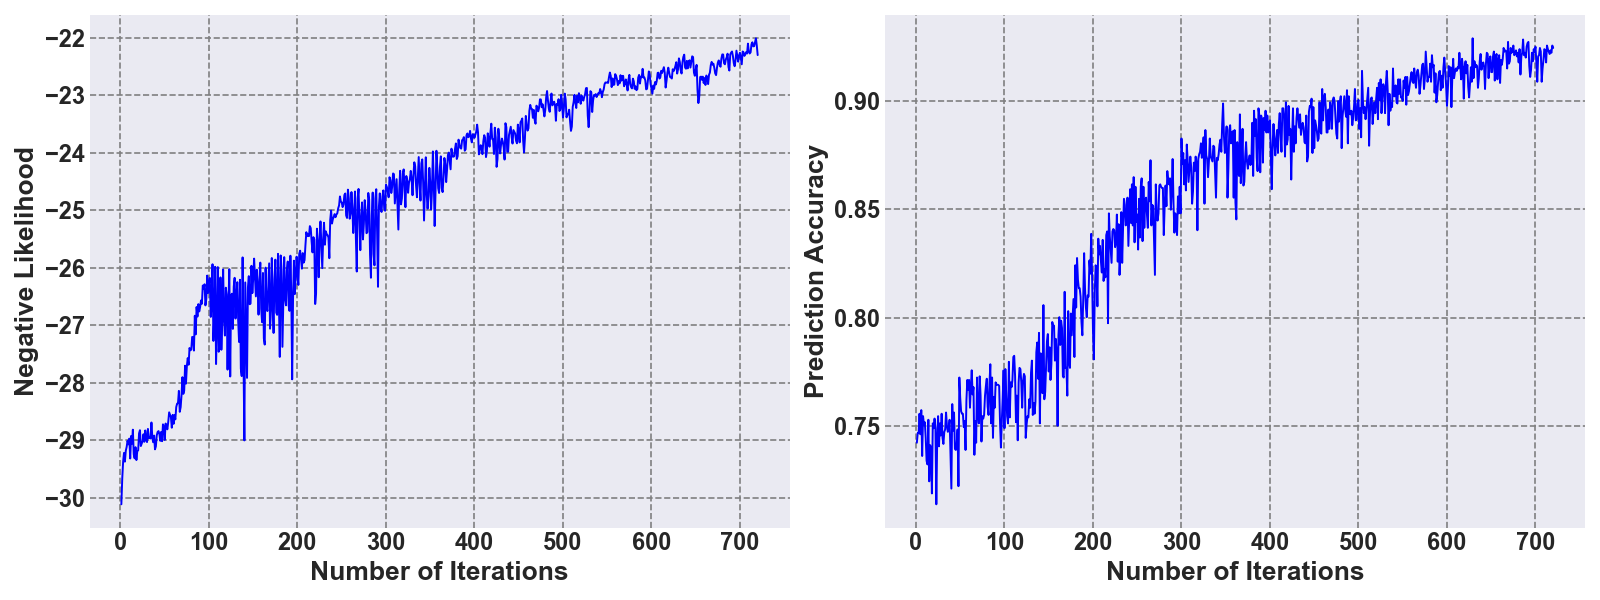
\includegraphics[width=0.9\linewidth]{graphics/CD_combined_plot.png}
    \caption{Gibbs sampling baselines}
    \label{CD_baselines}
\end{figure}
The right plot shows that the initial prediction accuracy starts at 75\%, akin to that of just a single linear regression model.
This suggests that the untrained \ac{RBM} at the input of the classifier initially does not effect the model's classification performance.
Data points are colected after every iteration across the span of 720 iterations. 
After 650 iterations the accuracy slowly stagnates and has a maximum prediction accuracy
of 92.29\%. 
In the left plot picturing the negative likelihood, which is a measure of how well a statistical model represents the observed data.
When training a model the aim is to minimize the negative log-likelihood, which means that the model maximizes the probability of generating the observed data.
Hence, it is visible that in the beginning the model learns more rapidly and in steadily grows its knowledge with some smaller break-ins at the end.
The best value is a negative likelihood of -22.01.
\begin{figure}[H]
    \centering
    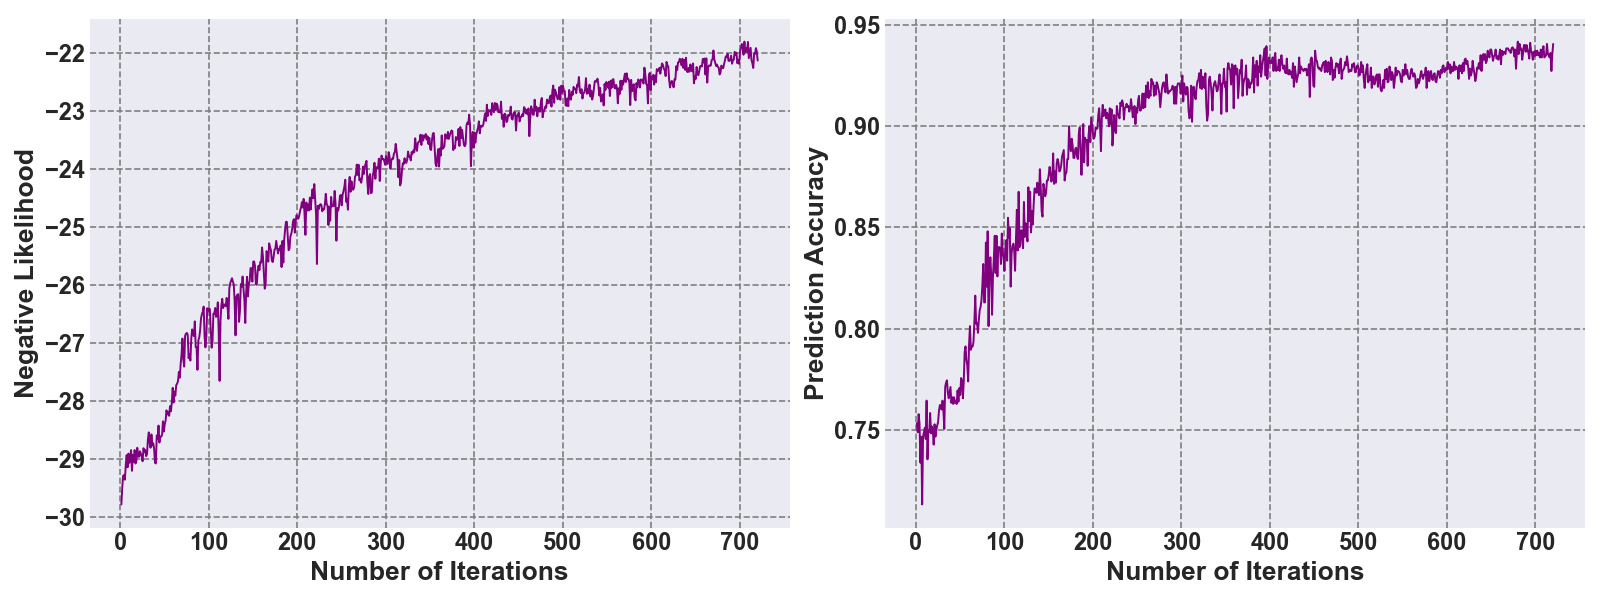
\includegraphics[width=0.9\linewidth]{graphics/metropolis_combined_plot.png}
    \caption{Metropolis sampling baselines}
    \label{metropolis_baselines}
\end{figure}
In contrast, the fig.\ref{metropolis_baselines} used the sampling algorithm of metropolis hasting to train the \ac{RBM}.
Noteworthy is that the prediction accuracy in the right plot has a faster increase in the beginning but already starts to stagnate at around 400 iterations. 
Here, the maximum prediction accuracy achieves 94.15\%. 
The negative likelohood is also growing faster than in Gibbs sampling and exhibits less variablitiy showing a more continuously learning rate.
Here, the best negative likelihood value is -21.80.
Furthermore, to validate the accuracy of the results, they are compared against similar results to those from the literature.\footnote{cf.\cite{bohmNoiseinjectedAnalogIsing2022a}, p. 5; cf.\cite{RestrictedBoltzmannMachine}, p. 1}
Therefore, a good agreement is visible, suggesting that the implementation produces valid results and can thus be considered correct.
As a result, with each sampling method successfully undergoing a training, all the functionalities can be proven right and the prototype can be passed 
into the next design iteration.
The gathered data can later on be used as baseline against the desired new updating mehtod of sampling with a Hopfield Network.


\section{Second Design and Evaluation phase}

This \textbf{design phase} iteration has the goal of implementating the simulator for \ac{mem-HNN} chip shown in fig.\ref{Overall architecture}.
The functionality of this chip is that of a noisy Hopfield Neural Network, which has previously been described in 2.4.4.
The update mechanism is based of he update formula in eq.\ref{noisy_update_HNN_formula}, where noise is injected to imitate the stochastic behaviour of the neurons.
Hence, a \ac{BM} can be modelled by correctly tuning the noise of the Hopfield Neural Network.
Following subfunctionalities need to be established: drawing random neurons to update,
correct injection of the gaussian noise scale, calculating the weighted sum,
comparing the weighted sum + bias + noise against the threshold and saving the new neuron configuration.
Furthermore, the possibility of selectively switching between the N/2 half updating method instead of single spin updates
is to be included in this design phase. 
Hence, this iteration aims to break new ground as it involves implementing the Simulator Pipeline, which has not yet been validated, and integrates the noisy Hopfield Network with the capability for N/2 half updating.

The Hopfield Network is initialized with a size of just one neuron and an sampling iteration counter of \(1500\) iterations with a thermalization of \(100\) sampling steps before 
the neuron is updated.
Thermalization is included to allow the network to perform independent sampling steps and get into a flow to ensure unbiased sampling steps.
The threshold as defined in the update formula is \(0\). 
As experimented the update formula for the implementation of the Hopfield Network looks the following:

\begin{lstlisting}
    for x in range(self.iterations_per_theta):
                    
        self.neuron_index = np.random.randint(0, self.size) #pick a random neuron in the network
        # Calculate the weighted sum for the neuron, excluding its own state
        weighted_sum = sum(self.weights[self.neuron_index][j] * self.configuration[j] for j in range(len(self.configuration)) if j != self.neuron_index)

        self.new_configuration = deepcopy(self.configuration)   #copying the old configuration to create a new one and update it
        if (weighted_sum + self.bias + np.random.normal(0, scale=1.75)) >= self.threshold_theta:          
            self.new_configuration[self.neuron_index] = 1
        else:
            self.new_configuration[self.neuron_index] = 0
            
        self.configuration = deepcopy(self.new_configuration)   #Cloning current configuration and updating the cloned version to the new configuration after comparing with threshold

        if x >= self.thermalization:  
            self.summedConfigurations = self.sum_configurations(self.summedConfigurations, self.new_configuration)    
            self.iterationcounter += 1
        
    self.activationProbabilityPerNeuronDict[self.bias] = self.divide_array_elements(self.summedConfigurations, self.iterationcounter)
    self.bias += 0.025
\end{lstlisting}

The code represented here shows the update meachnism for the single spin update. 
In the beginnig a random neuron is drawn to be updated, which currently everytime is neuron number one because the network size is initialized with one neuron. 
Calculating the weighted sum can be seen as the core of the update formula and is executed first.
Therefore, the weight matrix is selected (indexed by the random drawn neuron) and multiplied by the current configuration resulting in 
the weighted sum that also ignores the weights connected from the drawn neurons.
Afterwards for the comparison against the threshold the according bias of the neuron is added together with the injected noise (scale).
To achieve the injection of noise, a Gaussian normal distribution is added which can modify the activation function, making it compatible with the sigmoid function.\footnote{cf.\cite{bohmNoiseinjectedAnalogIsing2022}, p. 1-2; cf.\cite{mahmoodiVersatileStochasticDot2019}, p. 2}
Technically this is performed by adding \texttt{np.random.normal(0, scale=1.75)} to the weighted sum and the bias, with 0 beeing the mean of the distribuion and the scale representing the standard deviation. 
Hereby, it is important to find a standard deviation that is very close to the true activation probability is important, otherwise the training of the RBM would not work.
In addition to that, the standard deviation changes with neuron size and needs to be readjusted if changes are made to the networks structure.
Next, if the weighted sum plus bias and noise exceeds the threshold, the corresponding neuron state is set to 1; otherwise, it is set to 0.
Lastly, after enough iterations when the thermalization is exceeded the new configurations
are summed up to enable calculating the activation probability of the neurons. 

For the sake of readability the N/2 half update mechaism is seperated but the used selective method with an according parameter is available in attachment \ref{attachement:HNN_N/2Half Code}.
Hence, in a next step the possibility of the N/2 half updating methdod should be implemented as already mentioned in 2.4.3 and 3.1.
N/2 half is updating neurons synchronously instead of the conventional asynchronously (only one neuron is chosen and updated) used in the Hopfield Network updating mechanism.\footcite[cf.][23-24]{caiHarnessingIntrinsicNoise2019}
Following adsjustments are made in the code to achieve this behaviour:
\begin{lstlisting}
    self.neuron_index = np.random.randint(0, 2, self.size) #pick complete random neurons in the network, result [0,1,1,0,...]

                weighted_sum = np.dot(self.weights[:, :], self.configuration)   
                self.new_configuration = deepcopy(self.configuration)
                bias = self.bias 

                for i in range(len(self.neuron_index)):              
                    #updating function comparing against threshold
                    if self.neuron_index[i] > 0:
                        if (weighted_sum[i] + bias[i] + np.random.normal(0, scale=self.scale)) >= self.threshold_theta:          
                            self.new_configuration[i] = 1
                        else:
                            self.new_configuration[i] = 0
\end{lstlisting}
The randomly drawn neuron index now assigns either a 1 or a 0 for each neuron over the size of the network.
Hereby, a 1 means that the sum of this neuron is calculated and will be compared against the threshold. 
As a result, in a completely random process this would lead to about 25\% of all neurons updated (\(50\% drawn * 50\% updated\)).

Coming back to the last two lines of the first code block, the resulting activation function is obtained by summing all configurations within a single bias configuration.
In a next step, the configurations counted are divided by the number of total sampling iterations within the bias configuration (in this case 1500 iterations).

With the resulting file \texttt{\_hopfield\_network\_v1.py} the aim is to \textbf{Evaluate} the establihed noisy Hopfield Network with a single neuron 
and meassure its activation function.
Like mentioned in 2.4.4, a Hopfield Network has a binary activation function that needs to be made compatible with the sigmoid activation function of the \ac{RBM}.
The decision to use a single neuron enables fast iteration times and clear results on how the network behaves, facilitating the measurement of activation probability.
Once the noise injection proves stable and effective for a single neuron, it proves that it will work for coupled neurons.
The value of the bias ranges from \(-6; 6\) in step sizes of \(0.025\). After completing all sampling iterations beginning with \(-6\) the step size is added to the bias until all iterations are made.
This is sufficient to completely cover an ordinary Hopfield Network with its range of the neuron activation function. 
That following figure \ref{Noisy_acitivation_function_bad} visualizes the resulting activation probability of the single neurons. 
\begin{figure}[H]
    \centering
    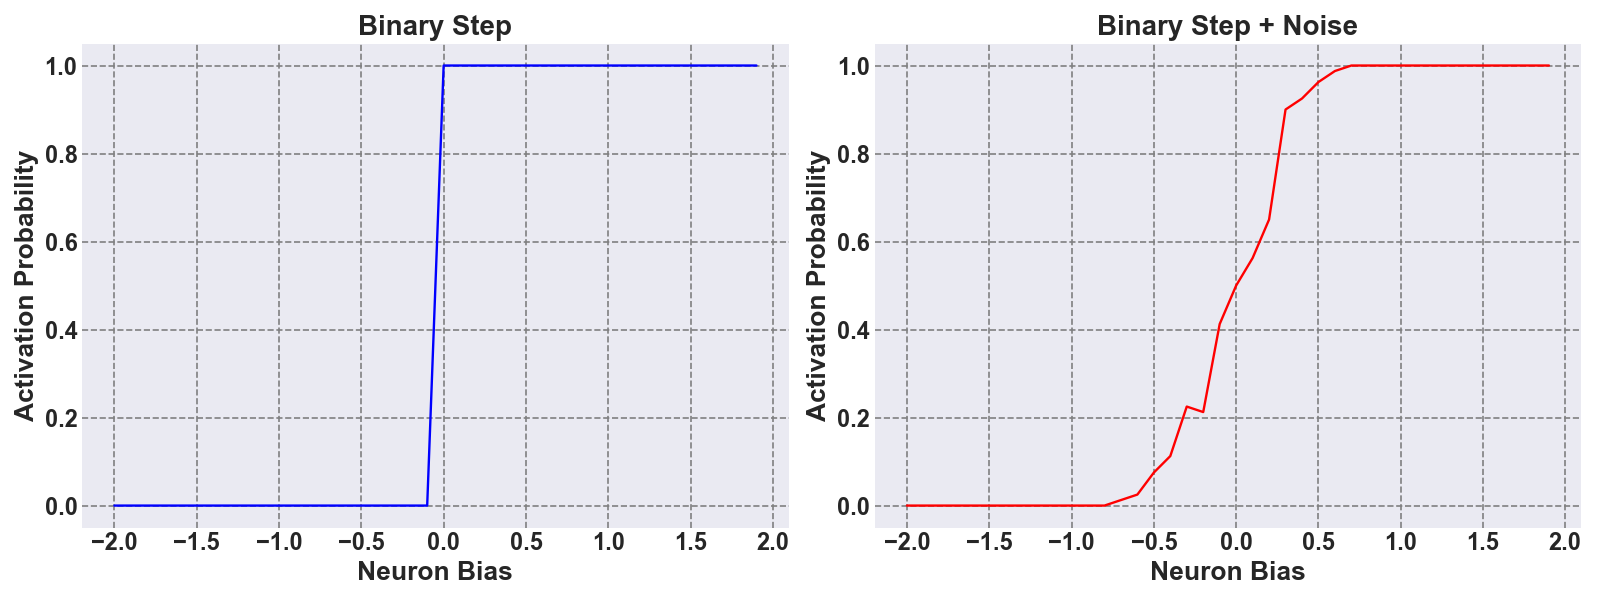
\includegraphics[width=1\linewidth]{graphics/combined_noise_activation_plots.png}
    \caption{Modification of the the Hopfield Network binary step activation function}
    \label{Noisy_acitivation_function_bad}
\end{figure}
In the left plot, visualized in blue, the activation probability of the neuron is shown without adding noise to the plot. 
The behaviour is like one would expect it; once the bias reaches 0 the neuron is activated all the time.
In the right figure with the the red line a noise of \(sigma=0.3\) is added.
The resulting activation is probabilistic and follows a rudimentary sigmoid shape, very similar to the activation function of a \ac{BM} shown in fig.\ref{logistic_sigmoid}.
The right plot shows that the noise injection works, even though it doesn't perfectly copy the sigmoid function.
Concluding from this the sigmoid function is not achieved and the trainig of an \ac{RBM} probably fails. 
Therefore, to completely evaluate and ensure that the injected noise fits to the logistic sigmoid function, the function itself is plotted 
as index, to have a visual comparison. 
Now, finding the correct standard deviation is the goal. 
In following figure\ref{Noisy_acitivation_function_good} the hyperparameter is tuned and the resulting scale is visualized.
It verifys that a noisy activation function of a Hopfield Network can imitate the sigmoid function of a \ac{RBM} correctly:
\begin{figure}[H]
    \centering
    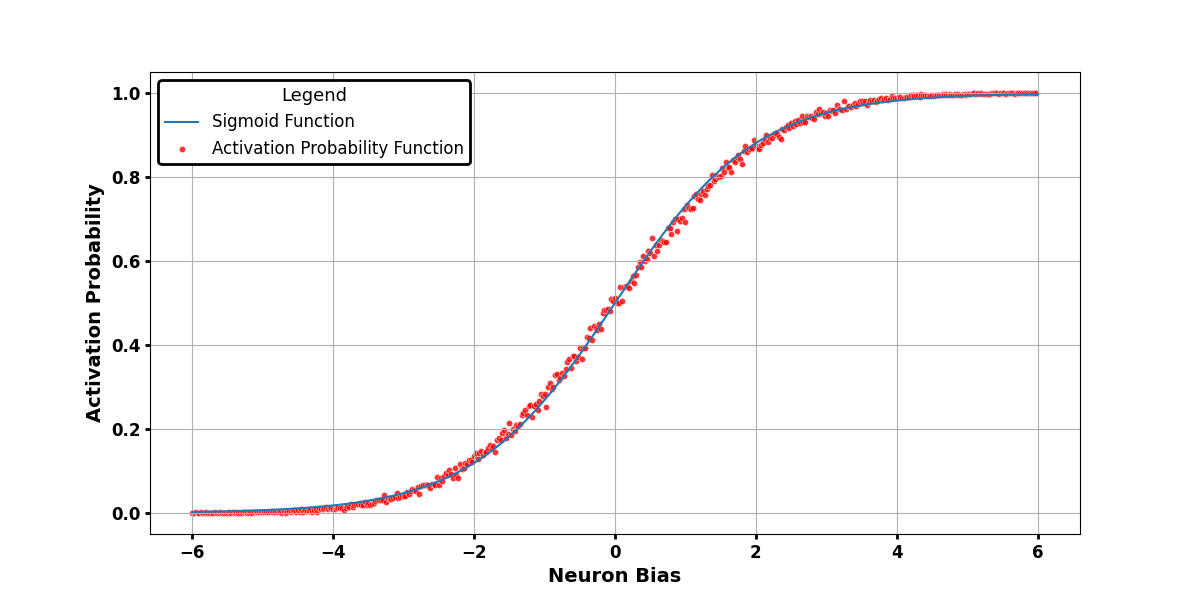
\includegraphics[width=1\linewidth]{graphics/Noisy_HNN_2.png}
    \caption{Noisy activation function of the Hopfield Network imitating the \ac{RBM}}
    \label{Noisy_acitivation_function_good}
\end{figure}
\section{Third Design and Evaluation phase}

Now, that the proof of concept has been validated, this \textbf{Desing Phase} has the goal of connecting the 
Hopfield Network as a sampling method to the \ac{RBM} and therefore enable a complete training. 
This includes using the weights and biases of the \ac{RBM} as an input and performing the sampling with the input.
Finally, the sampled output of the visible and hidden neuron configurations need to be returned, so that the digital computer can update the weights.
With these subgoals the total goal is to enable a complete training of the \ac{RBM} with the sampling method of the Hopfield Network. 
Furthemrore, if the training is successful, the possibility of the N/2 half updating method instead of asynchronously updating of the states should be implemented.
The first technical step is to extend the \texttt{\_rbm.py} to fit the new sampling method: 
\begin{lstlisting}
        if sampling_method == SamplingMethod.GIBBS:
                v_neg = self._sample_visibles(self.h_samples_, rng)
                h_neg = self._mean_hiddens(v_neg)

        elif sampling_method == SamplingMethod.METROPOLIS_HASTING:
            h_neg,v_neg=mcmc_sample(10000,len(self.components_))

        elif sampling_method == SamplingMethod.HOPFIELD_NETWORK:  
            # Hopfield Network Sampling
            v_neg, h_neg = interface_hopfield_sampling(self.components_, self.intercept_visible_, self.intercept_hidden_, iterations_per_theta, N2_HALF=False)    
\end{lstlisting}
Here, the compontents represent the weights of the neurons in the network, while intercept\_visible and intercept\_hidden represent the bias of the neurons. 
Within the, hopfield\_network\_interface\_v2.py, the parameters are taken and an object of the class is initiated. 

\begin{lstlisting}
    def interface_hopfield_sampling(components_, intercept_visible_, intercept_hidden_):
   
        H_net = Hopfield_Net(components_, intercept_visible_, intercept_hidden_)
        H_net.update_network_state()
        
        return H_net.v_neg , H_net.h_neg
\end{lstlisting}
Inside the class, the initialization of all the parameters and weights are performed. 
The update formula needs to calculate the weighted sum, which necessarily requires to know all the weights between the neuron itself, to all the other neurons. 
The decision is to create a weight matrix shown in \ref{attachement:weight_matrix}. 
The function begins by defining the total number of hidden and visible neurons based on the class properties parameters used as input.
These quantities dictate the dimensions of the weight matrix, which, in this instance, results in a matrix of size (100, 64).
This square matrix represents the fully interconnected network, where each neuron can potentially connect to every other neuron, including itself.
As mentioned in 2.2.3, the diagonal elements (self-connections) are set to zero in \ac{RBM}s.

Another important aspect is to maintain the model's symmetry, which is crucial for the energy-based nature of RBMs and the dynamics of Hopfield networks.
Hence, for this reason and simplicity, the weight matrix is initialized as a symmetric matrix using NumPy's np.zeros function.
This ensures that all initial weights are set to zero before being explicitly defined through the components weights.
Scikit Learn randomly initializes the weights by default close to zero, while the biases are set to zero. 
This small weights allow to support an effective gradient distribution which protects against rapid saturation or inefficient learning,
while the bias set to zero allows the network to begin in a neutral position and learn on its own. 

The subsequent nested loops iterates over the indices for hidden and visible neurons to fill the weight matrix.
For each pair of hidden and visible neurons, the corresponding weights are extracted from the components matrix.
This matrix essentially serves as the template for the interactions between hidden and visible layers.
Indexing within the weight matrix is handled carefully, to respect the structure of the RBM. 
Therefore, the decision is to set weights between a hidden neuron i and a visible neuron j at positions \texttt{[i, j+num\_hidden]} and \texttt{[j+num\_hidden, i]} to ensure symmetry.

With some more adjustments necessary to the code the first training of the \ac{RBM} with the sampling method of the Hopfield Network can begin. 
The Hyperparmeters first are set to the same scale(1.75) and same thermalization(100) as for a single neuron but with more sampling steps (5000 sampling steps) than before. 
The results of the traning are visualized in figure\ref{HNN_training}.
\begin{figure}[H]
    \centering
    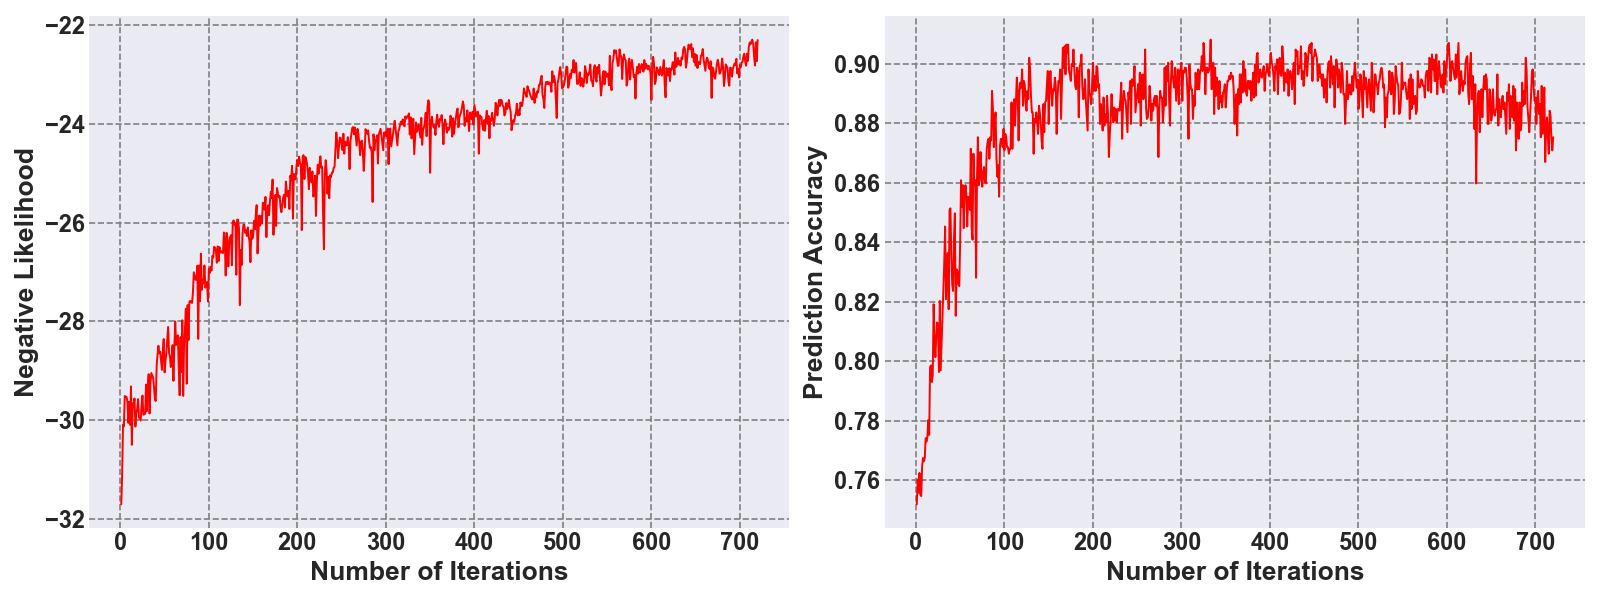
\includegraphics[width=1\linewidth]{graphics/HNN_combined_plot.png}
    \caption{Hopfield Network sampling baselines}
    \label{HNN_training}
\end{figure}
First of all, it can be recognized that the training was successful, which was uncertain. 
Noteworthy, that with this method the output had to be transposed to be able to parse the data Scikit Learn.
In a second look it can be seen that the negative likelihood is far more stable as gibbs sampling and rather has similarities with metropolis hastings sampling.
Here, the best value is a likelihood of -22.3, so slightly worse than metropolis hastings and gibbs sampling. 
The right plot showing the prediction accuracy has the highest ascent of all the three graphs, which proofs that the 
less iterations are required to receive good results compared to the other two methods.
Still, The best prediction value is 90.81\% and therefore worse than gibbs and metropolis hastings. 
The reason for this can be the hyperparameter tuning.
Since the noisy Hopfield Network method can become sensitive fast or is not adjusted correctly 
for this amount of neurons in the network, receiving this result without further adjustments already looks promissing. 

As a result, the following hyperparameters are tuned to possibly received better outcomes. 
Specifically, the scale, which represents the standard deviation and is used as noise is tuned. 
In addition to that the amount of sampling iterations within a single training iteration is tuned.
One extended parameter could be the learning rate and the total iterations but to have an appropriate benchmark against the other two 
sampling methods these parameters are locked in. 
Last but not least, the possibility of tuning the thermalization could help out too even if slightly less significant than the other two hyperparameters.
Since the training takes around 40 minutes to complete tuning too many hypaerparameters takes too much time for the period of this thesis. 
First hyperparameter researched is the influence of the standard deviation (scale) to the maximum prediction accuracy. 
Especially the maximum prediction accuracy of the last 50 training iterations are gathered since this is the relevant area for inference.
Given that the Hopfield Network operates as a statistical sampling method, the standard deviation is also calculated for these final 50 training iterations.
This is done for the scale range of 1.0 to 2.0 within step sizes of 0.05, totalling to 21 single trainings done.
The result is illustrated in figure\ref{Hyperparamers_Scale_ohne}:
\begin{figure}[H]
    \centering
    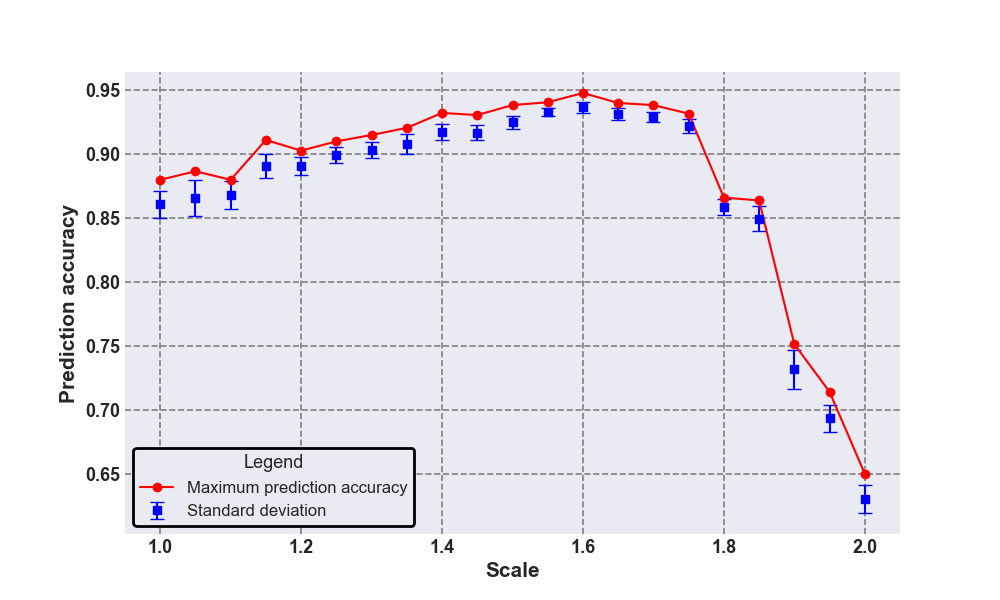
\includegraphics[width=0.9\linewidth]{graphics/NEW_Scale_Ohne_N2_Half_Pred_Acc.png}
    \caption{Hopfield Network Hyperparametertuning scale}
    \label{Hyperparamers_Scale_ohne}
\end{figure}
The result shows that beginning with a scale of 1.0 the prediction accuracy slowly rises until the scale of 1.6
Here, the maximum value is 94.77\% and with that surpasses the performance of both metropolis hastings and gibbs sampling. 
After a scale of 1.75 the prediction accuracy falls off a cliff indicating that the activation function of the \ac{RBM} is not modelled correctly anymore.
This shows that depending an network size and workload the adjustment within this method is important to achieve good results. 
The standard deviation follows the maxmimum prediction accuracy pretty closely and has no outliers indicating that the prediction accuracy is only a lucky random training.
Close to the sclae of 1.0 the deivation is slightly lower compared to the rest of the plot, showing that the scale could be too low to model the sigmoid function correctly. 

In a next step, the best fit with a scale of 1.6 is used for the second hyperparameters. 
The sampling iterations within one training iterations are now tuned.
Hence, the decision is to begin with 1000 sampling iteration continiunig with an increase of 1000 iterations until 15000 iterations are reached. 
With that the training showed that the interesting are is around 1000 to 4000 iteration and that the step size of 1000 is too big for that. 
To be more granular two extra trainings with iterations 1500 ad 2500 werde completed, totalling to 17 trainings performed.
The values are extracted as before, by considering the last 50 iterations and then calculating both the maximum value and the standard deviation from this subset.
The visualized results can be found in following figure\ref{Hyperparamers_Iteraions_ohne}:
\begin{figure}[H]
    \centering
    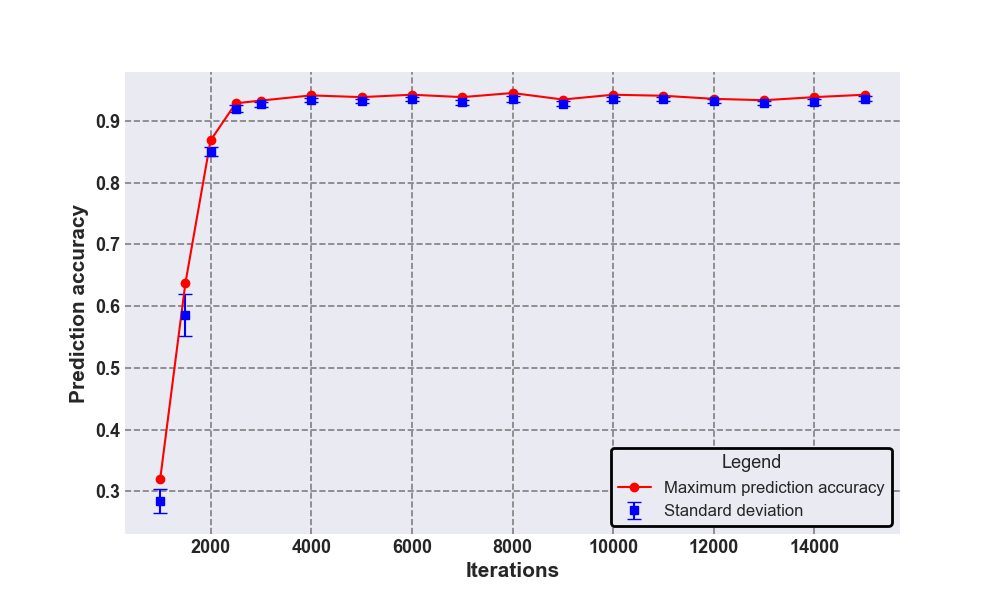
\includegraphics[width=0.9\linewidth]{graphics/Iterations_Ohne_N2_Half_Pred_Acc.png}
    \caption{Hopfield Network Hyperparametertuning sampling iterations}
    \label{Hyperparamers_Iteraions_ohne}
\end{figure}
The line of maximum prediction accuracy starts at the first iteration with a value close to 0.3 and rises rapidly to reach a value just above 0.92 after around 2500 iterations.
From the point of 4000 iterations onwards, the accuracy remains largely constant with slight fluctuations.
The best value is at 15000 iterations with an prediction accuracy of 94.5\%, while at 4000 iterations the accuracy is at 93.35\%.
The error bars indicating the standard deviation are large at the beginning of the graph, which indicates that not enough neurons were updated in the sampling process.
However, with the number of iterations increasing, the error bars become smaller resulting in a more stable accuracy.
Key take away is that after 4000 iterations there are no significant changes to the outcome of the prediction accuracy.

To create a good comparison, the same parameters scale and sampling iterations are tuned for this updating method. 
In this method, 21 complete training sessions are also carried out for this purpose.
Beginning with the scale the result is visualized in figure\ref{Hyperparamers_Scale_mit} :
\begin{figure}[H]
    \centering
    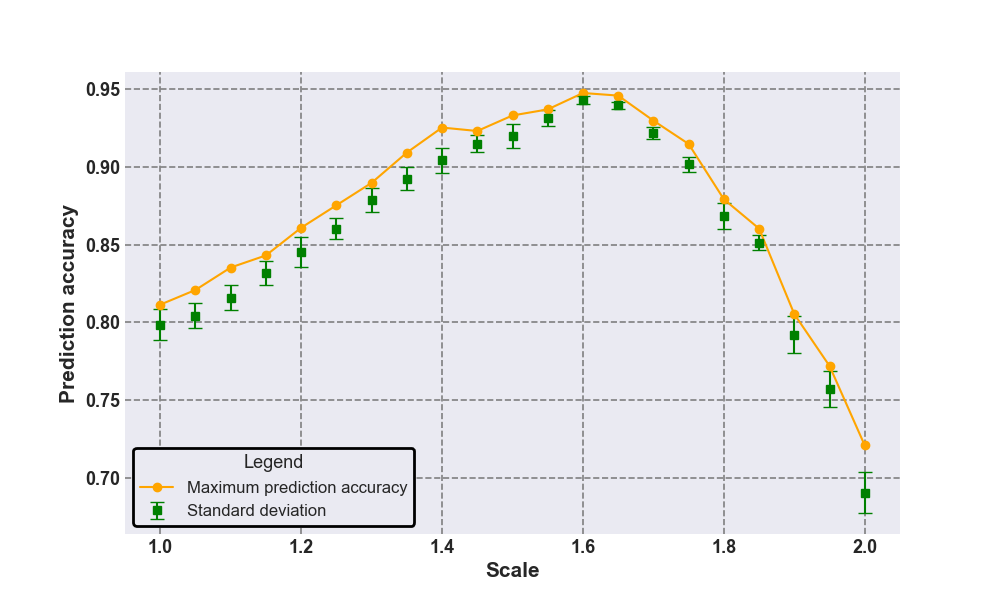
\includegraphics[width=0.9\linewidth]{graphics/NEW_Scale_MIT_N2_Half_Pred_Acc.png}
    \caption{Hopfield Network Hyperparametertuning scale for N/2}
    \label{Hyperparamers_Scale_mit}
\end{figure}
On a first glance, the prediction accuracy beginning from left to right is constantly rising until it reaches the scale of 1.6.
Here, the maximum prediction accuracy tops out at 94.76\%.
What is interesting, that in \ref{Hyperparamers_Scale_ohne} the exact same scale has also the best performance. 
With increasing the scale after the top of 1.6, the accuracy falls off a cliff. 
Noteworthy, is that in comparison with \ref{Hyperparamers_Scale_ohne} the N/2 half updating method has nearly equal prediction accuracy
but is more sensitive. 
This means that the configuration of the hyperparameters is tougher for this updating method and results can get worse more easily. 
The standard deviation represented in the error bars is high at the lower scale values validating that the sigmoid function is not properly mapped. 
This is similar for too high values beginning at a scale of 1.8.

The second hyperparameter are the amount of sampling iterations required to achieve good results. 
In the training process the plan is to begin with the same step sizes like earlier on. Soon it was clear,
that the granularity needs to be much finer too achieve good results. 
Therefore, the decision is to start at iteration 201 (1st iteration after the 200 thermaliation steps) and ending with a sampling iteration of 250 with a step size of 1.
This totals to 50 complete training sessions. The new results are illustrated in figure\ref{Hyperparamers_Iteraions_mit}:
\begin{figure}[H]
    \centering
    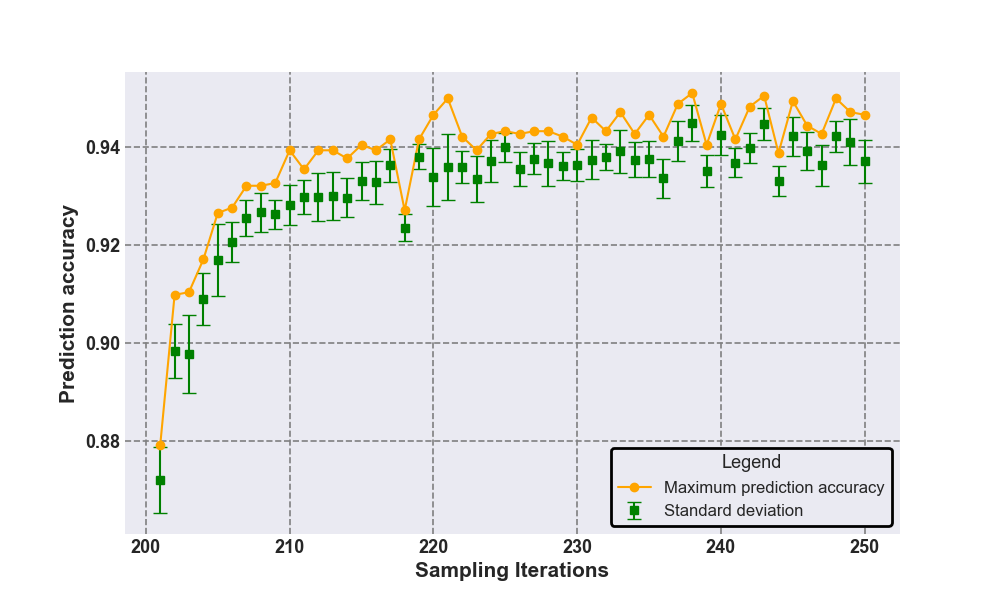
\includegraphics[width=0.9\linewidth]{graphics/Iterations_MIT_N2_Half_Pred_Acc.png}
    \caption{Hopfield Network Hyperparametertuning sampling iterations for N/2 half}
    \label{Hyperparamers_Iteraions_mit}
\end{figure}
The figure shows that with only 10 sampling iterations after the thermalization good prediction accuracies of 94\% can be achieved. 
The maximum prediction value is 95.10\% at 221 sampling iterations, which surpasses the earlier achieved results.
Nonetheless, the key message here is that far less sampling iterations are needed within one big training iteration of the \ac{RBM}
to achieve good results. 
When comparing the number of 221 to the around 4000 sampling iterations required in \ref{Hyperparamers_Iteraions_ohne} it would be more efficient by a factor of 
\(18.09x\). In return, this updating methods saves time and also has less energy consumption required.

With this third design and evaluation phase ending all the functionalities of the prototype are implemented and the prototype itself is complete. 

\section{Final Evaluation phase}
In this final evaluation phase the functional prototype should now be validated within the evaluation phase of the \ac{DSR} framework.
The goal is to answer the research question ``Can Boltzmann Machines be \textbf{efficiently} implemented on physics-inspired
Hardware accelerators by analog noise injection?''.
Since the key word here is efficiently, a simulation will be performed to meassure the parameters required for evaluation.
With the model purpose set, the model scope(time frame) of the simulation introduced in 3.4 is to be considered as short with only mutliple weeks and only one person working on the simulation. 

The next step is to define the result variables. The two variables that are of interest in literature to meassure the performance of the
\ac{mem-HNN} accelerator are troughput (samples/sec) and energy consumption (energy/operation). 
These two metrics are widely used in literature and can create a good comparison.\footnote{cf.\cite{bellettiJanusFPGABasedSystem2009}, p. 54-55; cf.\cite{aaditAcceleratingAdaptiveParallel2023}, p. 1-2; cf.\cite{ortega-zamoranoFPGAHardwareAcceleration2016}, p. 16-17}
Hereby, throughput can be defined as the time needed per Hopfield cycle (sampling iteration) per second.\footcite[cf.][6-7]{bohmNoiseinjectedAnalogIsing2022} 
Meanwhile, the energy consumption is defined by summing over all the single energy consumptions within one sampling iteation.
The resulting unit is called energy/operation. 

Now that the result variables are set the input parameters neeed to be clarified. 
For the throughput knowledge about the autocorrelation of the sampling is required.
Autocorrelation is a statistical measure that captures the degree of correlation between successive configurations generated by timeseries, in this case sampling algorithm for the training of a \ac{RBM}.\footcite[cf.][1-6]{tanakaReductionAutocorrelationHMC2017}
Long correlations between configurations can reduce the effective sample size and lead to inefficiency impacting the precision of the model.
This is important for the result variable ``troughput'' because it allows to know when the sampling is statistically independent and ready to use and therefore how many sampling iterations neeed to be done for an effective training. 
The equation to calculate the statistical dependency of 2 successive samples is the auto-covariance function: 
\begin{equation}
    K_{XX}(t_1, t_2) = \mathbb{E}[(X_{t_1} - \mu_{t_1})(X_{t_2} - \mu_{t_2})] = \mathbb{E}[X_{t_1} X_{t_2}] - \mu_{t_1}\mu_{t_2},
\end{equation}
with \(t_1,t_2\) being two distinct points in time and \(X_{t1},X_{t2}\) are random variables representing the values of the stochastic process at the distinct time points. 
\(\mu_1,\mu_2\) are the mean (expected) values of the random variables \(X_{t1},X_{t2}\). 
The \(\mathbb{E}\) is an expectation operator and is used to calculate the expected value of the expression within the brackets.
Also, the cycle speed of the \ac{mem-HNN} accelerator is needed. 
The clock frequency is around 700MHz and therefore can sample 700 million samples per second, which is about 1.44ns for a single clock cylce.\footcite[cf. table1][7-8]{caiPowerefficientCombinatorialOptimization2020} 
Noteworthy, these numbers are takem from a neural network with 111 neurons. 
On the other hand, the only input variable for the energy consumption is the energy model of the \ac{mem-HNN}, which is introduced in 4.2.1 and is developed by HPE in combination with the Forschungszentrum Jülich.
This allows to meassure each of the individual energy consumptions that are configured to the specifications of the \ac{mem-HNN} hardware accelerator.\footcite[cf.][1-5]{hizzaniMemristorbasedHardwareAlgorithms2023}
For both of the methods one input of course is the finished prototype, that mirrors the functionalities of the \ac{ASIC} on a high level.

With the simulation model specified, the autocorrelation can be implemented into the prototype. 
The decision is to average the values of the output configurations from row to row to an average of 60.
This allows to extract a smoother autocorrelation plot that is not too biased in terms of the statistical approach.
In the attachment\ref{attachement:autocorrelation} the full implementation of the autocorrelation function is available.
To compare the performance of the individual sampling methods in terms of the autocorrelation a threshold is required. 
Here, \(1/\mathrm{e}\) is chosen since it is inspired by many fields, like physics(diffusion length), chemistry and mathematics(half-life as a threshold) etc..\footnote{cf.\cite{archieStatisticalAnalysisHeterozygosity1985}, p. 624-630; cf.\cite{bohmNoiseinjectedAnalogIsing2022}, p. 7-13}
Folliwng results are visualized in following figure\ref{Autocorr comparison}:
\begin{figure}[H]
    \centering
    \includegraphics[width=1\linewidth]{graphics/Visualisierungen_Autocorr_individual_7.png}
    \caption{Autocorrelation for the three sampling methods}
    \label{Autocorr comparison}
\end{figure}

The first row shows the conventional \textbf{Metropolis Hastings} sampling method. On the right plot the autocorrelation
and the according sampling steps are visualized. It can be seen, that the value falls below the threshold at around \textbf{100 sampling steps}, 
Falling below the threshold of \(1/\mathrm{e}\) symbolizes that statistical independent samples are generated.
The left plot therefore meassures the first sampling step within each training iteration that falls below this threshold. 
Here, named correlation time. It can be seen that the the scale on the x-axis in the left plot is higher compared to the other two sampling approaches, 
meaning that metropolis hastings is \textbf{more sensitive}. 

The second row is the \textbf{single neuron Hopfield Network} sampling approach. 
In the right plot it shows that the autocorrelation threshold is reached around after around \textbf{200 sampling steps}.
Even if the value is \textbf{2x worse} than with metropolis Hastings the correlation time for the whole training is \textbf{more stable}.
So even if the initial autocorrelation takes longer over a whole training period the end result has an \textbf{better average} than Metropolis Hastings.

The last approach is the \textbf{N/2 half Hopfield Network}. 
The result verifys the new methods right to exist with only about \textbf{3 iterations} to surpass the threshold in the right plot.
Furthermore, the methods correlation time in the left plot shows that it is by far more \textbf{stable} than the other 2 approaches.
When setting this into perspective even with a conservative average of 5 iterations as correlation time, N2/Half updating therefore
performs \textbf{40x better}, than the single neuron Hopfield Network and \textbf{20x better} than Metropolis Hastings.
When comparing the correlation at the end of the traing iterations, the performance even increases: \textbf{34x better} than the single neuron Hopfield Network (correlation time value of 170) and \textbf{46,6x better} than Metropolis Hastings (correlatin time value of 233).
Surprisingly for this updating method large statistical dependency could be seen in two out of the 720 training iterations.
This means that for these two iterations the autocorrelation \textbf{doesn not fall under the threshold} of \(1/\mathrm{e}\).
The training was attempted three times, and in each instance, the phenomenon occurred between iterations 300 and 500.
Still, this has no impact on the performance of the training and therefore can be seen as outlier.
It is open for further research to identify why this doesn not happen with the other two approeaches and what is the cause.
Since the correct value for not falling under the threshold would be infinity the scale in the plot would be too large. 
Therefore, the same plot with these two outliers can be found in the attachment\ref{attachement:autocorrelation_errors}.

After identifying the autocorrelation of the desired metric, "throughput," it can be calculated by combining the autocorrelation with the cycle speed of the \ac{mem-HNN}.
This is done by taking the autocorrelation time of both Hopfield Network approaches (with N/2 Half and without) and mutlitplying them with the cycle time of the \ac{mem-HNN}.
In addition to that the inverse of the result is calculated resulting in the desired throughput metrics `` samples/second''.
Noteworthy, the cycle time for the \ac{mem-HNN} is 1.44ns for 111 neurons in the network. 
Because the network in this thesis has 164 neurons, the time used for the calculation is estimated to be about 2ns, which can be seen as conservative estimate.
The subsequent visualization\ref{Throughput comparison} shows the throughput for the Hopfield Network:
\begin{figure}[H]
    \centering
    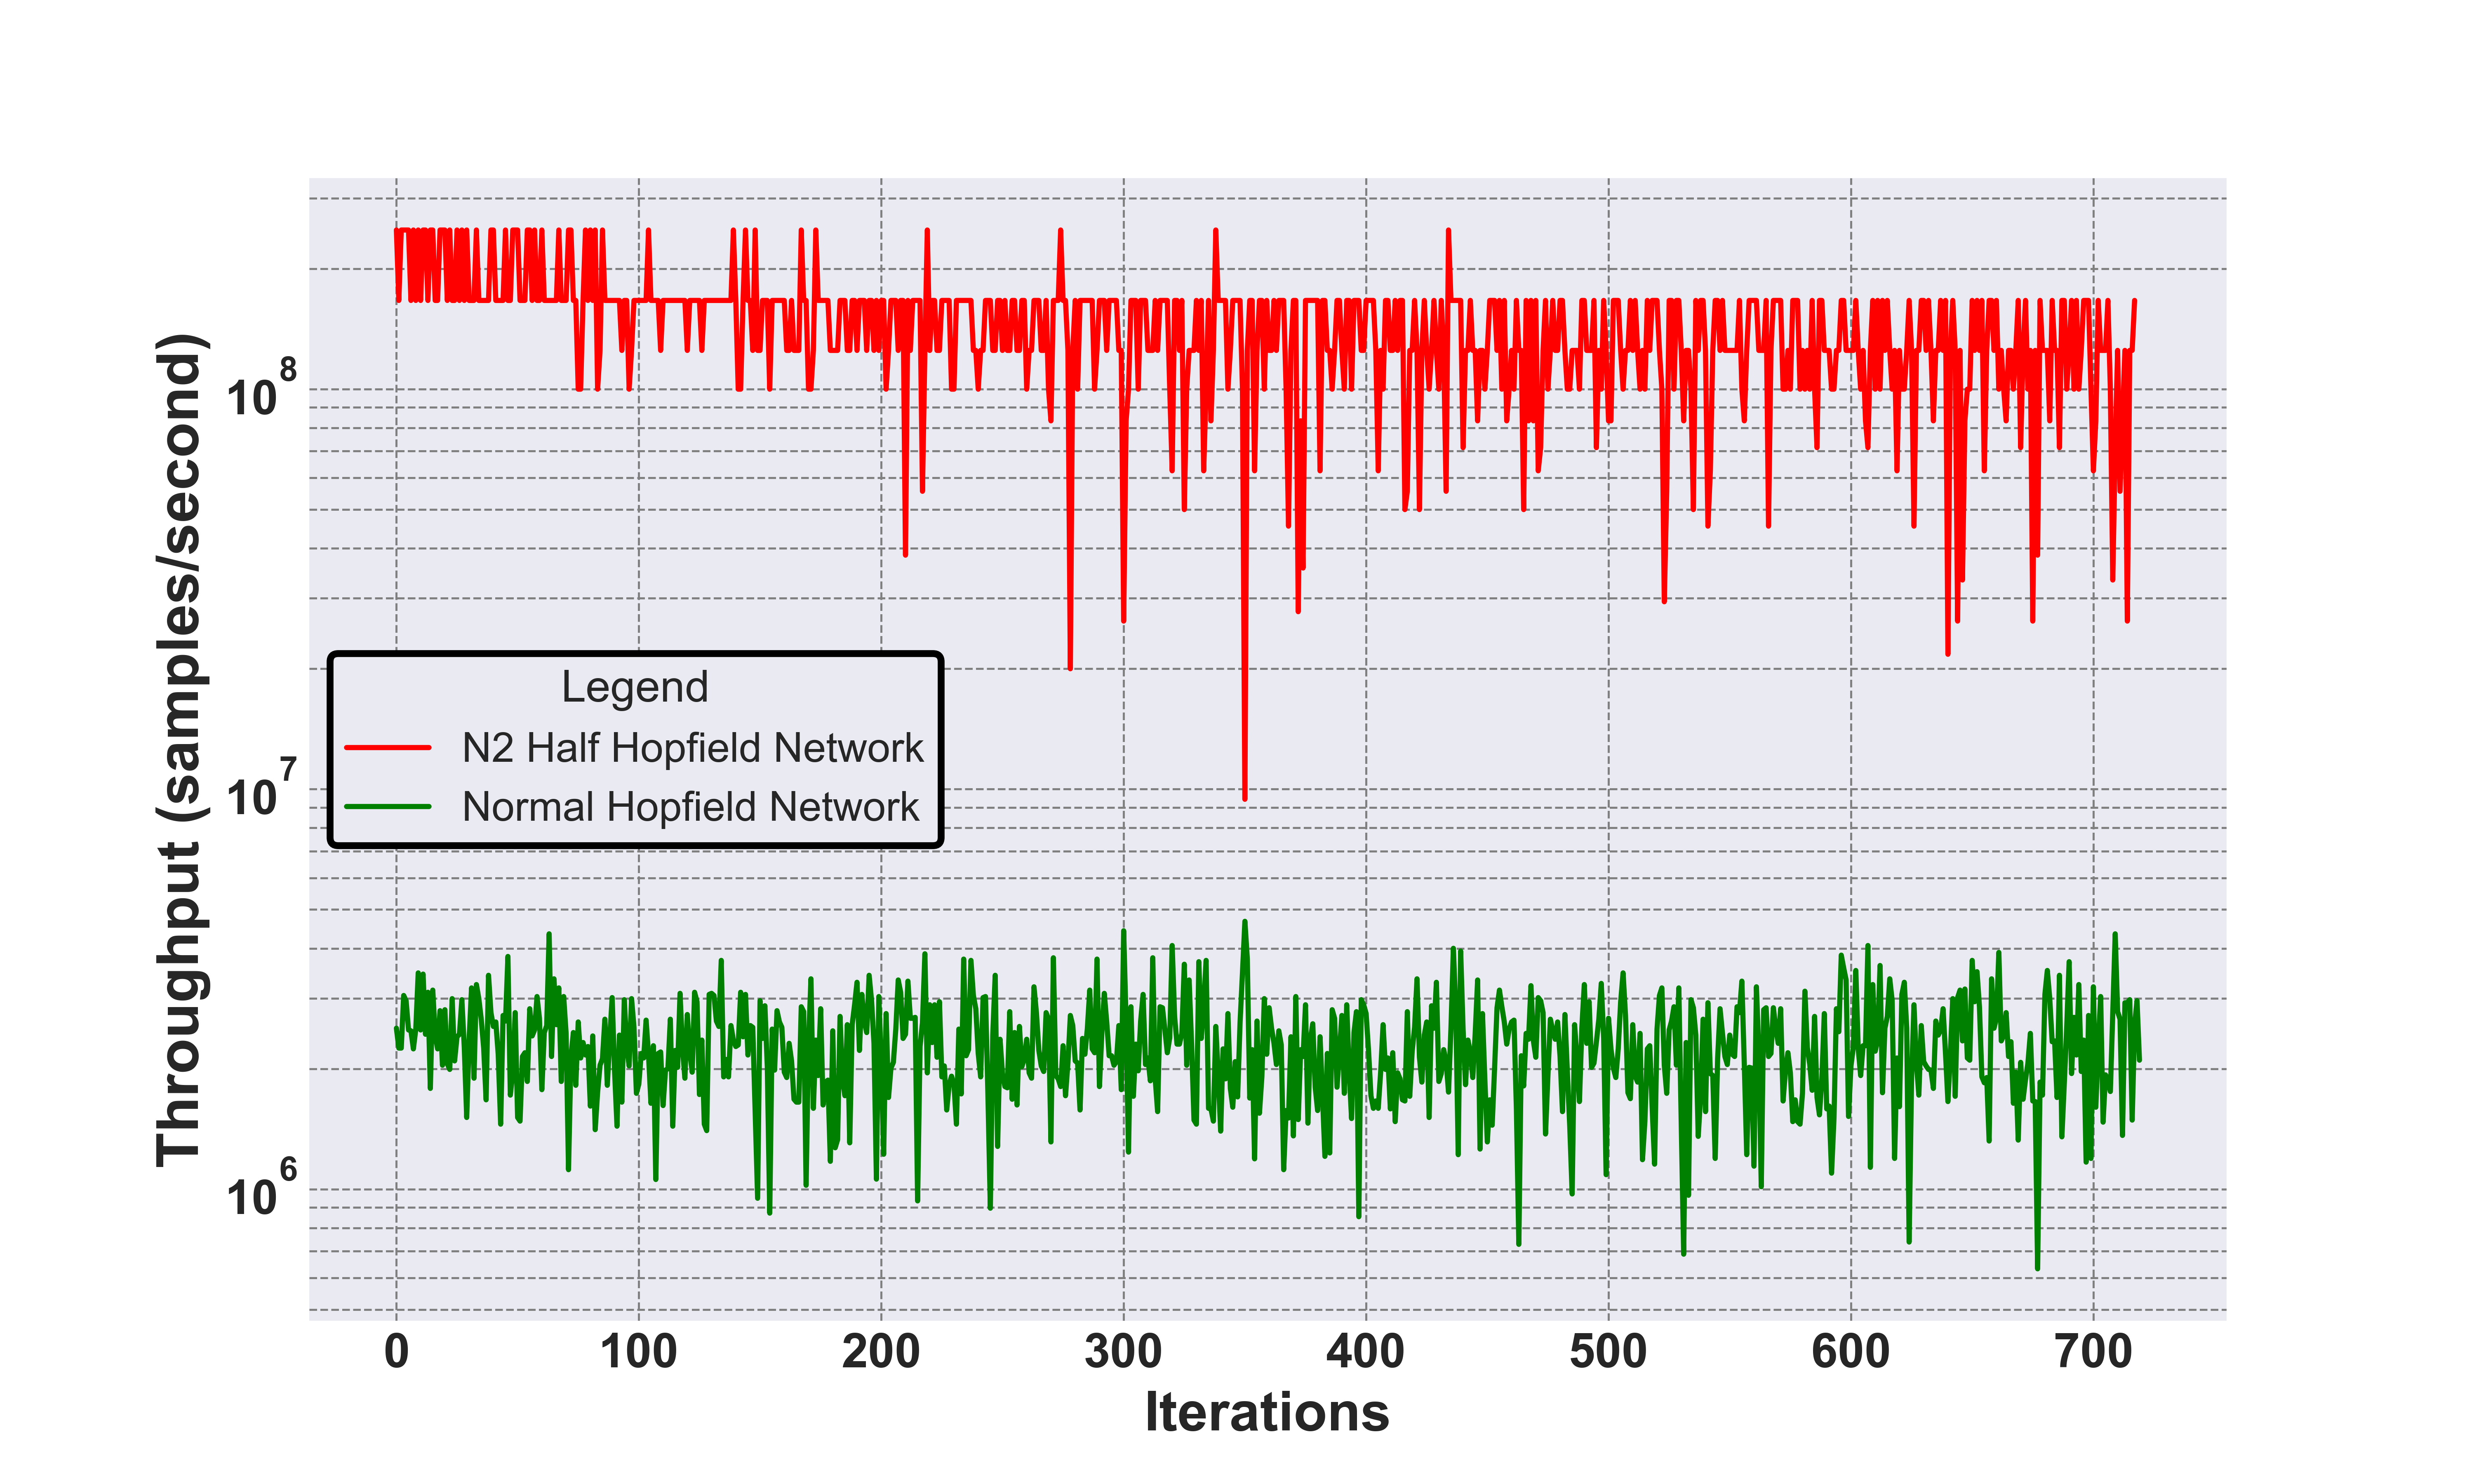
\includegraphics[width=0.8\linewidth]{graphics/Visualisierungen_throughput_log_2.png}
    \caption{throughput}
    \label{Throughput comparison}
\end{figure}
The following results can be gathered when comparing the two lines in terms of efficiency and stability:
The Normal Hopfield Network (green line) displays a stable throughput performance throughout the iterations, consistently above \(\mathbf{10^6}\)
samples per second. This suggests a stable and predictable behavior.
The N2 Half Hopfield Network (red line) exhibits significant variability in throughput. 
While it generally hovers around \(\mathbf{10^8}\) \textbf{to} \(\mathbf{10^9}\) the throughput is more sensitive and fluctuates more compared to the single update approach. 
To get a better feeling of the data, the average of the throughput is calculated: N/2 Half Hopfield Network has
an average of \textbf{144 megasamples/second}, while the
Normal Hopfield Network has an average of: \textbf{2,3 megasamples/second}. 
This means that the computation speed of the N/2 Half method \textbf{is faster} by a factor of \textbf{62.72x}.
Also in the attachment\ref{attachement:throughput_errors} is a version with the outliers included symolizing a throughput of zero for these two iterations.

The results of the autocorrelation implies a low computing time and low energy consumption than with conventional hardware.
To confirm this theory, the second metric to simulate is the \textbf{energy consumption} in energy/operation. 
Hence, the mentioned energy model needs to be implemented into the Hopfield Network interface.
The first adaptation is to \textbf{intialize the energy model} with the size of the neural network (164) as it impacts the size of the crossbar array and influences the overall energy consumption.
An increase in the number of neurons causes a higher energy consumption due to the enlarged crossbar structure.

Afterwards, the two parameters ``a\_pattern'' and ``a\_WL'' need to be calculated.
Hereby, a\_pattern refers to the currents that flow through the respective bitlines.
The current for each bitline is determined by the average of the weighted sum and is accumulated with each iteration.
Subsequently, it is divided by the number of sampling iterations to obtain an average for the respective training iteration.
For an correct calculation and imitation of the \ac{mem-HNN}, there is one more restriction to solve. 
The digital computer generates negative and positive weights and biases, which is not possible in the hardware.
Therefore, the weight matrix needs to be adjusted to handle positive and negastive weights seperately. 
Specifically, the weight matrix is discretized to the according bit resolution of the \ac{mem-HNN}, which is 5bit.
In the ealier design phases, the values were calculated with perfect resolution but for the energy model of the accelerator this is possible. 
Despite the low bit resolution there are many papers that proof that even with a small resolution a good performance can be achieved.\footnote{cf.\cite{maEra1bitLLMs2024}, p. 1; cf.\cite{GitHubHtqinQuantSR}, p. 1; cf.\cite{rouhaniMicroscalingDataFormats2023}, p. 1; cf.\cite{rouhaniSharedMicroexponentsLittle2023}, p. 1}
Since only positive weights can exist within the accelerator, these are separated and written into their own matrix.
This modification is essential to accommodate the hardware constraints that prevent the use of negative weights.

On the other hand, A\_Wl is the average configuration change.
This means This parameter tracks the average changes in configuration within the wordline.
Each time the state changes from 0 (no current) to 1 (current flows), energy is consumed to initially let the metal ions flow.
Therefore, every position in the configuration must be compared with the following configuration position wise.
Subsequently, an average change rate is calculated by dividing by the number of iterations.
This approach quantifies the energy cost associated with state transitions within the network configuration.
An estimate for this, especially for N/2 half is that 25\% of the neurons are updated in one training iteration (50\% randomly drawn and 50\% of that updated).
All the adjustments for the energy model to the interface can be found in the version 5 of the hopfield interface as part of the digital delivery.
The result of the energy consimption is illustrated in following figure\ref{Energy output_2}:
\begin{figure}[H]
    \centering
    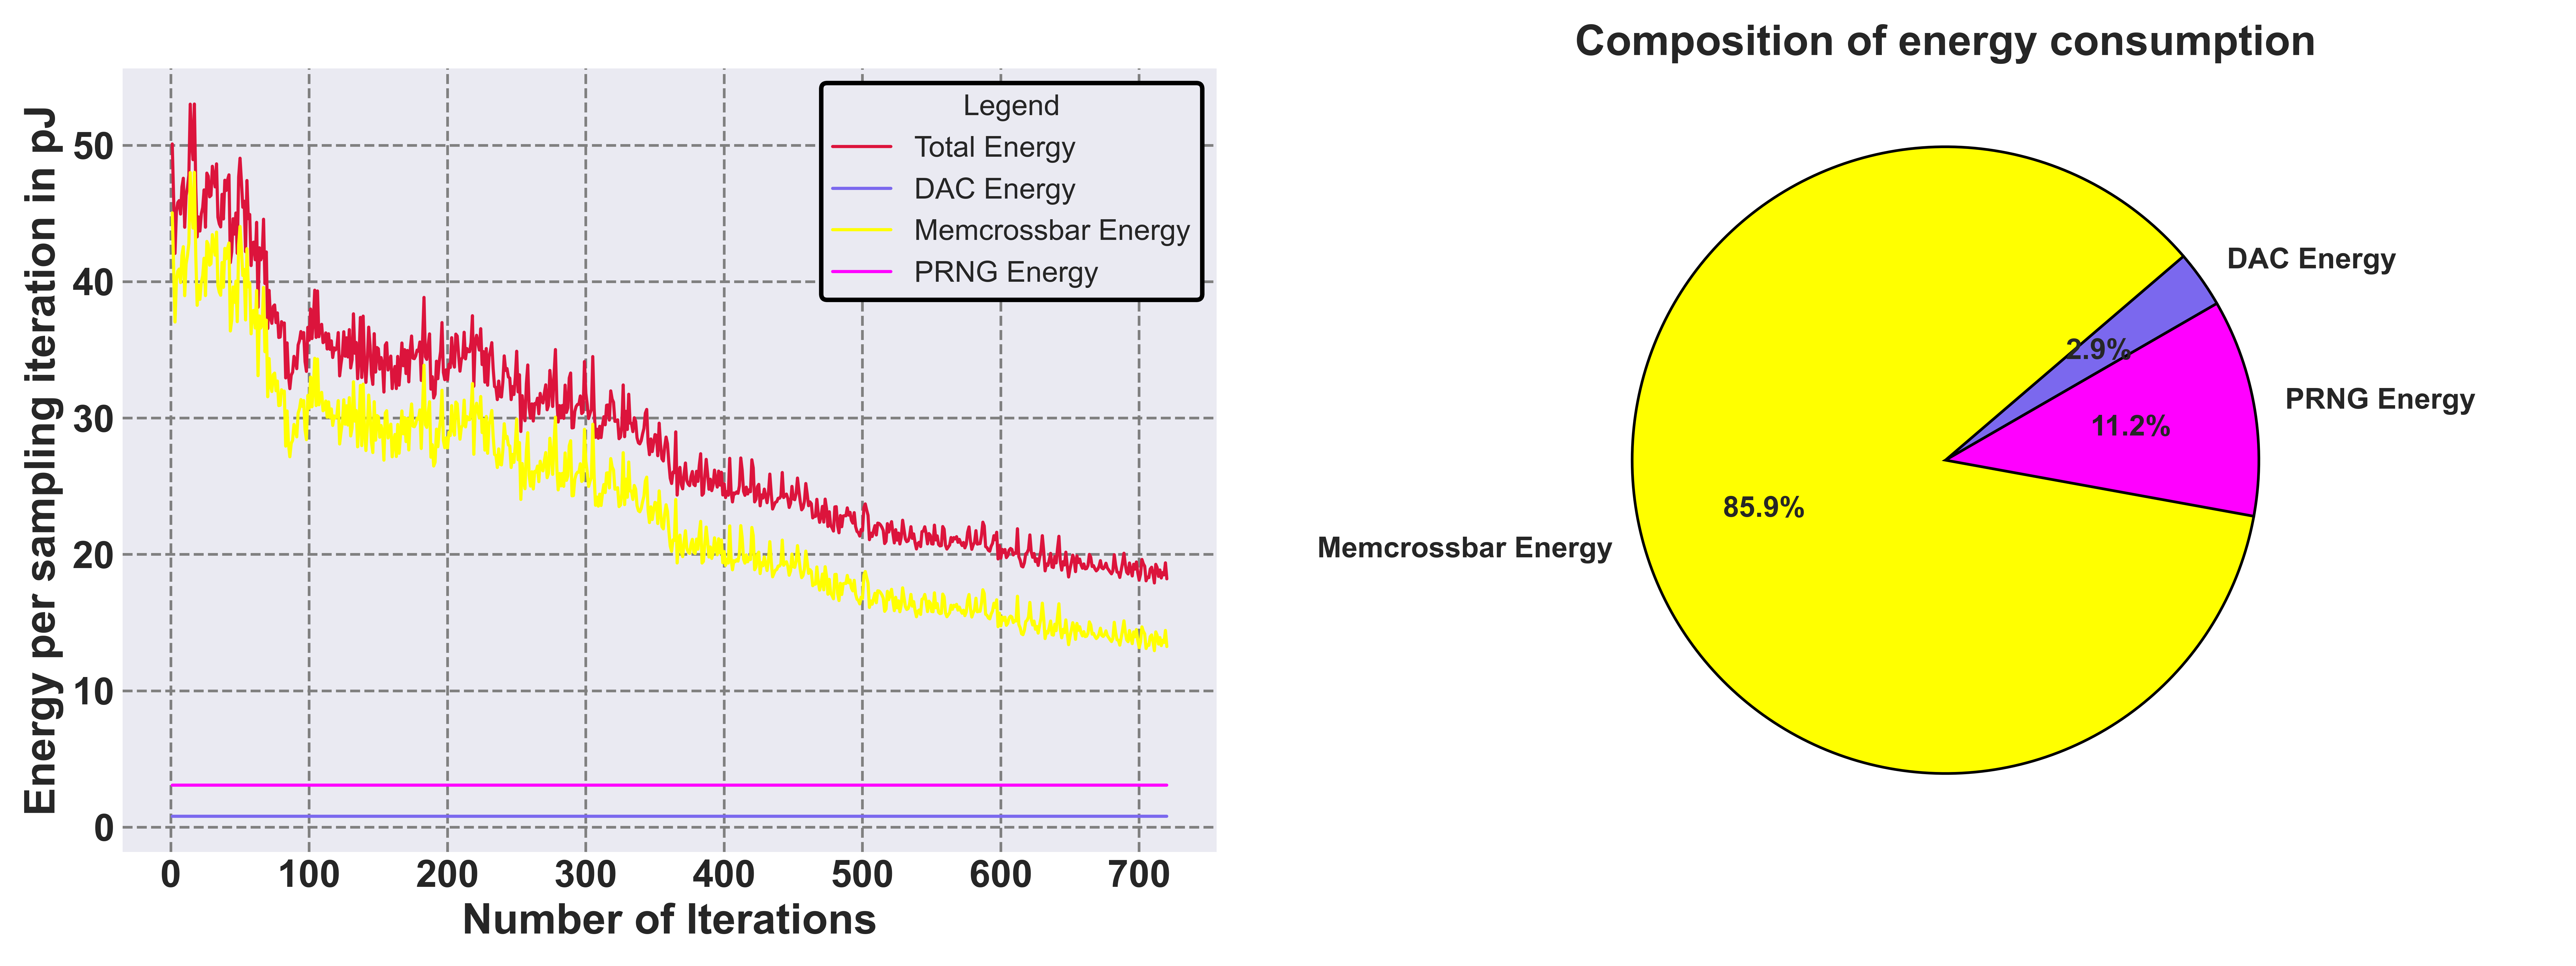
\includegraphics[width=1\linewidth]{graphics/energy_and_averages_plot_4.png}
    \caption{Energy consumption of the \ac{mem-HNN}}
    \label{Energy output_2}
\end{figure}
The left plot shows the energy consumed per sampling iteration (eq.\ to 1 clock cylce of the \ac{mem-HNN}) in piko Joules.
In the beginning of the training the average clock cycle has an total energy consumption of around 45 piko Joules.
Further in the training at atround 100 training iterations the consumption drops to around 35 piko Joules. 
In the end of the training the value falls just below the 20 piko Joules mark. 
The decrease of the energy consumption over the time comes from the weights of the neural netowotk that get better and better configured over time.
Noteworthy, the Memcrossbar energy is the only variable energy consumer that actively changes, while the digital-to-analog converter and the pseudo-random number generator stay horizontal.
A composition of the energy consumption is shown in the right plot.
Here 85\% of the energy is consumed entirely by the Memristor Crossbar and the support entities consume around 15\% of the energy.
The results of the energy model an the energy consumption can be verified by the following paper.\footcite[cf.][4]{hizzaniMemristorbasedHardwareAlgorithms2023}

Finally, it is important to mention that not all hardware components are included. and especially the communication and updating of 
For example the memory and the controller of the \ac{mem-HNN} and are not included in the plot.
Also to consider are the weights in the digital computer, that probably consume 10x the energy of the training on the analog \ac{mem-HNN}. 

In a next step the power consumption of the training is targeted as this delivers a good comparison to other
hardware components like \ac{CPU}s, \ac{GPU}, \ac{ASIC}s or \ac{FPGA}s.
Therefore, the energy per sampling iteration is divided by the time of one clock cycle (2ns) since \(P = \frac{\Delta E}{\Delta t}\).
Furthermore, the right plot is based on the power and cumulates the power multiplied with the sampling iteration to vissualize how much energy the training the neural network consumes for this workload.
\begin{figure}[H]
    \centering
    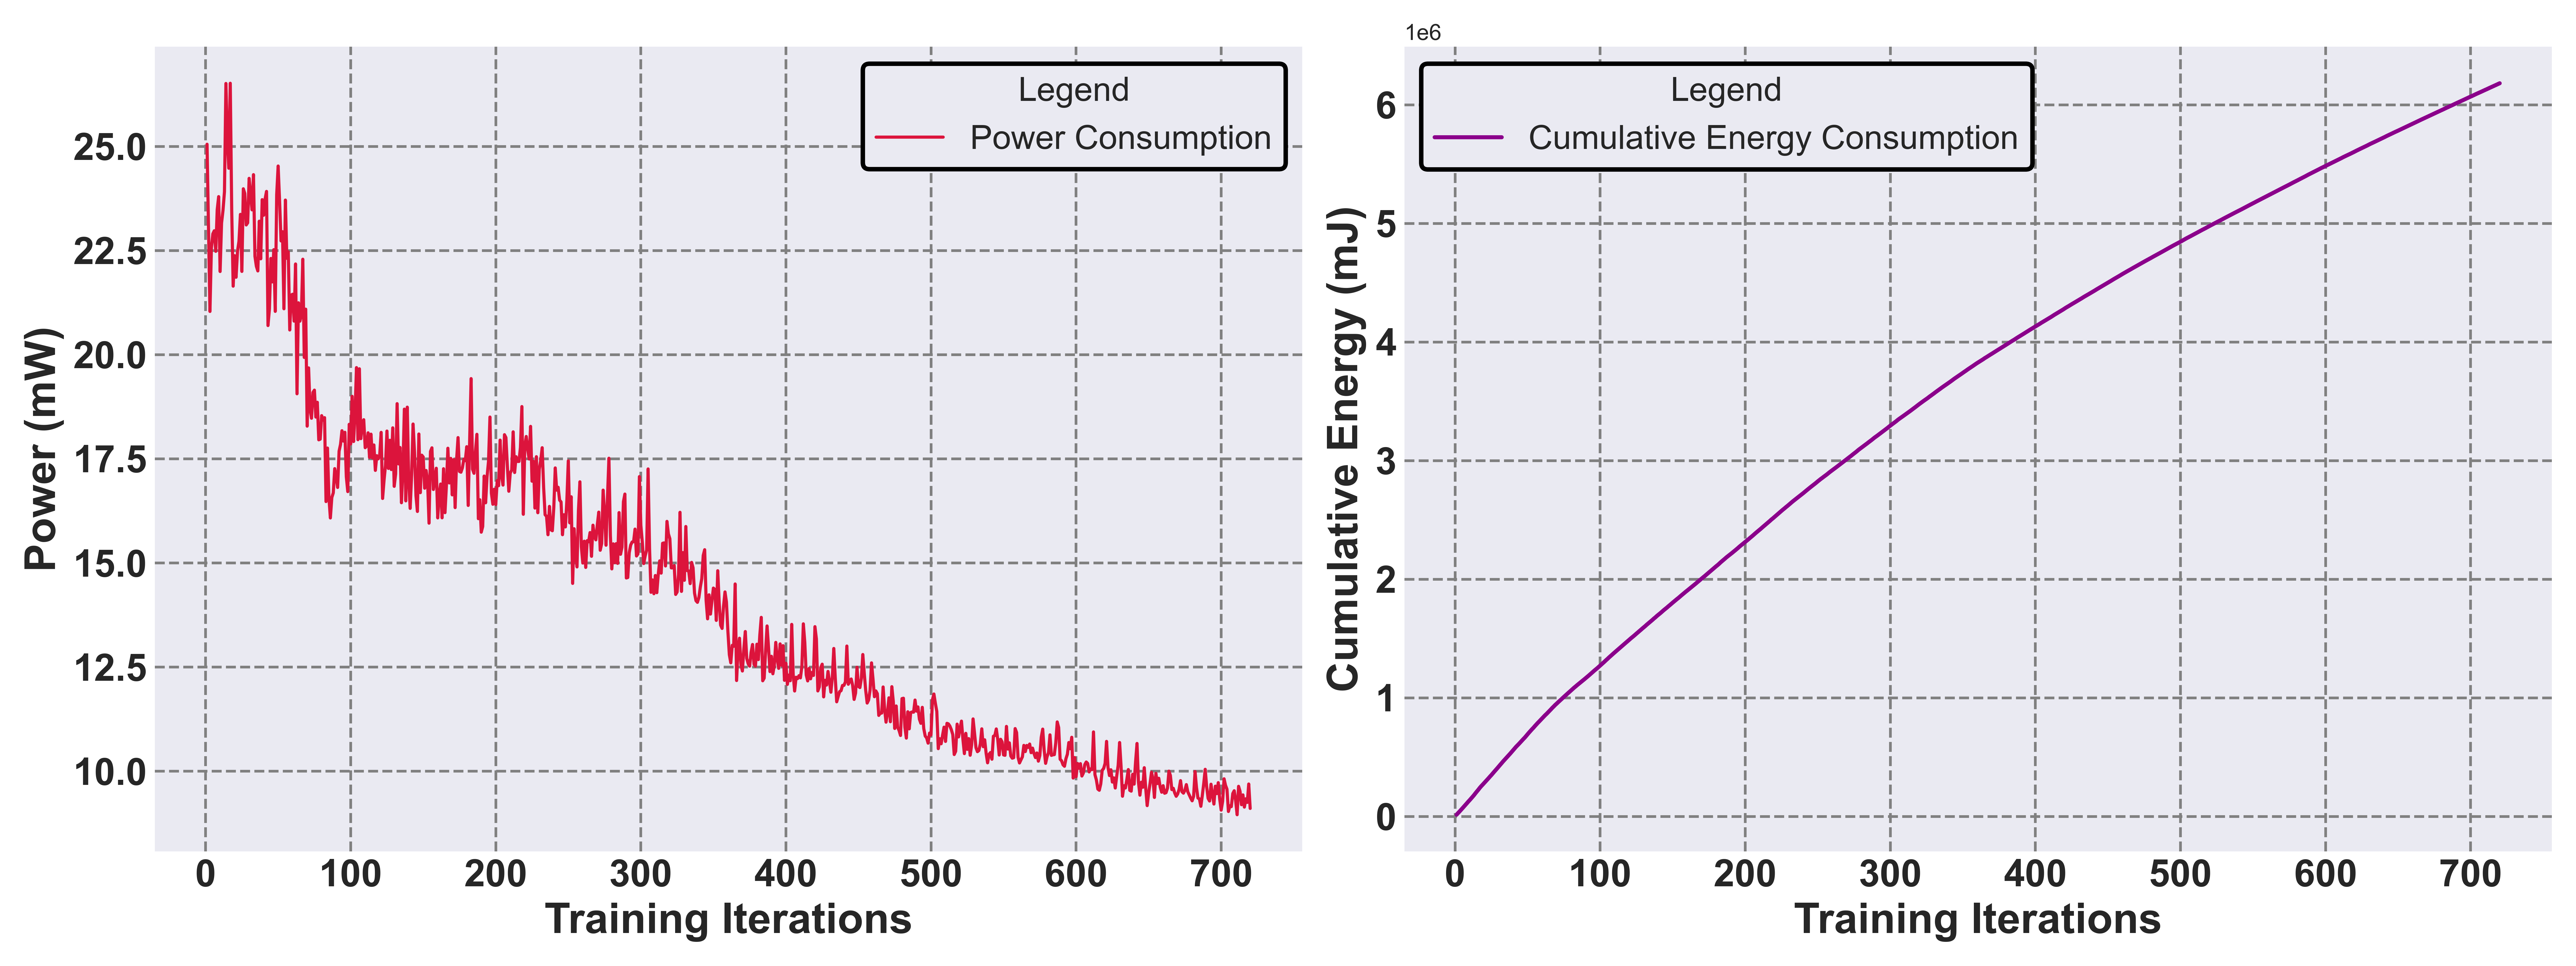
\includegraphics[width=1\linewidth]{graphics/energy_consumption_cumulative_plot.png}
    \caption{Power consumption of the \ac{mem-HNN}}
    \label{Power consumption}
\end{figure}
As shown in figure\ref{Power consumption} the power required to train is around 22.5 mW, which compared to a basic CPU(20-40W)
is significant less. 
Again with training iterations continuing to grow the power consumption decreases. 
At the end of the training around 620 iterations, an power consumption of around 10mW is reached. 
The entire power consumption is mostly stable with some larger fluctuatins in the beginning of the training areound 0 to 70 iterations.
When looking at the right plot, which symbolizes the cumulative energy required for the training in mJ.
Here, it is visible that a complete training with 720 iterations requires around 6.2 mJ. 
Again it is important to keep in mind that these numbers consist of only the \ac{mem-HNN} and do not include the digital computer.                                                                  	                                                                                                                                                                                                                                                                                                                                                                                                                                                                                                                                                                                                                                                                                                                                                                                                                                                                                    

With that the evaluation phase can successfully verify that the models purpose of the simulation, which is to answer the reasearch question, is achieved.
Therefore, Boltzmann Machines can indeed be efficiently implemented on the physics-inspired Hardware accelerator by analog noise injection. 
\chapter{Diffusion and discussion of results}

von Holzweißig: Dieses dient dazu die Ergebnisse des eigenen Beitrags zusammenzufassen
und kritisch zu diskutieren. Auch kann hier der Versuch einer Ergebnisverallgemeinerung
erfolgen.

\section{Zielsetzung und Forschungsmethodik}
\section{Evaluation der Erkenntnisse in Bezug auf die Zielsetzung intrinsisch }
\subsection{Prediction Accuracy}
\subsection{Troughput (Samples/Sec)}
\subsection{Energieverbrauch (Energy/Operation)}
\subsection{Vergleichen mit anderen Hardwarebeschleuniger, FPGA, GPU oder CPU aus der Literatur}
Neue Einsatzmöglichkeit von Hardwarebeschleunigern
für nachhaltigere KI-Modelle: Entwicklung und
Evaluation der Boltzmann Maschinen auf einem
physikinspirierten Hardwarebeschleuniger
\chapter{Kritische Reflexion und Ausblick}
\section{Evaluation der Erkenntnisse in Bezug auf die Zielsetzung der Arbeit }
\section{Kritische Reflexion der Ergebnisse und Methodik}
\section{Ergebnisextration für Theorie und Praxis}
\section{Ausblick}
\chapter*{Appendix}
\addcontentsline{toc}{chapter}{Appendix}
\section*{List of appendices}
\vspace{-8em}

% vor \listofanhang müssen Einrückungen angepasst werden
\abstaendeanhangverzeichnis

\listofanhang
\clearpage
\spezialkopfzeile{Attachment} % damit in der Kopfzeile das Wort "Anhang" angezeigt wird

\lstset{language=TeX, % hervorzuhebende Keywords definieren
  morekeywords={anhang, anhangteil}
}

\definecolor{dkgreen}{rgb}{0,0.6,0}
\definecolor{gray}{rgb}{0.5,0.5,0.5}
\definecolor{mauve}{rgb}{0.58,0,0.82}

\lstset{frame=tb,
  language=Python,
  aboveskip=3mm,
  belowskip=3mm,
  showstringspaces=false,
  columns=flexible,
  basicstyle={\small\ttfamily},
  numbers=none,
  numberstyle=\tiny\color{gray},
  keywordstyle=\color{blue},
  commentstyle=\color{dkgreen},
  stringstyle=\color{mauve},
  breaklines=true,
  breakatwhitespace=true,
  tabsize=3,
  morecomment=[l]{\#} % This line tells 'listings' that '#' introduces a single-line comment
}

\anhang{House of Prototyping Guidelines: Prototyping Dimensions}\label{attachement:prototyping_dimensions}
\begin{figure}[htb]
\centering
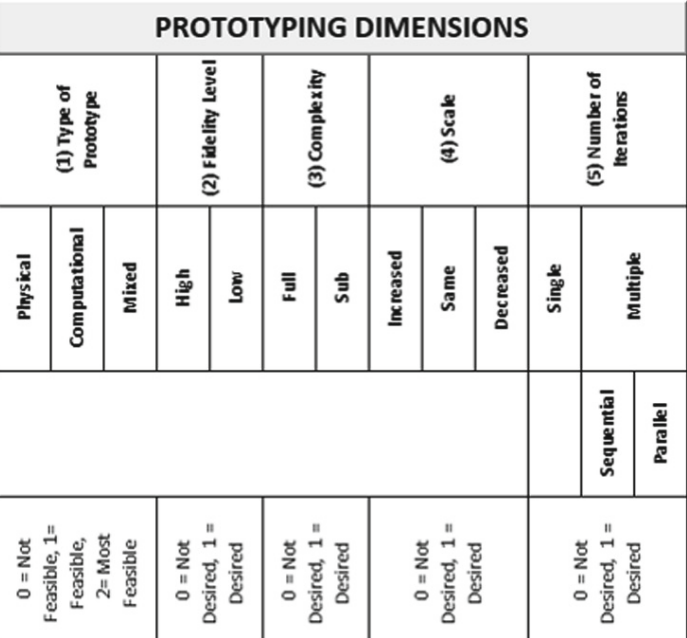
\includegraphics[width=0.9\linewidth]{graphics/Prototyping_dimensions.png}
\caption{Prototyping Dimensions to categorize prototypes}
\end{figure}

\anhang{Weight matrix within the Hopfield Network}\label{attachement:weight_matrix}
\begin{lstlisting}
def initialize_weights_and_biases(self, components):
  num_hidden = self.num_hidden_neurons
  num_visible = self.num_visible_neurons

  #Result size: 100,64

  # Initialize a symmetric weight matrix for simplicity
  self.weights = np.zeros((num_hidden + num_visible, num_hidden + num_visible))

  # Fill in the weights from components for connections between hidden and visible layers
  # for connections between hidden and visible layers
  for i in range(num_hidden):  # Looping through hidden neurons
      for j in range(num_visible):  # Looping through visible neurons
          hidden_index = i
          visible_index = j + num_hidden

          # Additional safeguard: Ensure 'j' is within the bounds of 'components' second dimension
          if j < len(components[0]):
              self.weights[hidden_index, visible_index] = components[i][j]
              self.weights[visible_index, hidden_index] = components[i][j]
          else:
              print(f"Attempted to access components[{i}][{j}], which is out of bounds.")

  return self.weights
\end{lstlisting}

\anhang{Autocorrelation function within the prototype}\label{attachement:autocorrelation}
\begin{lstlisting}
def autocorr(self, x):
        # print("das ist das shape:", x.shape)
        # print("das ist das shape:", x.shape[1])
        average = 60
        leng= 8999-average
        autocorr = np.zeros(leng)
        
        for i in range(0, leng):
            for k in range (0, average):
                autocorr[i] += np.dot(x[:, k]-np.mean(x[:,k]), x[:, k+i]-np.mean(x[:,k+1])) 

        return autocorr / autocorr[0]
\end{lstlisting}

\anhang{Autocorrelation for all sampling methods with outliers}\label{attachement:autocorrelation_errors}
\begin{figure}[H]
  \centering
  \includegraphics[width=0.9\linewidth]{graphics/Visualisierungen_Autocorr_individual_8.png}
  \caption{Autocorrelation for the three sampling methods with outliers}
\end{figure}

\anhang{Throughput with outliers for all sampling methods}\label{attachement:throughput_errors}
\begin{figure}[H]
  \centering
  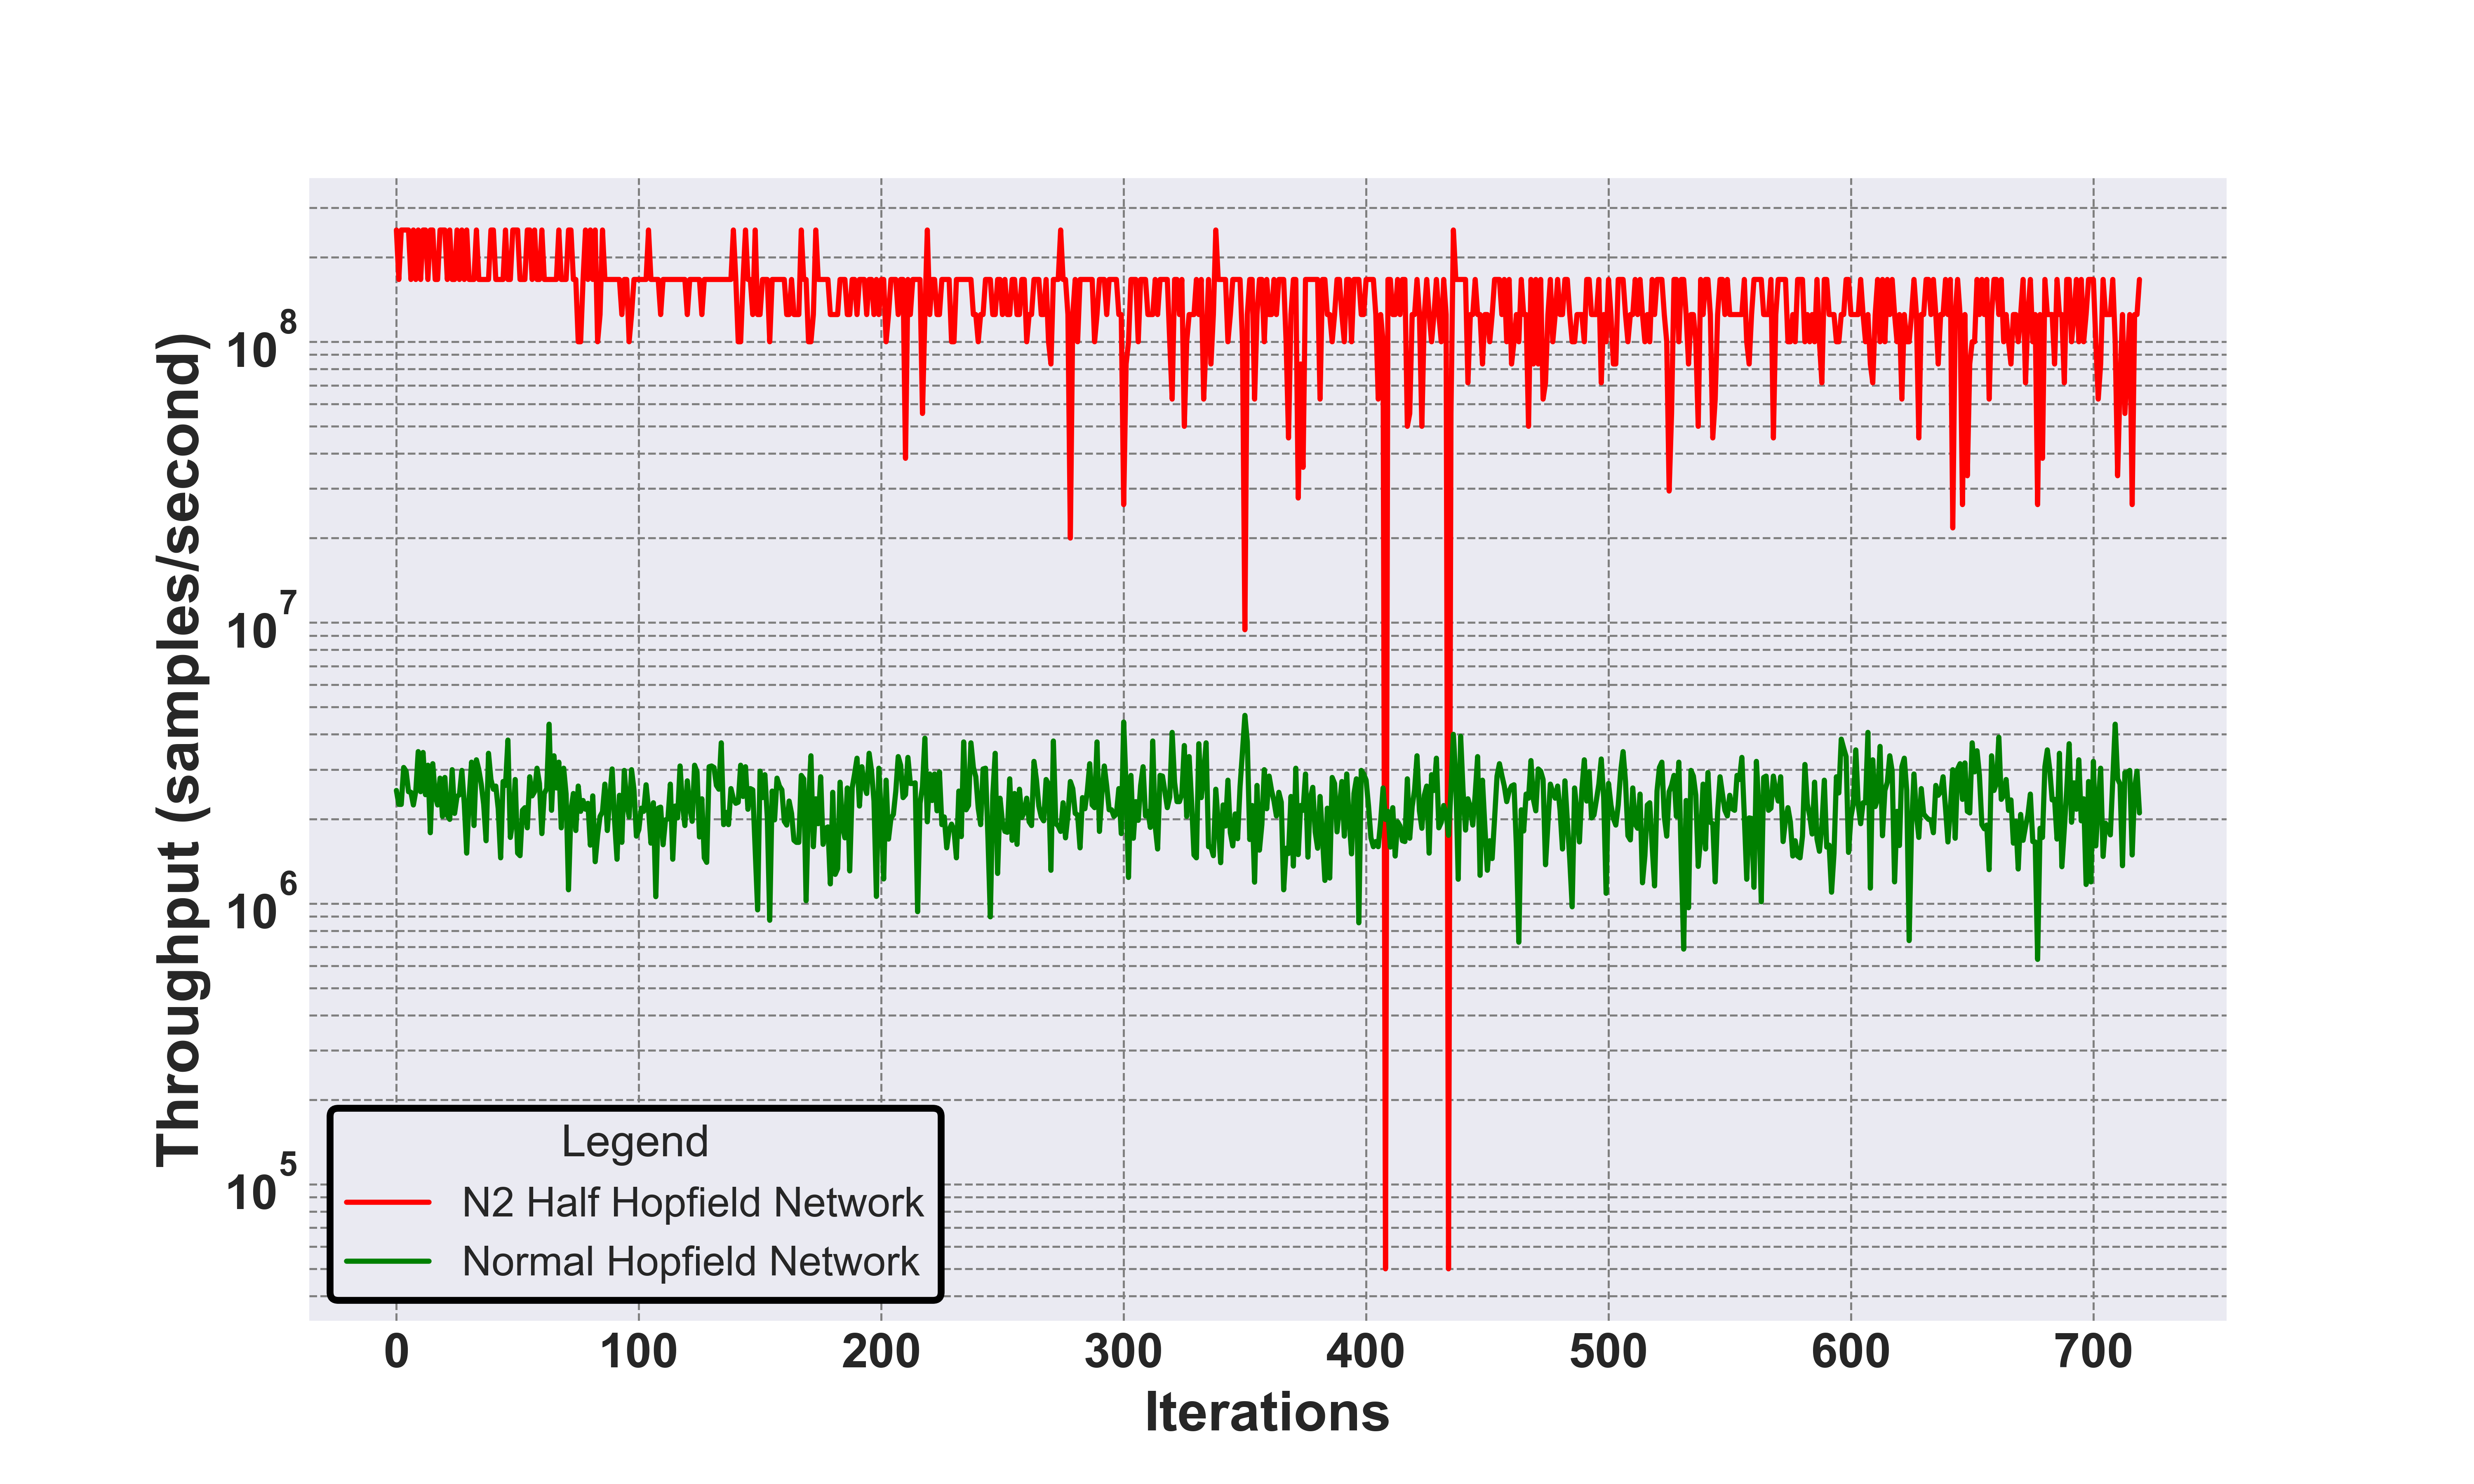
\includegraphics[width=0.8\linewidth]{graphics/Visualisierungen_throughput_log_3.png}
  \caption{Throughput with outliers}
\end{figure}


\anhang{Code for Hopfield Networking upate mechanism with possbility for N/2 Half with outliers for all sampling methods}\label{attachement:HNN_N/2Half Code}
\begin{lstlisting}
  for x in range(self.iterations_per_theta):
              
      if self.N2_Half == False:
          self.neuron_index = np.random.randint(0, self.size) #pick a random neuron in the network
          # Calculate the weighted sum for the neuron, excluding its own state
          weighted_sum = np.dot(self.weights[self.neuron_index, :], self.configuration)               
  
          self.new_configuration = deepcopy(self.configuration)   #copying the old configuration to create a new one and update it
          bias = self.bias[self.neuron_index]
  
          if (weighted_sum + bias + np.random.normal(0, scale=self.scale)) >= self.threshold_theta:           
              self.new_configuration[self.neuron_index] = 1
          else:
              self.new_configuration[self.neuron_index] = 0
  
      else: 
          self.neuron_index = np.random.randint(0, 2, self.size) #pick complete random neurons in the network, result [0,1,1,0] and so on for size of the network
          weighted_sum = np.dot(self.weights[:, :], self.configuration)   
  
          self.new_configuration = deepcopy(self.configuration)
          bias = self.bias 
  
          for i in range(len(self.neuron_index)):
              
              #updating function comparing against threshold
              if self.neuron_index[i] > 0:
                  if (weighted_sum[i] + bias[i] + np.random.normal(0, scale=self.scale)) >= self.threshold_theta:          
                      self.new_configuration[i] = 1
                  else:
                      self.new_configuration[i] = 0
  
      self.configuration = deepcopy(self.new_configuration)   #Saving the new configuration as basic configuration, so for the next iteration it works
  
      if x >= self.thermalization:  
          self.v_neg[:, self.iterationcounter]= self.new_configuration[100:]
          self.h_neg[:, self.iterationcounter]= self.new_configuration[:100]
  
          self.iterationcounter += 1
  
      self.activationProbabilityPerNeuronDict[self.bias] = self.divide_array_elements(self.summedConfigurations, self.iterationcounter)
      self.bias += 0.025
  \end{lstlisting}
%%% Ende des eigentlichen Inhalts %%%


%%% Quellenverzeichnisse (keine Anpassung nötig) %%%
\clearpage
\literaturverzeichnis
%%% Ende Quellenverzeichnisse %%%


%%% Erklärung (keine Anpassungen nötig) %%%
% steht ganz am Ende des Dokuments
\cleardoublepage
\clearpage

\thispagestyle{empty}

{\LARGE\textsf{\textbf{Erklärung}}\bigskip}

% \typMeinerArbeit und \themaMeinerArbeit werden in deckblatt.tex definiert
Ich versichere hiermit, dass ich die vorliegende Arbeit mit dem Thema: \emph{\themaMeinerArbeit} selbstständig verfasst und keine anderen als die angegebenen Quellen und Hilfsmittel benutzt habe.
Ich versichere zudem, dass die eingereichte elektronische Fassung mit der gedruckten Fassung übereinstimmt.

\vspace{3cm}

\begin{center}
\begin{tabular}{ccc}
(Ort, Datum) & \hspace{0.3\linewidth} & (Unterschrift)
\end{tabular}
\end{center}
\end{document}